\documentclass[twoside,11pt]{article}
\usepackage{graphicx,amsmath,latexsym,amssymb}
\usepackage{tikz}
\usepackage{mathdots}
\usepackage[plainpages=false,pdfpagelabels,colorlinks=false,urlcolor=black,pdfpagemode=UseNone,pdfstartview=FitH]{hyperref}
\usepackage{amsthm}
\usepackage{cleveref}
\textwidth 12.5truecm \textheight 19truecm \headsep0.5cm
\oddsidemargin 0.6cm \evensidemargin 1cm \topmargin 1cm


% Heading-------------------------------------------------------------------
\markboth{Your Name }
         {\small{Graph Theory Definitions}}
\date{}

% THEOREM Environments ---------------------------------------------------
\newtheorem{theorem}{Theorem}[section]
\newtheorem{lemma}[theorem]{Lemma}
\newtheorem{proposition}[theorem]{Proposition}
\newtheorem{definition}[theorem]{Definition}
\newtheorem{corollary}[theorem]{Corollary}
\newtheorem{example}[theorem]{Example}
\newtheorem{remark}[theorem]{Remark}
\renewcommand{\theequation}{\thesection.\arabic{equation}}
\renewcommand{\thelemma}{\thesection.\arabic{lemma}}
\renewcommand{\theproposition}{\thesection.\arabic{proposition}}
\renewcommand{\thecorollary}{\thesection.\arabic{corollary}}

\makeatletter
\renewcommand*\env@matrix[1][*\c@MaxMatrixCols c]{%
  \hskip -\arraycolsep
  \let\@ifnextchar\new@ifnextchar
  \array{#1}}
\makeatother


% MATH -------------------------------------------------------------------
\newcommand{\p}{\partial}
\newcommand{\bR}{{\bf R}}
\newcommand{\bC}{{\bf C}}
\newcommand{\bZ}{{\bf Z}}
\newcommand{\bN}{{\bf N}}
\newcommand{\bQ}{{\bf Q}}
\newcommand{\bK}{{\bf K}}
\newcommand{\bI}{{\bf I}}
\newcommand{\bv}{{\bf v}}
\newcommand{\bV}{{\bf V}}
\newcommand{\cF}{{\mathcal F}}
\newcommand{\cA}{{\mathcal A}}
\newcommand{\cB}{{\mathcal B}}
\newcommand{\cC}{{\mathcal C}}
\newcommand{\cL}{{\mathcal L}}
\newcommand{\cX}{{\mathcal X}}
\newcommand{\cY}{{\mathcal Y}}
\newcommand{\cZ}{{\mathcal Z}}
\newcommand{\abs}[1]{\left\vert#1\right\vert}
 \newcommand{\set}[1]{\left\{#1\right\}}
 \newcommand{\seq}[1]{\left<#1\right>}
 \newcommand{\norm}[1]{\left\Vert#1\right\Vert}
 \newcommand{\essnorm}[1]{\norm{#1}_{\ess}}
\newtheorem{thm}{Theorem}[section]
\newtheorem{lem}[thm]{Lemma}
\newtheorem{cor}[thm]{Corollary}
\newtheorem{prop}[thm]{Proposition}
\newtheorem{rem}[thm]{Remark}
\newtheorem{ex}[thm]{Example}
\newtheorem{de}[thm]{Definition}

\def\lf{\left\lfloor}
\def\rf{\right\rfloor}

\newenvironment{pf}
    {{\noindent  \textrm{\textbf{Proof }}}~~}

\numberwithin{equation}{section} \DeclareMathOperator{\Var}{Var}
\DeclareMathOperator{\Ima}{Im}
\DeclareMathOperator{\sgn}{sgn}

\newcommand{\N}{{\mathbb{N}}}
\newcommand{\UU}{\widetilde{U}(F)}
\newcommand{\bpf}{\begin{proof}}
\newcommand{\epf}{\end{proof}}
\newcommand{\bpr}{\begin{proposition}}
\newcommand{\epr}{\end{proposition}}
\newcommand{\bdf}{\begin{definition}}
\newcommand{\edf}{\end{definition}}
\newcommand{\blm}{\begin{lemma}}
\newcommand{\elm}{\end{lemma}}
\newcommand{\bex}{\begin{example}\rm }
\newcommand{\eex}{\end{example}}
\newcommand{\bcor}{\begin{corollary}}
\newcommand{\ecor}{\end{corollary}}
\newcommand{\bthm}{\begin{theorem}}
\newcommand{\ethm}{\end{theorem}}

\newcommand{\be}{\begin{enumerate}}
\newcommand{\ee}{\end{enumerate}}
\newcommand{\bq}{\begin{equation}}
\newcommand{\eq}{\end{equation}}
\newcommand{\bb}{\begin{itemize}}
\newcommand{\eb}{\end{itemize}}
\newcommand{\bpw}{\begin{cases}}
\newcommand{\epw}{\end{cases}}
\newcommand{\B}[1]{\textbf{#1}}
\newcommand{\tn}[1]{\textnormal{#1}}
\newcommand{\bs}{\backslash}
\newcommand{\e}{{\epsilon}}
\newcommand{\gs}{{\sigma}}
\newcommand{\ve}{{\varepsilon}}
\newcommand{\bfrac}[2]{\displaystyle \frac{#1}{#2}}
\newcommand{\ds}[1]{\displaystyle {#1}}
\newcommand{\dsum}[2]{\ds{\sum_{#1}^{#2}} }
\newcommand{\ora}[1]{\overrightarrow{#1}}
\newcommand{\ra}{\rightarrow}
\newcommand{\Z}{{\mathbb Z}}

% -------------------------------------------------------------------
\begin{document}
\hypersetup{pageanchor=false}
\thispagestyle{empty}
% ---------------------TITLE----------------------------------

\centerline {\bf Graph Theory Project}

\vskip.2cm

\centerline{ \today}

\section{Definitions}

\bdf
{\bf (Graph)}
A {\it graph}, $G$, consists of a vertex set $V(G)=\{v_1, v_2, \dots, v_n\}$ and an edge set $E(G)\subseteq \{\{x, y\}\textrm{ or } (x,y) |\ x, y \in V(G)\ \text{where}\ x \neq y \}$.
\edf

\bdf
{\bf (Digraph)}
A {\it directed-graph} or {\it digraph} is a pair $(V,E)$, where $V$ is a nonempty set of vertices, and $E$ is a set of directed edges between the vertices. To complete this definition, we define a {\it directed edge} to be an object which has two properties associated with it: a starting node, and an ending node.
\edf

\bdf
{\bf (Order of a Graph)}
The order of a graph of $G$ the number of vertices in G, $|V(G)|=n$.
\edf

\bdf
{\bf (Adjacency Matrix)}
Let $G$ be a graph. The {\it adjacency matrix} of the graph is the
$n \times n$ matrix $A(G) = [a_{ij}]_{n \times n}$
such that
\begin{displaymath}
a_{ij} =  \left\{\begin{array}{ll} 1 & \textrm{if $ \{v_i, v_j\} \textrm{ or } (v_i,v_j) \in E(G)$ }
 \\ 0 & \textrm{otherwise }
\end{array}\right.
\end{displaymath}
We denote {\it the determinant of a graph} $G$ as $det(A(G))=|G|$.
\edf

\bdf
{\bf (Degree of Vertex)}
Let $G=(V,E)$ be a graph. the {\it degree of a vertex} $v\in V(G)$ is the number of edges attached to $v$, denoted as $deg(v)$.
\edf

\bdf
{\bf (Indegree of Vertex)}
Let $G=(V,E)$ be a directed graph. the {\it indegree of a vertex} $v\in V(G)$ is the number of  directed edges going into $v$, denoted as $indeg(v)$.
\edf

\bdf
{\bf (Outdegree of Vertex)}
Let $G=(V,E)$ be a directed graph. the {\it outdegree of a vertex} $v\in V(G)$ is the number of directed edges going out of $v$, denoted as $outdeg(v)$.
\edf

\bdf
{\bf (Degree Matrix)}
Let $G=(V,E)$ be a graph with $|V|=n$. The {\it degree matrix} is a $n\times n$ diagonal matrix $D(G) = [d_{ij}]_{n \times n}$ such that
\begin{displaymath}
d_{ij} :=  \left\{\begin{array}{ll} deg(v_i) & \textrm{if $i=j$ }
 \\ 0 & \textrm{otherwise }
\end{array}\right.
\end{displaymath}
\edf

\bdf
{\bf (Indegree Matrix)}
Let $G=(V,E)$ be a directed graph with $|V|=n$. The {\it degree matrix} is a $n\times n$ diagonal matrix $ID(G) = [d_{ij}]_{n \times n}$ such that
\begin{displaymath}
d_{ij} :=  \left\{\begin{array}{ll} indeg(v_i) & \textrm{if $i=j$ }
 \\ 0 & \textrm{otherwise }
\end{array}\right.
\end{displaymath}
\edf

\bdf
{\bf (Outdegree Matrix)}
Let $G=(V,E)$ be a directed graph with $|V|=n$. The {\it outdegree matrix} is a $n\times n$ diagonal matrix $OD(G) = [d_{ij}]_{n \times n}$ such that
\begin{displaymath}
d_{ij} :=  \left\{\begin{array}{ll} outdeg(v_i) & \textrm{if $i=j$ }
 \\ 0 & \textrm{otherwise }
\end{array}\right.
\end{displaymath}
\edf

\bdf
{\bf (Laplacian Matrix)}
Let $G=(V,E)$ be a graph with $|V|=n$. The {\it Laplacian matrix} is a $n\times n$ diagonal matrix $L(G)$ defined as
$$ L(G)=D(G)-A(G)  $$
\edf


\bdf
{\bf (In-Laplacian Matrix)}
Let $G=(V,E)$ be a graph with $|V|=n$. The {\it in-Laplacian matrix} is a $n\times n$ diagonal matrix $IL(G)$ defined as
$$ IL(G)=ID(G)-A(G)  $$
\edf

\bdf
{\bf (Minor)}
Let $A$ be $n\times n$ matrix. The minor of $A$ is a $(n-1)\times (n-1)$ matrix obtained by removing the $i$th row and $j$th column from $A$. We denote the minor of $A$ at the $A_{ij}$ entry as $Minor(A_{ij})$.
\edf

%\bdf {\bf{(Directed Handle Graph)}}
%For a graph $G$ of order $m$ and vertices $u,v\in V(G)$, we denote $G_{(u,v)}$ to be the graph where a directed edge from vertex $u$ to vertex $v$ is added to $E(G)$. We refer to this as the directed graph handle $(u,v)$. further more we refer to the starting node $u$ as the outflow point, and $v$ is referred to as the inflow point with $u$ and $v$ being handle pairs. In the case that multiple handles are added $G_{(u_{1},v_{1}),(u_{...},v_{...}),(u_{n},u_{n})}$ will represent the handles of the graph being added. This will also be referred to as $H(G)$.
%\edf

\bdf {\bf{(Directed Vertex Handle Graph)}}
For a graph $G$ of order $m$ and vertices $u,v\in V(G)$, we denote $VH(G)_{(u,v)}$ to be the graph where a new vertex $w$ is added to $V(G)$ and a directed edge from vertex $u$ to vertex $w$ which will be referred to as the outflow edge and a directed edge from vertex $w$ to vertex $v$  which will be referred to as the inflow edge are added to $E(G)$. Vertex $w$ is called \rm the directed graph handle vertex \it of the directed graph handle $(u,v)$. Furthermore we refer to the starting node $u$ as the outflow point, and $v$ is referred to as the inflow point, while $w$ is referred to as the reservoir point. This will also be referred to as $VH(G)$
\edf


\bdf
{\bf (Path Graph)}
A {\it path graph } ${P_m},$ $m\geq 1$ is a undirected graph with $m$ vertices,
vertex set $V({P_m})=\{1,2,...,m\}$ and an edge set $E({P_m})=\{\{1,2\},\{2,3\},...,\{m-1,m\}\}.$
\edf

\bdf
{\bf (Cycle Graph)}
A {\it cycle graph } ${C_m},$ $m\geq 3$ is a undirected graph with $m$ vertices, vertex set  $V({C_m})=\{1,2,...,m\}$ and an edge set $E({C_m})=\{\{1,2\},\{2,3\},...,\{m-1,m\}, \{m,1\}\}.$
\edf

\bdf
{\bf (Directed Path)}
A {\it directed path } $\ora{P}_m,$ $m\geq 1$ is a digraph with $m$ vertices, a vertex set
 $V(\ora{P}_m)=\{1,2,...,m\}$ and an edge set $E(\ora{P}_m)=\{(1,2),(2,3),...,(m-1,m)\}.$
$$\overset{1}{\bullet}\ra \overset{2}{\bullet} \ra \cdots \ra \overset{m}{\bullet}$$
\edf

\bdf
{\bf (Directed Cycle)}
A {\it directed cycle } $\ora{C}_m,$ $m\geq 2$ is a digraph with $m$ vertices, a vertex set
$V(\ora{C}_m)=\{1,2,...,m\}$ and an edge set $E(\ora{C}_m)=\{(1,2),(2,3),...,(m-1,m),(m,1)\}.$
\edf

\bdf
{\bf (SubGraph)}
Let $G= (V,E)$ be a digraph.  We say $H= (V,F)$ is a subgraph of $G$ if $F \subset E$.  Note that $G$ and $H$ share the same vertex set.
\edf

\bdf
{\bf (Spanning Subgraph)}
A {\it spanning subgraph} $S$ of a digraph (or graph) $G$ is a subgraph such that $V(S)=V(G)$.
\edf

\bdf
{\bf (Path)}
Let $G$ be a digraph and let $x$, $y \in V$.  A path from $x$ to $y$ is a sequence of alternating vertices and edges \({x = x_1,e_1,x_2,...,x_{k−1},e_{k−1},x_{k} = y}\) where $e_i$ is an edge from $x_i$ to $x_{i+1}$ for all $1 \leq i < k$ and where all the vertices and edges are unique.
\edf

\bdf
{\bf (Connected)}
Let $G$ be a digraph, and let $x$,$y \in V$.  Then $x$ is said to be connected to $y$ if there exists a path from $x$ to $y$.
\edf

\bdf
{\bf (Tree)}
A tree is a connected graph with no cycles.
\edf

\bdf
{\bf (Directed  Rooted Tree)}
Let $G=(V,E)$ be a graph with $|V|=n$ and $v_i \in V(G)$, where $i$ is an integer with $1\leq i \leq n$.
We say $G$ is a directed  rooted tree rooted at $v_i$, or spanning tree, if there is a unique path from $v_i$ to $v_j$ for all $j=1,...,i-1,i+1,...n$.
\edf

\bdf
{\bf (Spanning Tree)}
Let $G=(V,E)$ be a graph. A tree $T$ in $G$ is a spanning tree if $V(T)= V(G)$. 
\edf

\bdf
{\bf (Rooted Node)}
The rooted node is the vertex $v \in V(G)$ such that $T(G)$ is generated by $v$.
\edf

\bthm
{\bf Matrix-Tree Theorem for Digraphs} 
Let $G = (V,E)$ be a spanning tree digraph rooted at $v\in V(G)$. Then the number of directed rooted tree at $v$ is equal to the determinant of the minor of the Laplacian matrix of G, $Minor(L(G)_{ij})$, for the $ij$th entry is where the root $v$ is. 
\ethm

\section{One Handle.}
\blm
\label{symhandle}
Let $VH_n(G)$ be a directed vertex handle graph of $G$ with $n$ handles. Let $r$ be the outflow vertex of one of the handles, and let $v$ be the inflow vertex of the same handle.
Let $T$ be a spanning tree in $VH_n(G)$ such that $T$ is rooted at $r$. Then there does not exist a path $p\in G$ from $r$ to $v$. 
\elm

\bpf
Let $VH_n(G)$ be a directed vertex handle graph of $G$ with $n$ handles. Let $r$ be the outflow vertex of one of the handles, and let $v$ be the inflow vertex paired with $r$.
Let $T$ be a spanning tree in $VH_n(G)$ such that $T$ is rooted at $r$.  Suppose there exists a path $p\in G$ from $r$ to $v$. By definition of spanning tree, there exists a directed path $p'$ from the root $r$ using the inflow edge and outflow edge to $v$. But this contradicts with our assumption that $T$ is a spanning tree because the path $p$ and $p'$ will create a cycle in $T$. Therefore, there does not exists a path in $G$ from the outflow vertex to the inflow vertex.
\epf

\bdf
Let $G$ be a graph. Denote $\tau(G)$ as the number of trees in $G$, and denote $T (G)$ as the set of all spanning tree in $G$,\\ $T(G):=\{g\in G \; |\;g \text{ is a spanning tree}  \}$.
\edf

\bdf
\label{crd_bij}
Let $A,B$ be finite sets. $A$ has the same cardinality as $B$, denoted $|A|=|B|$, if and only if there is a bijection from $A$ to $B$.
\edf

\blm
\label{bij_count}
Let $G=(V,E)$ be a graph, and let $v'$ be a vertex such that $v'\notin V(G)$. Let a graph $G':= (V(G)\cup \{v'\}, E(G)\cup \{e\})$, with  $e$ being a directed edge from some vertex $v\in V(G)$ to $v'$. Then $\tau(G)=\tau(G')$.
\elm
\bpf
Let $G=(V,E)$ be a graph, and let $v'$ be a vertex such that $v'\notin V(G)$. Let a graph $G':= (V(G)\cup \{v'\}, E(G)\cup \{e\})$, with  $e$ being a directed edge from some vertex $v\in V(G)$ to $v'$. 

Define function $f: T(G)\rightarrow T(G')$. The function $f$ maps any spanning tree $t\in T(G)$ to a tree $t'\in T(G')$ by adding the directed edge $e$ to the vertex $v$. 

We know $t'$ is also a spanning tree because by adding an external edge does not create a cycle and $t'$ is also a spanning tree. 

To show $f^{-1}$ is defined, let $t'$ be a spanning tree in $G'$. By deleting the edge $e$ and the vertex $v'$ from the spanning tree $t'$, we get another spanning $t$ and $t$ is in $G$ because all of the vertices are used in $G$ and there is not a cycle in $t$. Therefore, $f^{-1}$ is defined. 

To show each pre-image of $t'$ is also unique, for each $t'\in T(G')$, there is only one tree $t$ by deleting the edge $e$. We know $t$ is a spanning tree in $T(G)$ because $V(t)=V(G)$. Therefore, for each spanning tree $t'\in G'$, there is a unique pre-image $t\in G$. 

Thus, the function $f$ is a bijection. Therefore, the cardinality of $T(G)$ equals to the cardinality of $T(G')$, that is $|T(G)|=|T(G')|$.

Therefore, the number of spanning in $G$ equals the number of spanning in $G'$, that is $\tau(G)=\tau(G')$.
\edf

\bdf
{\bf ($n$-Forest)}
Let $G=(V,E)$ be a graph. If $G$ is partitioned into $n$ parts, $G_1, G_2, ..., G_n$ by deleting one edge in $G$ such that $V(G_1)\cap V(G_2) \cap ... \cap V(G_n)=\O$ and each $G_i$ for $i$ from 1 to $n$ is a spanning tree rooted at some $v_i\in V(G)$, then we say the graph is a $n$-forest, denoted $G_{(1)(2)...(n)}$.
\edf

\blm
\label{bij_handle}
Let $G=(V,E)$ be a graph, and let $v'$ be a vertex such that $v'\notin V(G)$. Let $v_1,v_2$ be two distinct vertices in $G$. Suppose a graph $G'=(V(G)\cup \{v\},E(G)\cup \{e_1,e_2\})$ where $e_1$ is an outflow edge from $v_1$ to $v$, and $e_2$ is an inflow edge from $v$ to $v_2$. Then $\tau(G')=\tau(G)+\tau(G_{(1)(2)})$.
\elm
\bpf
Let $G=(V,E)$ be a graph, and let $v'$ be a vertex such that $v'\notin V(G)$. Let $v_1,v_2$ be two distinct vertices in $G$. Suppose a graph $G'=(V(G)\cup \{v'\},E(G)\cup \{e_1,e_2\})$ where $e_1$ is an outflow edge from $v_1$ to $v$, and $e_2$ is an inflow edge from $v$ to $v_2$.

Let $t'$ be a spanning tree in $T(G')$. There are two types of spanning trees rooted at $v_1$: $e_2\in E(t')$ or $e_2\notin E(t')$. 

Case 1: $e_2\notin E(t')$. 

By the \Cref{bij_count}, $\tau(G)=\tau(G')$. 

Case 2: $e_2\in E(t')$. 

To show the number of the spanning trees rooted at $v_1$ in $G'$ equals to the number of spanning trees in the two-forest rooted at $v_1$ and $v_2$, define a function $f: T(G')\rightarrow T(G_{(1)(2)})$. 

Let $t$ be a two-forest rooted at $v_1,v_2\in V(G)$. So, there not exists a path between $v_1$ and $v_2$. By adding a vertex $v\notin G$, a directed edge $e_1$ from $v_1$ to $v$, and another directed edge $e_2$ from $v$ to $v_2$, we form a spanning tree $g'$. Since $t'$ is a spanning tree, $t'\in G'$. Therefore, $f^{-1}$ is defined. So, $f$ is a bijection. Thus, $\tau(G')=\tau(G_{(1)(2)})$.

Thus, combining two cases, $\tau(G')=\tau(G)+\tau(G_{(1)(2)})$.
\epf

\bthm
{\bf (Rooted at 1)}
Let $VH_1(G)$ be directed handle graph with 1 handle, and let $T$ be a spanning tree in $VH_1(G)$. If $T$ is rooted at vertex $v_1\in V(G)$ as shown in the picture below,
then the total number of subgraphs of $VH_1(G)$ is  \[
 \tau (VH_1(G))_1 = \tau(G)+\tau_{(1)(2)}(G) 
\]
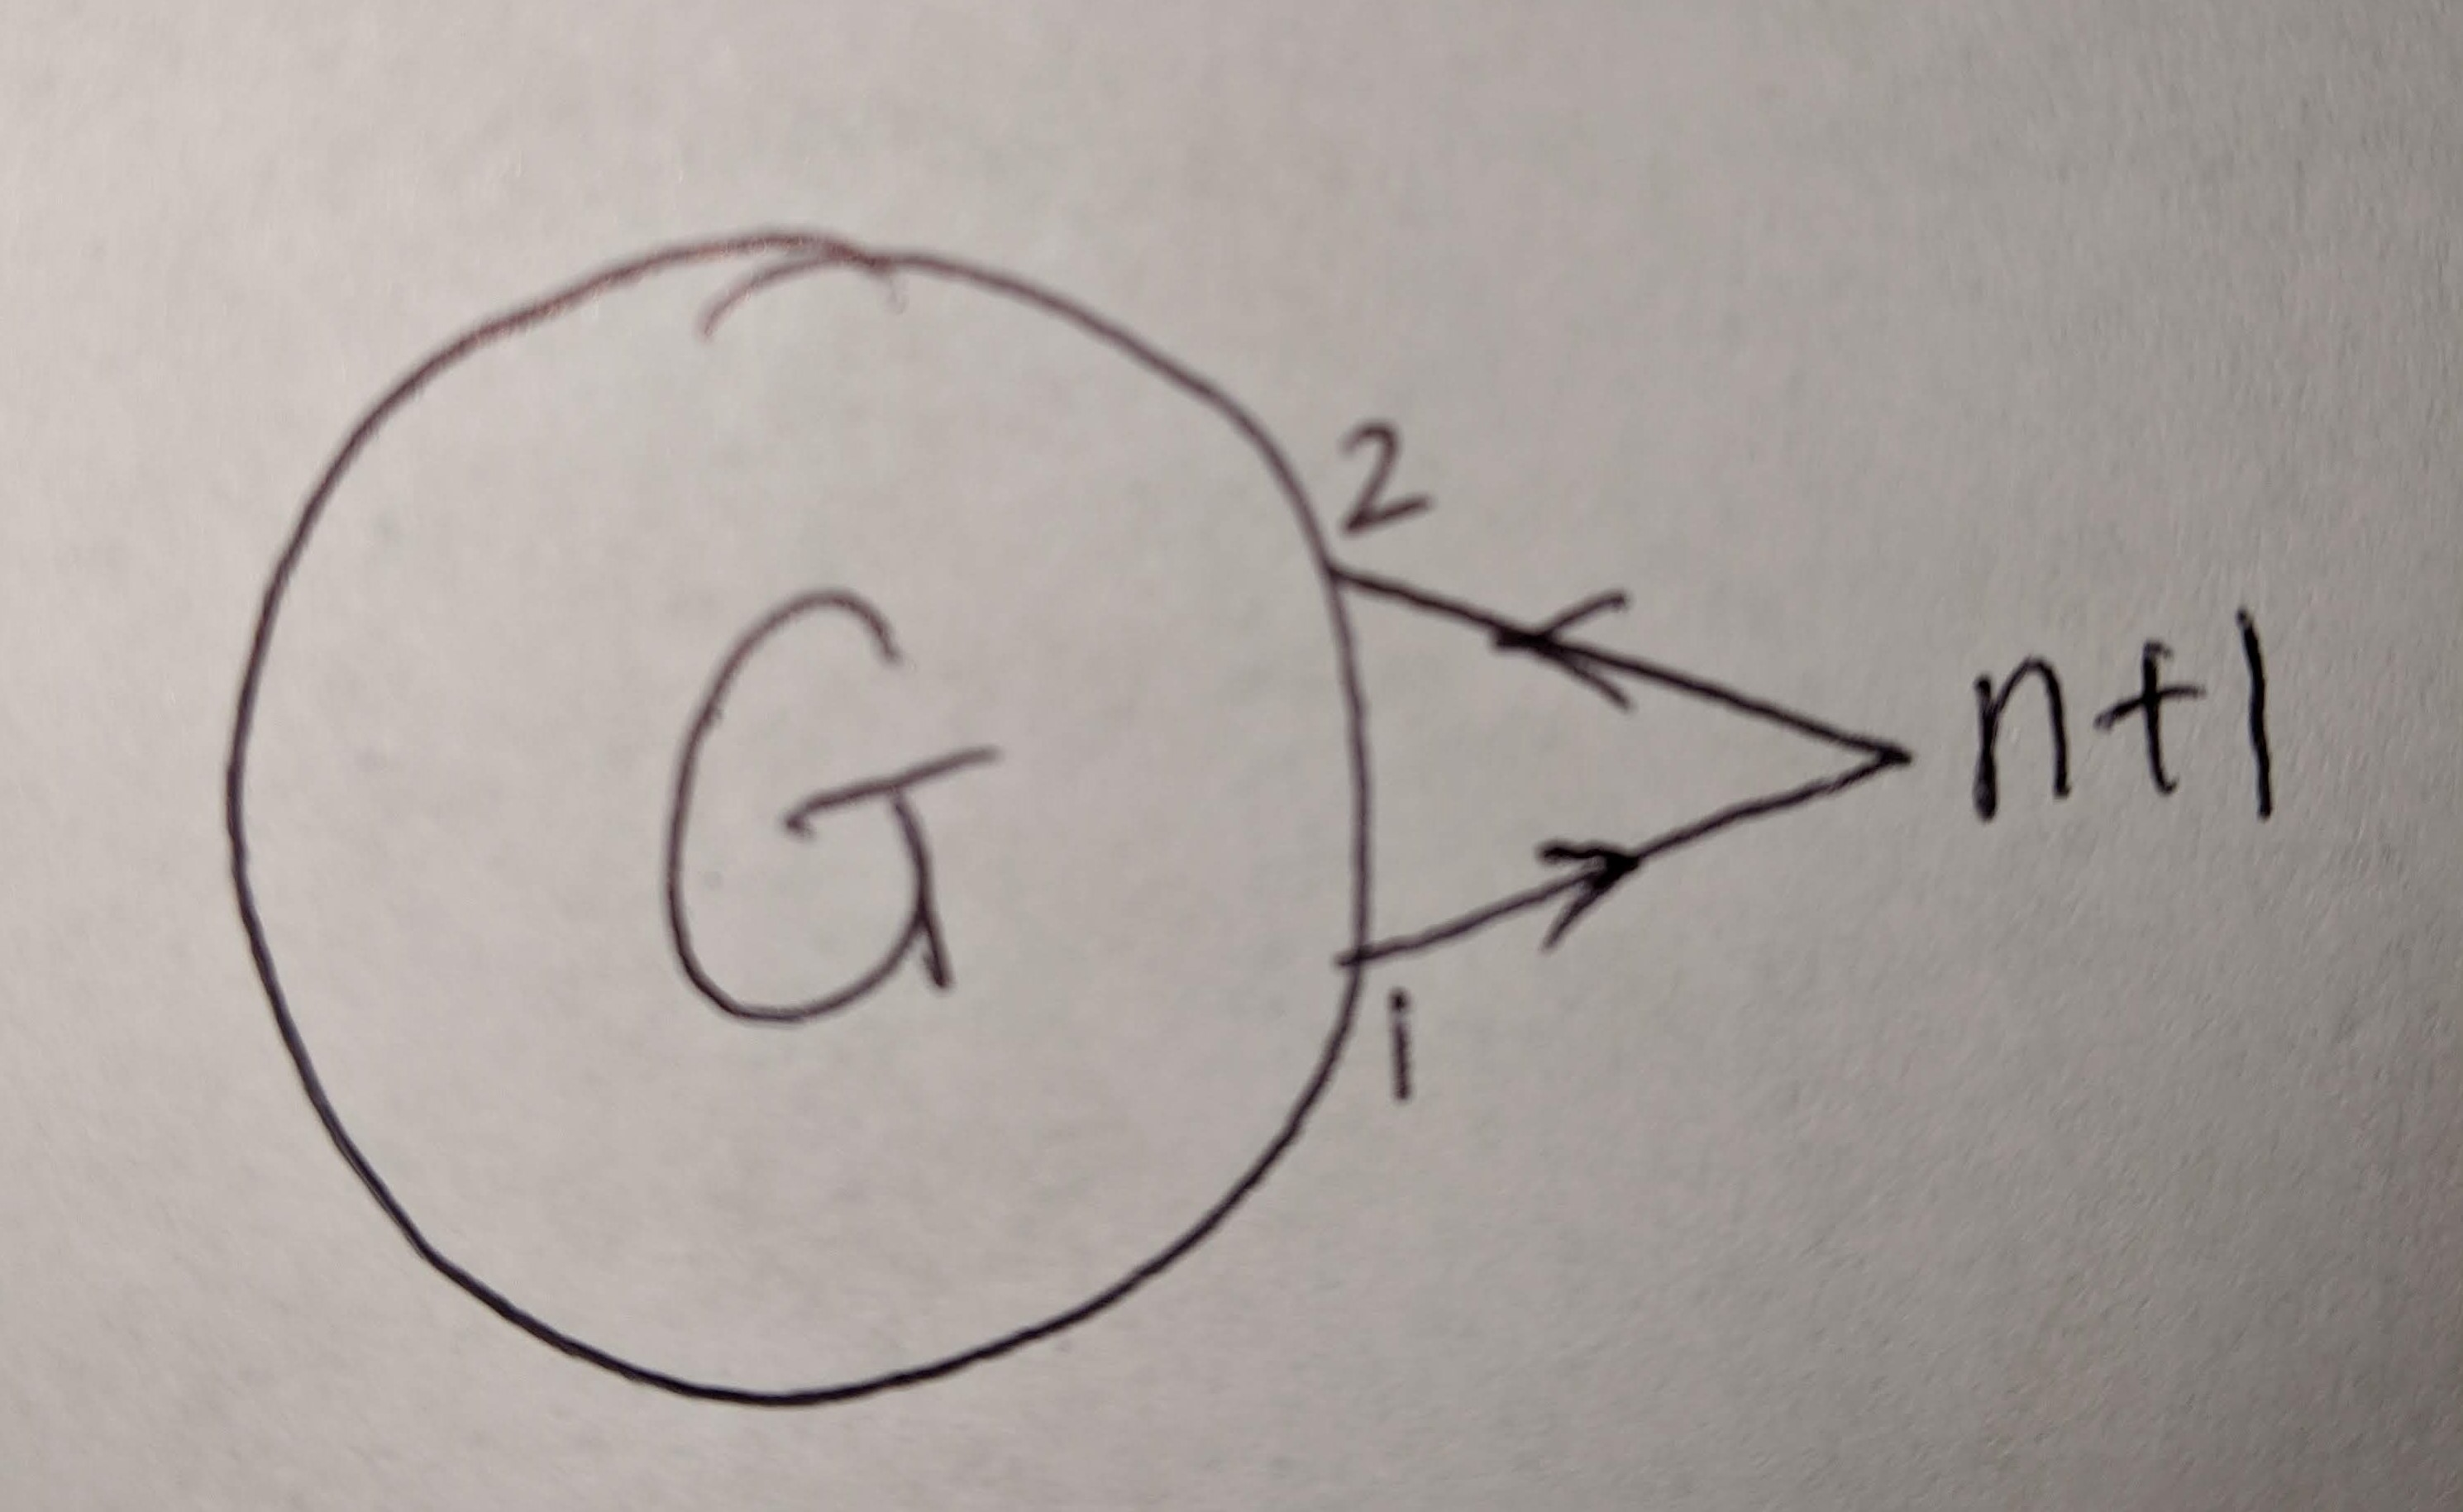
\includegraphics[scale=0.025]{graph1_1.jpg}
\ethm

\bpf
Let $VH_1(G)$ be directed handle graph with 1 handle, and let $T$ be a spanning tree in $VH_1(G)$. Suppose $T$ is rooted at vertex $v_1\in V(G)$. Let $e$ be the inflow edge. Then, there are two cases.\\
Case 1. $e\notin VH_1(G)$. Then the number of spanning tree is $\tau(G)$ by \Cref{bij_count}.\\
Case 2. $e \in VH_1(G)$. Then, since there does not exist a path in $G$ between node 1 and 2 by \Cref{symhandle}, the number of spanning tree is $\tau_{(1)(2)}(G)$.\\
Therefore, the total number of subgraphs of $VH_1(G)$ is  $$ \tau (VH_1(G))_1 = \tau(G)+\tau_{(1)(2)}(G)$$ .
\epf

\bthm
{\bf (Rooted at 2)}
Let $VH_1(G)$ be directed handle graph with 1 handle, and let $T$ be a spanning tree in $VH_1(G)$. If $T$ is rooted at vertex $v_2\in V(G)$ as shown in the picture below,
then the total number of subgraphs of $VH_1(G)$ is  \[
 \tau (VH_1(G))_2 = \tau(G)
\]
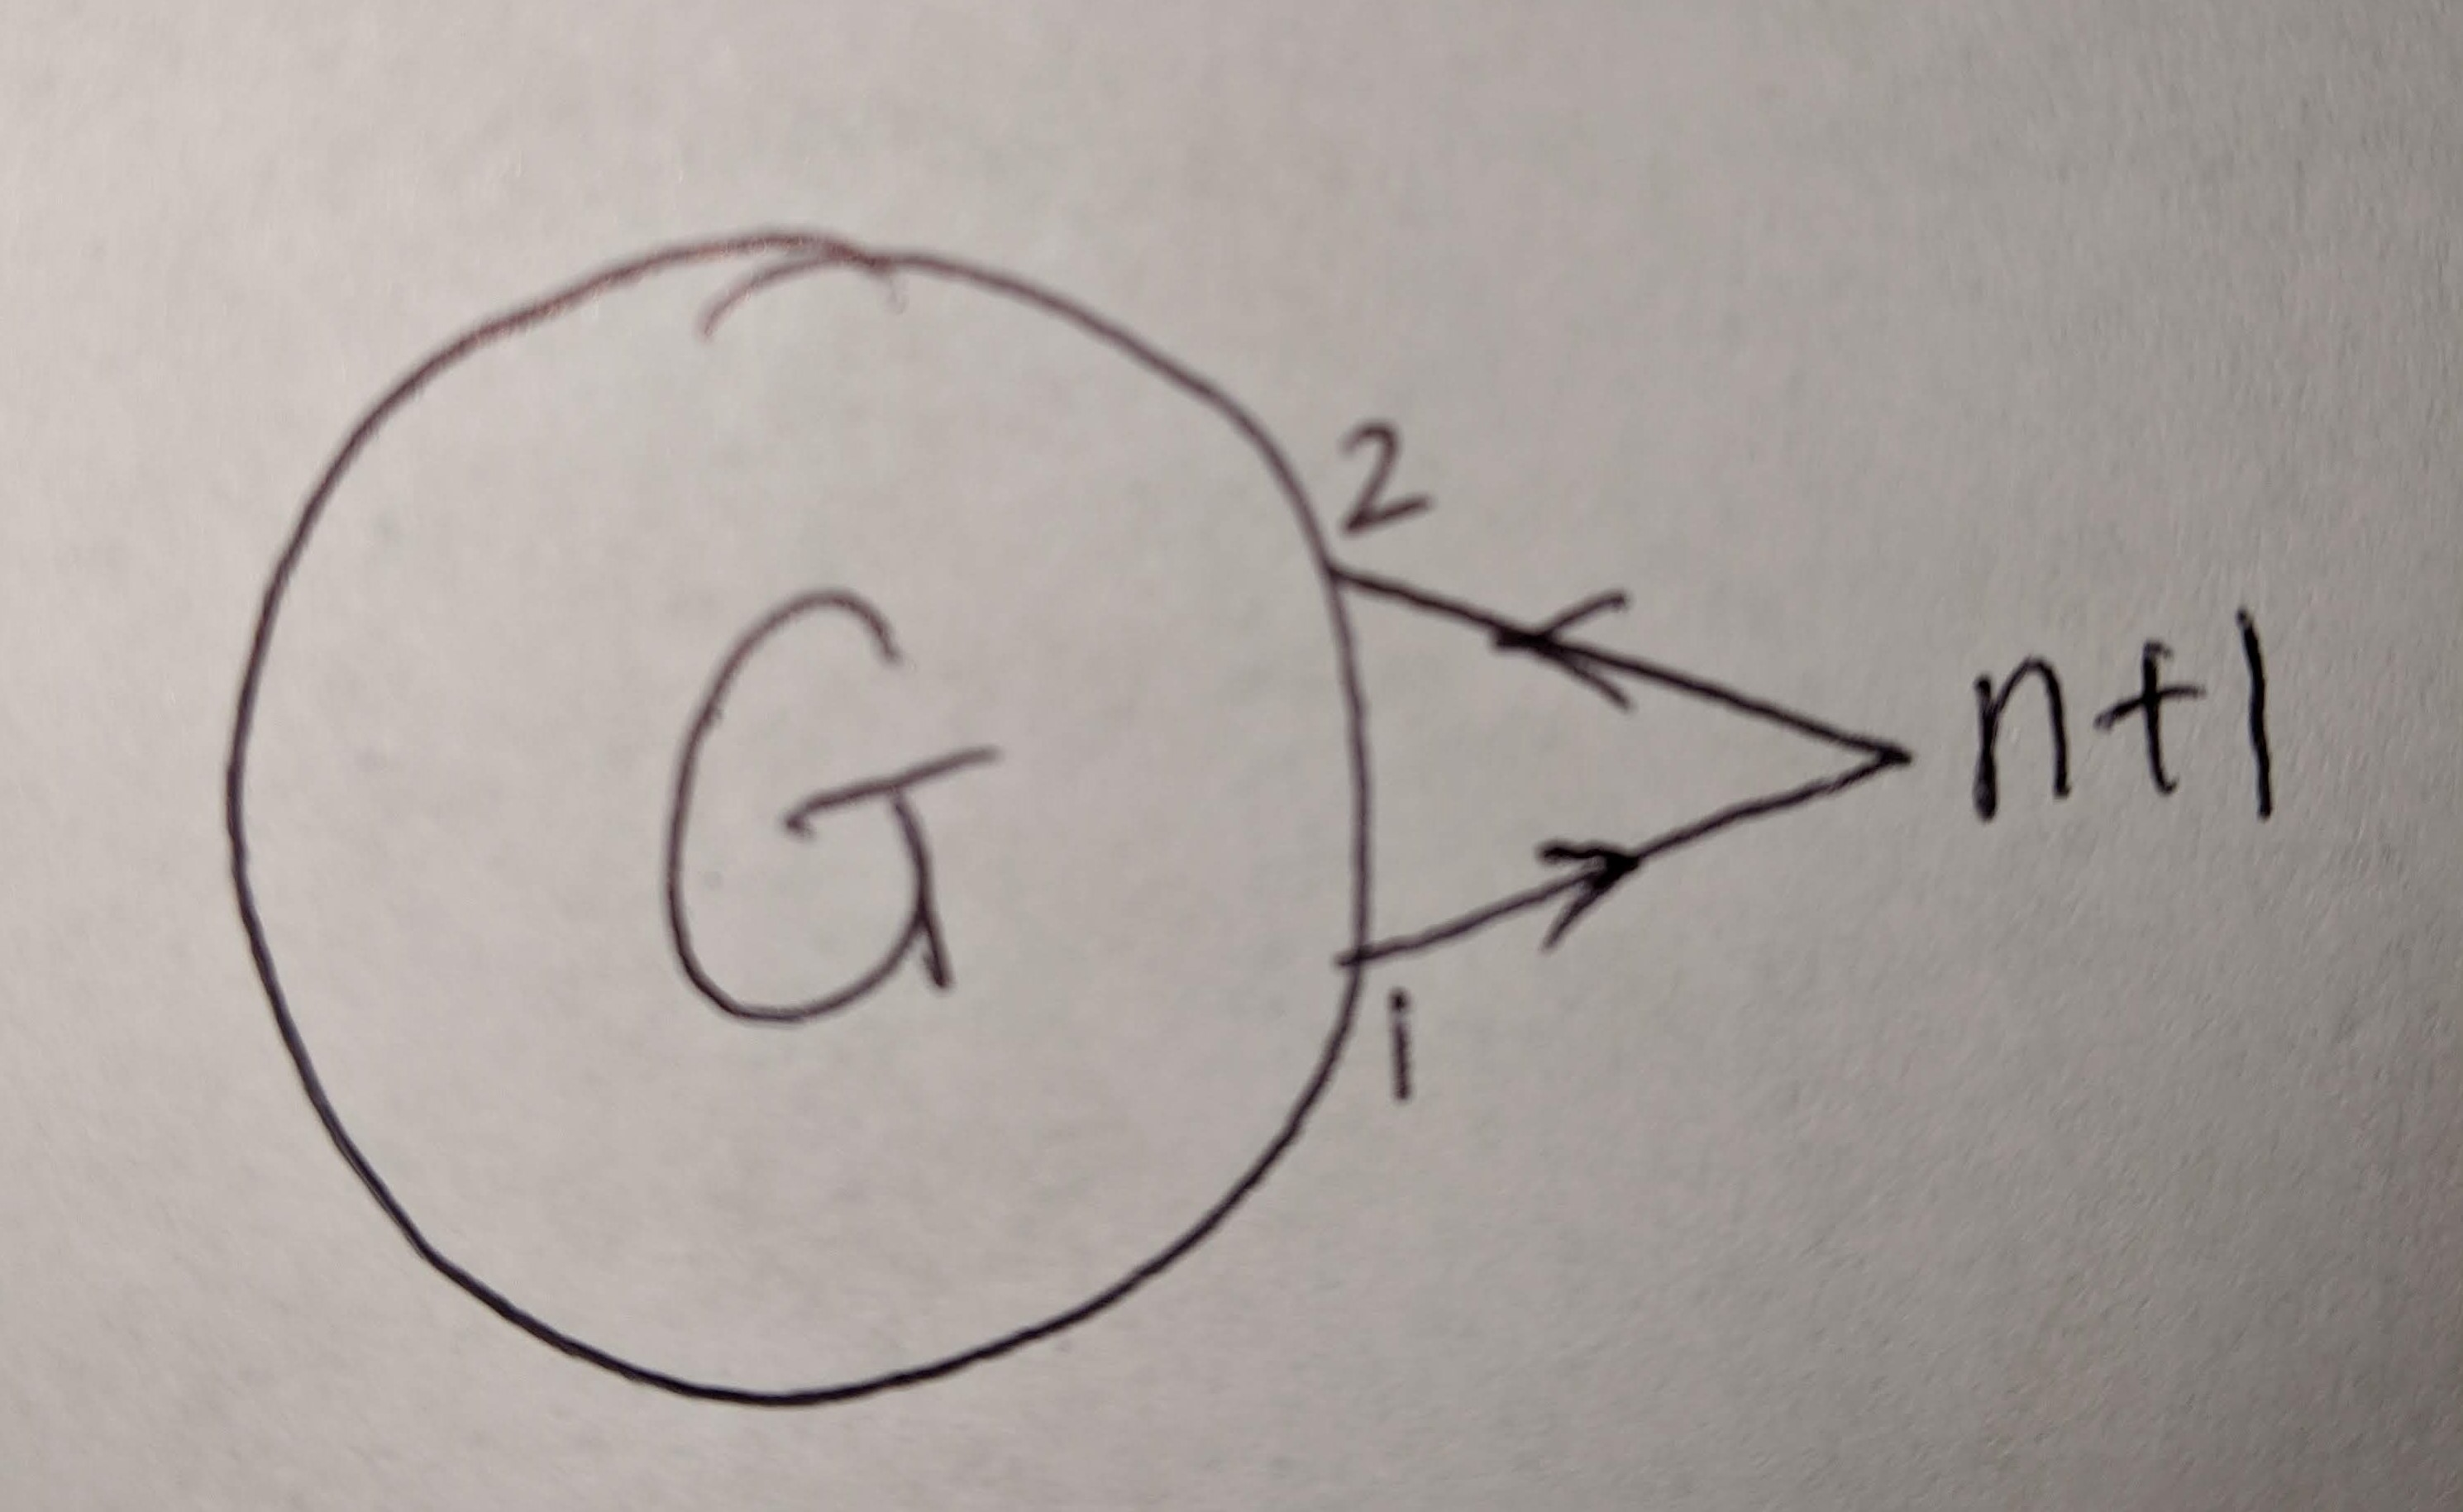
\includegraphics[scale=0.025]{graph1_1.jpg}
\ethm

\bpf
Let $VH_1(G)$ be directed handle graph with 1 handles, and let $T$ be a spanning tree in $VH_1(G)$. Suppose $T$ is rooted at vertex $v_2\in V(G)$. Then the inflow edge $e\notin VH_1(G)$. Then the total number of subgraphs of $VH_1(G)$ is  $ \tau (VH_1(G))_2 = \tau(G)$ by \Cref{bij_count}.
\epf

\bthm
{\bf (Rooted at 0)}
Let $VH_1(G)$ be directed handle graph with 1 handle, and let $T$ be a spanning tree in $VH_1(G)$. If $T$ is rooted at vertex $v_0\in V(G)$ as shown in the picture below, where $v_0$ is neither the outflow vertex nor the inflow vertex of the handle, 
then the total number of subgraphs of $VH_1(G)$ is  \[
 \tau (VH_1(G))_0 = \tau(G)+\tau_{(01)(2)}(G) 
\]
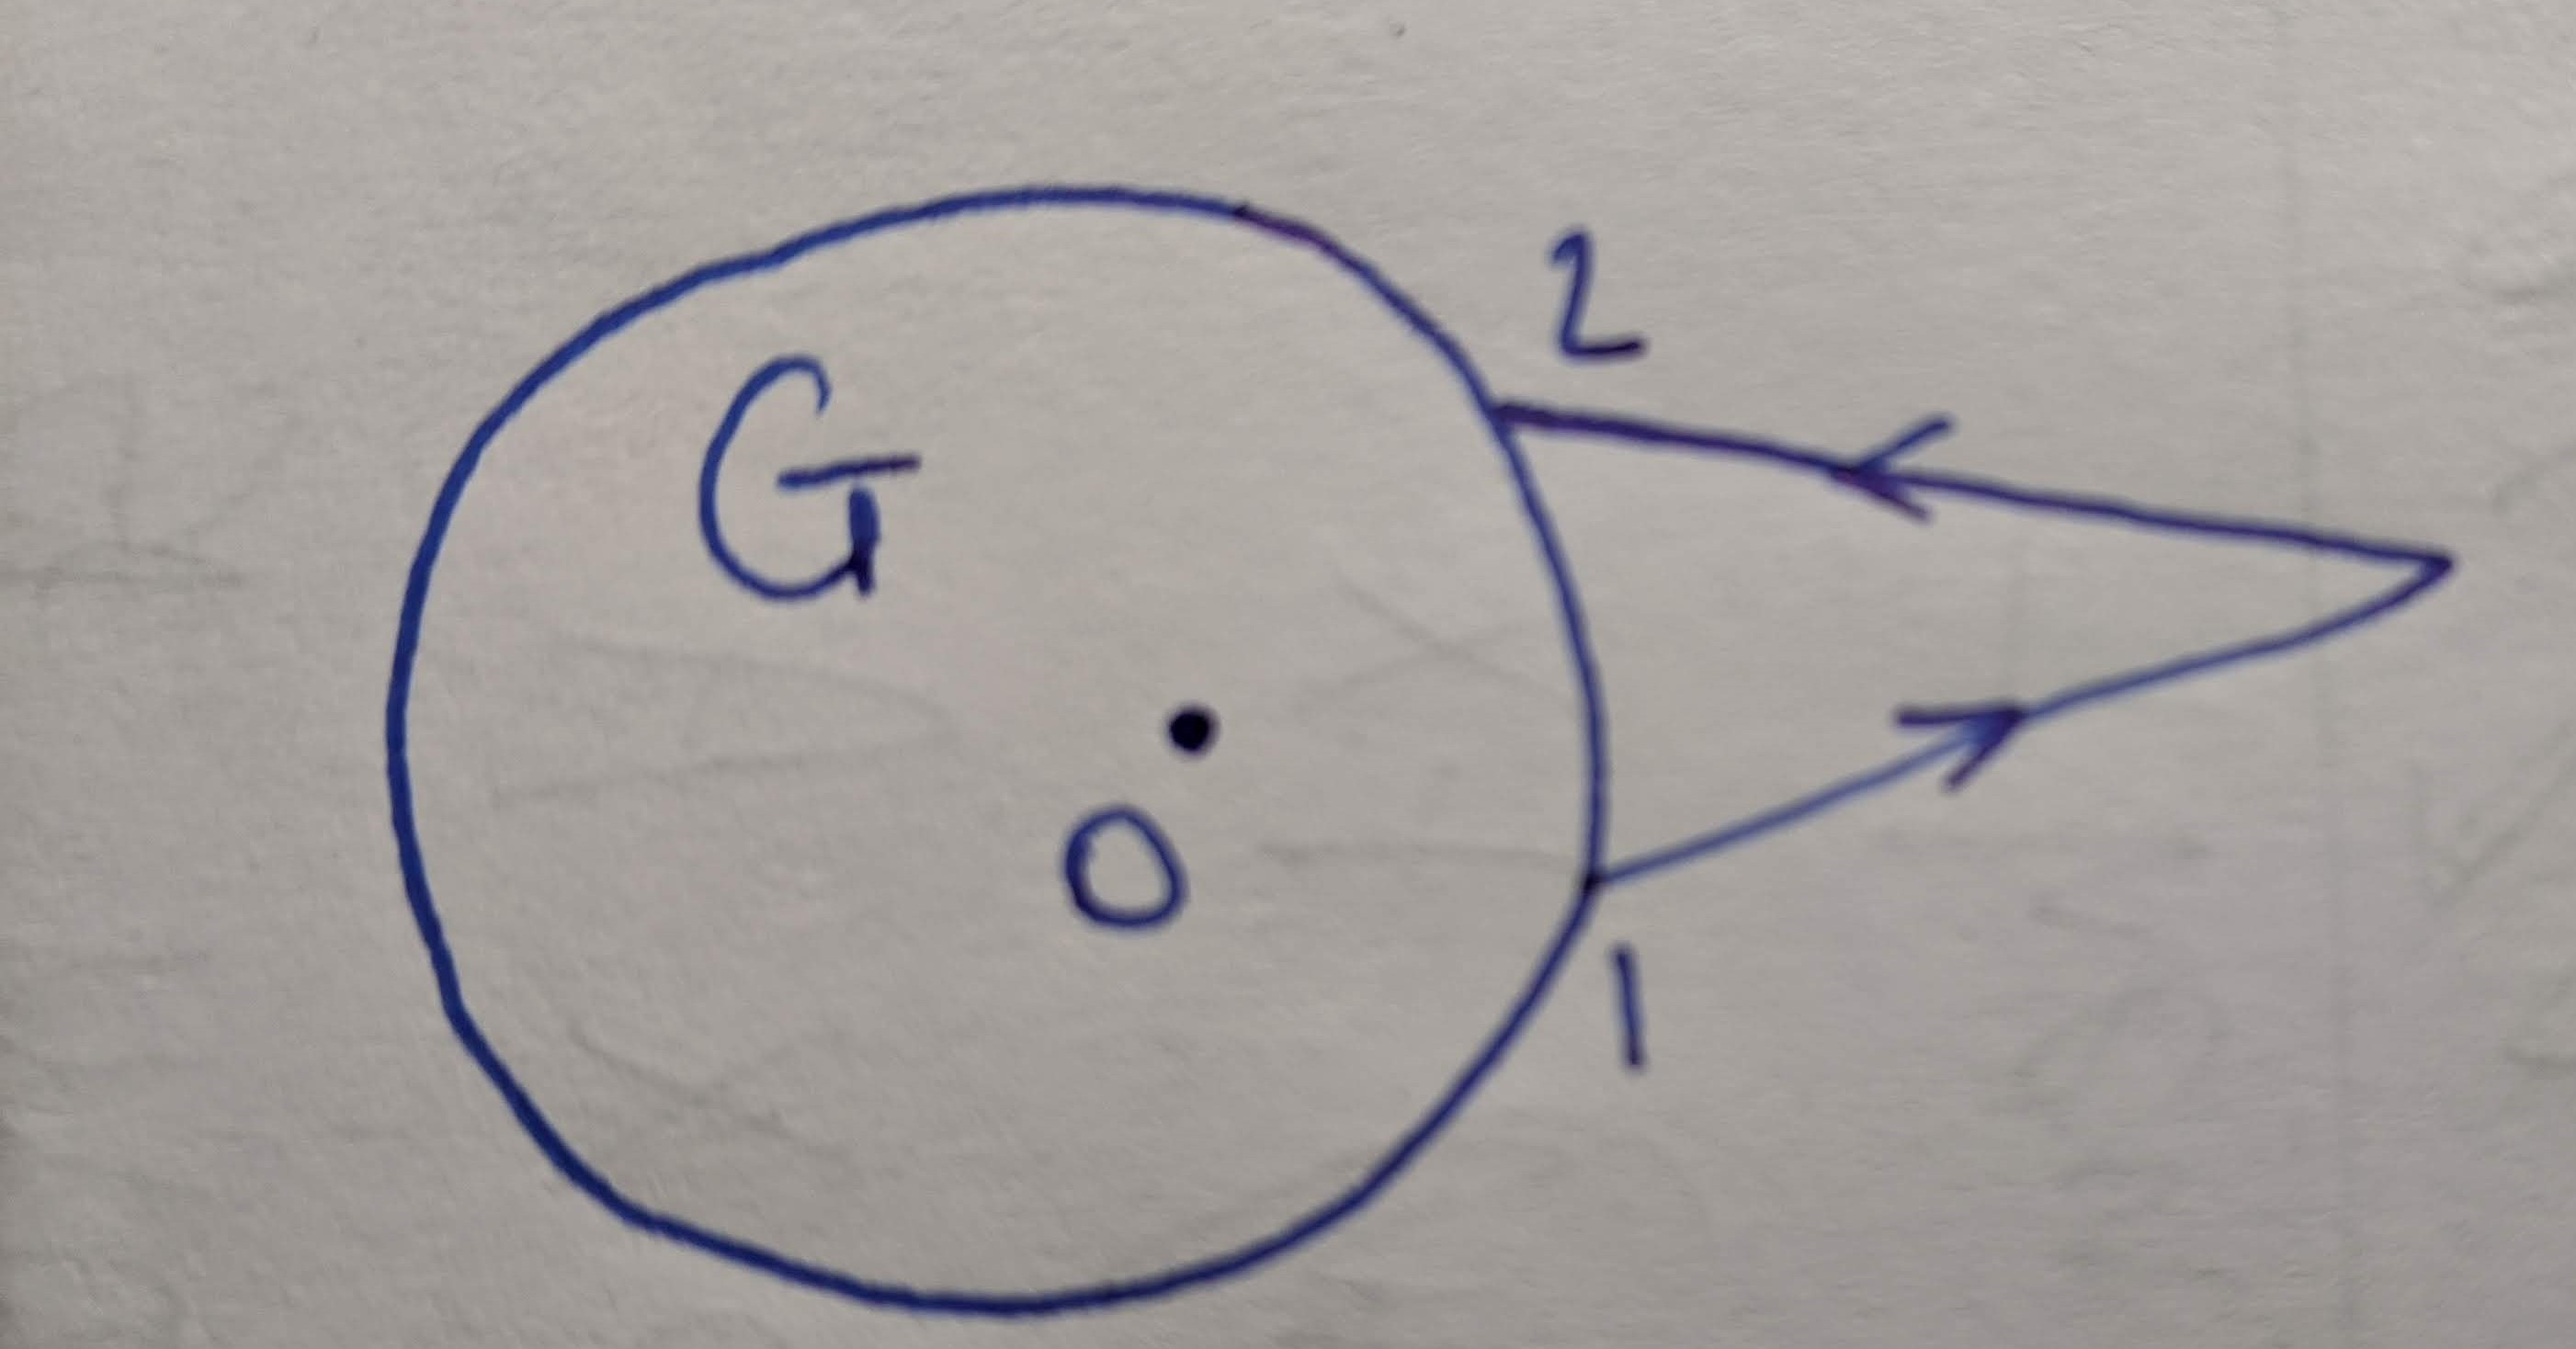
\includegraphics[scale=0.025]{graph1_0.jpg}
\ethm

\bpf
Let $VH_1(G)$ be directed handle graph with 1 handle, and let $T$ be a spanning tree in $VH_1(G)$. If $T$ is rooted at vertex $v_0\in V(G)$. Let $e$ be the inflow edge. Then, there are two cases.

Case 1. $e\notin VH_1(G)$. Then the number of spanning tree is $\tau(G)$ by \Cref{bij_count}.

Case 2. $e \in VH_1(G)$. Then, since there does not exist a path between node 1 and 2 by \cref{symhandle}, the number of spanning tree is $\tau_{(01)(2)}(G)$.

Therefore, the total number of subgraphs of $VH_1(G)$ is  $$ \tau (VH_1(G))_0 = \tau(G)+\tau_{(01)(2)}(G)$$ .
\epf


\section{Two Handles.}
\blm
\label{addedW}
Let $H=\{ (v_1,...,v_k), (v_{k+1},v_{k+2},...,v_p)\}$. Then $$T_{(v_1,...,v_k), (v_{k+1},v_{k+2},...,v_p)}(G)=T_{(v_1,...,v_k,w)(v_{k+1},v_{k+2},...,v_p)}(G)+T_{(v_1,...,v_k)(v_{k+1},v_{k+2},...,v_p,w)}(G)$$
for $w\in V(G)$ and neither $(v_1,...,v_k,w)$ nor $(v_{k+1},v_{k+2},...,v_p,w)$ form cycles.
\elm

\bpf
Let $H=\{ (v_1,...,v_k), (v_{k+1},v_{k+2},...,v_p)\}$, and $w\in V(G)$ and neither $(v_1,...,v_k,w)$ nor $(v_{k+1},v_{k+2},...,v_p,w)$ form cycles in $G$.
Since neither $(v_1,...,v_k,w)$ nor $(v_{k+1},v_{k+2},...,v_p,w)$  form cycles, there are two cases. \\
Case 1. $w$ is connected to $(v_1,...,v_k)$. Then the number of spanning tree is $T_{(v_1,...,v_k,w)(v_{k+1},v_{k+2},...,v_p)}(G)$. \\
Case 1. $w$ is connected to $(v_{k+1},v_{k+2},...,v_p)$. Then the number of spanning tree is $T_{(v_1,...,v_k)(v_{k+1},v_{k+2},...,v_p,w)}(G)$. \\
So, total number of spanning trees is $T_{(v_1,...,v_k), (v_{k+1},v_{k+2},...,v_p)}(G)=T_{(v_1,...,v_k,w)(v_{k+1},v_{k+2},...,v_p)}(G)+T_{(v_1,...,v_k)(v_{k+1},v_{k+2},...,v_p,w)}(G)$.
\epf

\bthm
{\bf (Rooted at 1)}
Let $VH_2(G)$ be directed handle graph with 2 handles, and let $T$ be a spanning tree in $VH_2(G)$. If $T$ is rooted at vertex $v_1\in V(G)$ as shown in the picture below,
then the total number of subgraphs of $VH_2(G)$ is  
\begin{equation*}
    \begin{split}
        \tau(VH_2(G))_1 &= \tau(G)+\tau_{(1)(2)}(G)+\tau_{(3)(4)}(G)+
 \tau_{(13)(2)(4)}(G)+\tau_{(1)(23)(4)}(G)  \\
 & = \tau(G)+\tau_{(1)(2)}(G)+\tau_{(3)(4)}(G)+
 \tau_{(1)(2)(4)}(G)-\tau_{(1)(2)(34)}(G)
    \end{split}
\end{equation*}

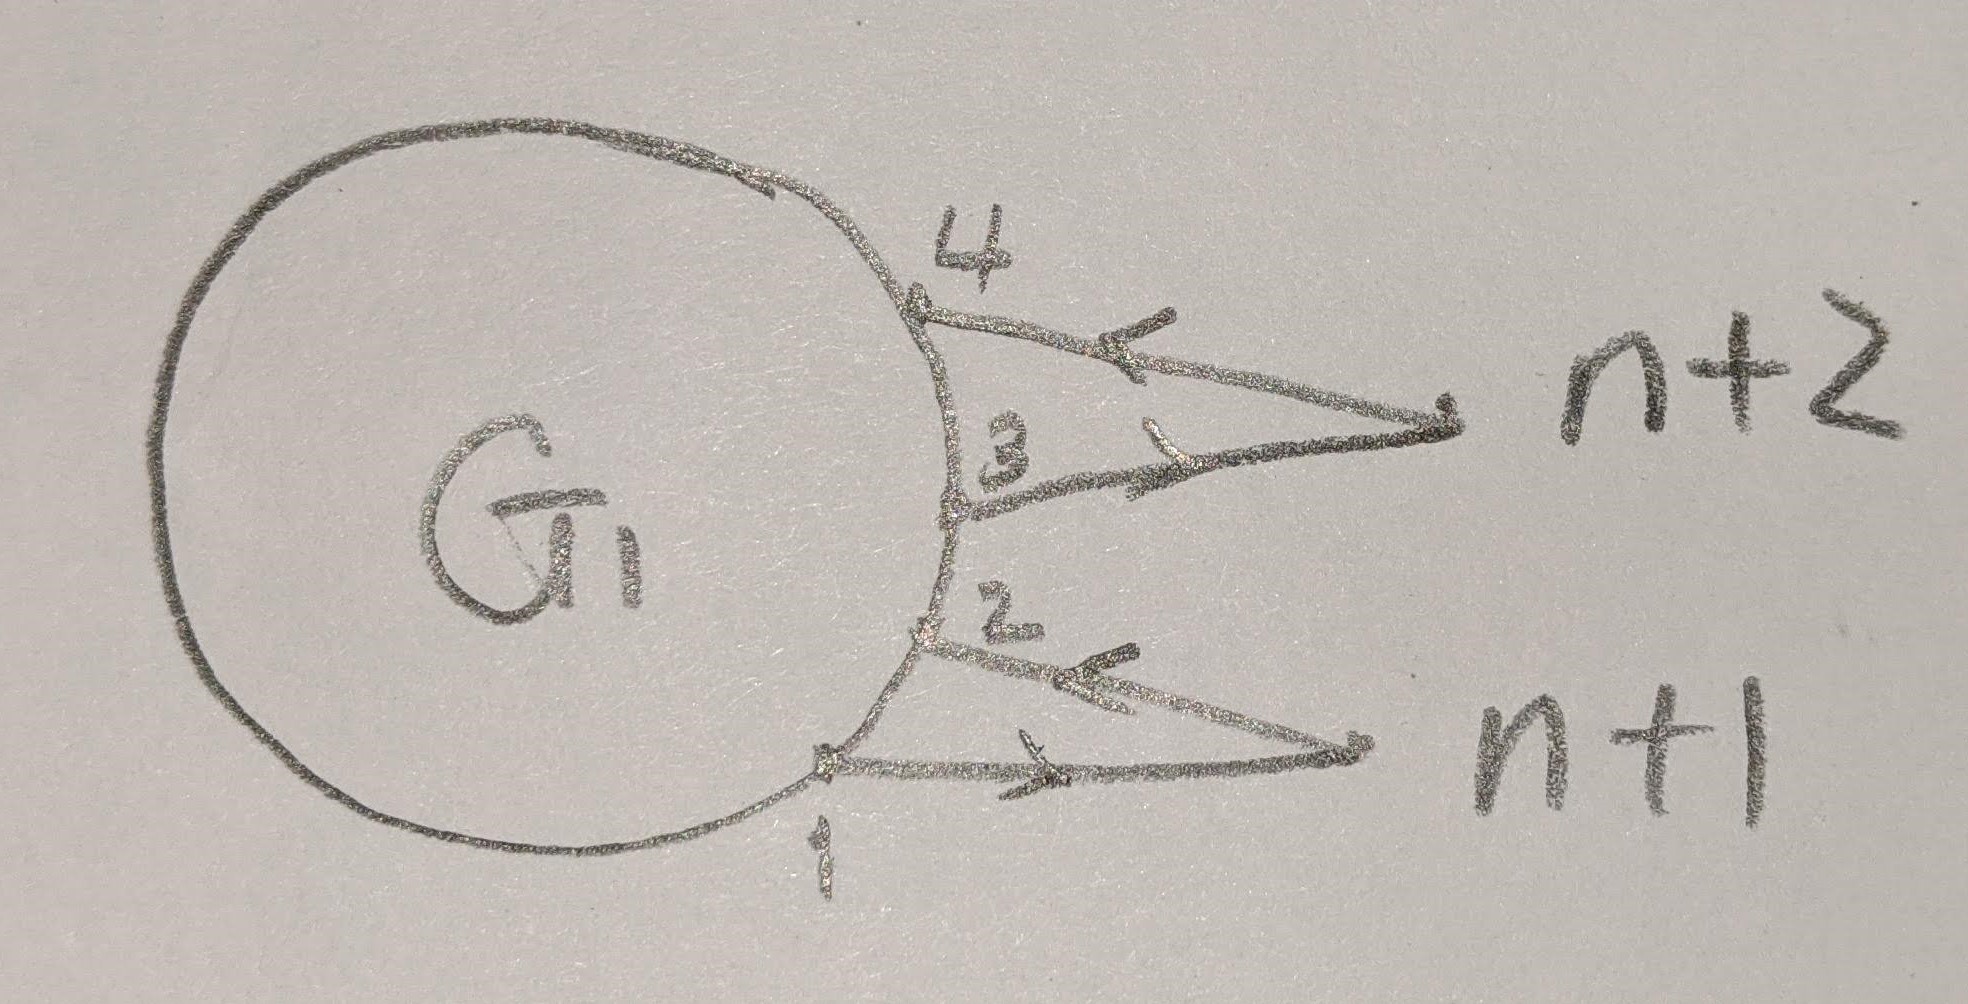
\includegraphics[scale=0.05]{graph2_1.jpg}
\ethm

\bpf
Let $VH_2(G)$ be directed handle graph with 2 handles, and let $T$ be a spanning tree in $VH_2(G)$. Suppose $T$ is rooted at vertex $v_1\in V(G)$.Let $e_1$ be the inflow edge to node 2, and $e_2$ be the inflow edge to node 4. There are three cases.\\
Case 1. $e_1\notin VH_2(G)$ and $e_2\notin VH_2(G)$. Then $\tau(VH_2(G))_1=\tau(G)$ by \Cref{bij_count}.\\
Case 2. $e_1\in VH_2(G)$ and $e_2\notin VH_2(G)$. By \Cref{bij_count} and \Cref{addedW}, $$\tau(VH_2(G))_1 = \tau_{(1)(2)}(G)$$
Case 3. $e_1\notin VH(G)$ and $e_2\in VH(G)$.Similar to Case 2,  $$\tau(VH_2(G))_1 = \tau_{(3)(4)}(G)$$
Case 4. $e_1\in VH(G)$ and $e_2\in VH(G)$.\\
By \Cref{symhandle}, there is not exists a path between $v_1$ and $v_2$, nor a path between  $v_3$ and $v_4$. So, by \Cref{addedW}
$$\tau(VH_2(G))_1 = \tau_{(13)(2)(4)}(G)+\tau_{(1)(23)(4)}(G) = \tau_{(1)(2)(4)}(G)-\tau_{(1)(2)(34)}(G)$$
Therefore, the total number of subgraphs of $VH(G)$ is \[
 \tau(VH_2(G))_1 = \tau(G)+\tau_{(1)(2)}(G)+\tau_{(3)(4)}(G)+
 \tau_{(13)(2)(4)}(G)+\tau_{(1)(23)(4)}(G) 
\]

\epf

\bthm
{\bf (Rooted at 2)}
Let $VH_2(G)$ be directed handle graph with 2 handles, and let $T$ be a spanning tree in $VH_2(G)$. If $T$ is rooted at vertex $v_2\in V(G)$ as shown in the picture below,
then the total number of subgraphs of $VH(G)$ is  \[
\tau(VH_2(G))_2 = \tau(G) + \tau_{(3)(4)}(G)
\]
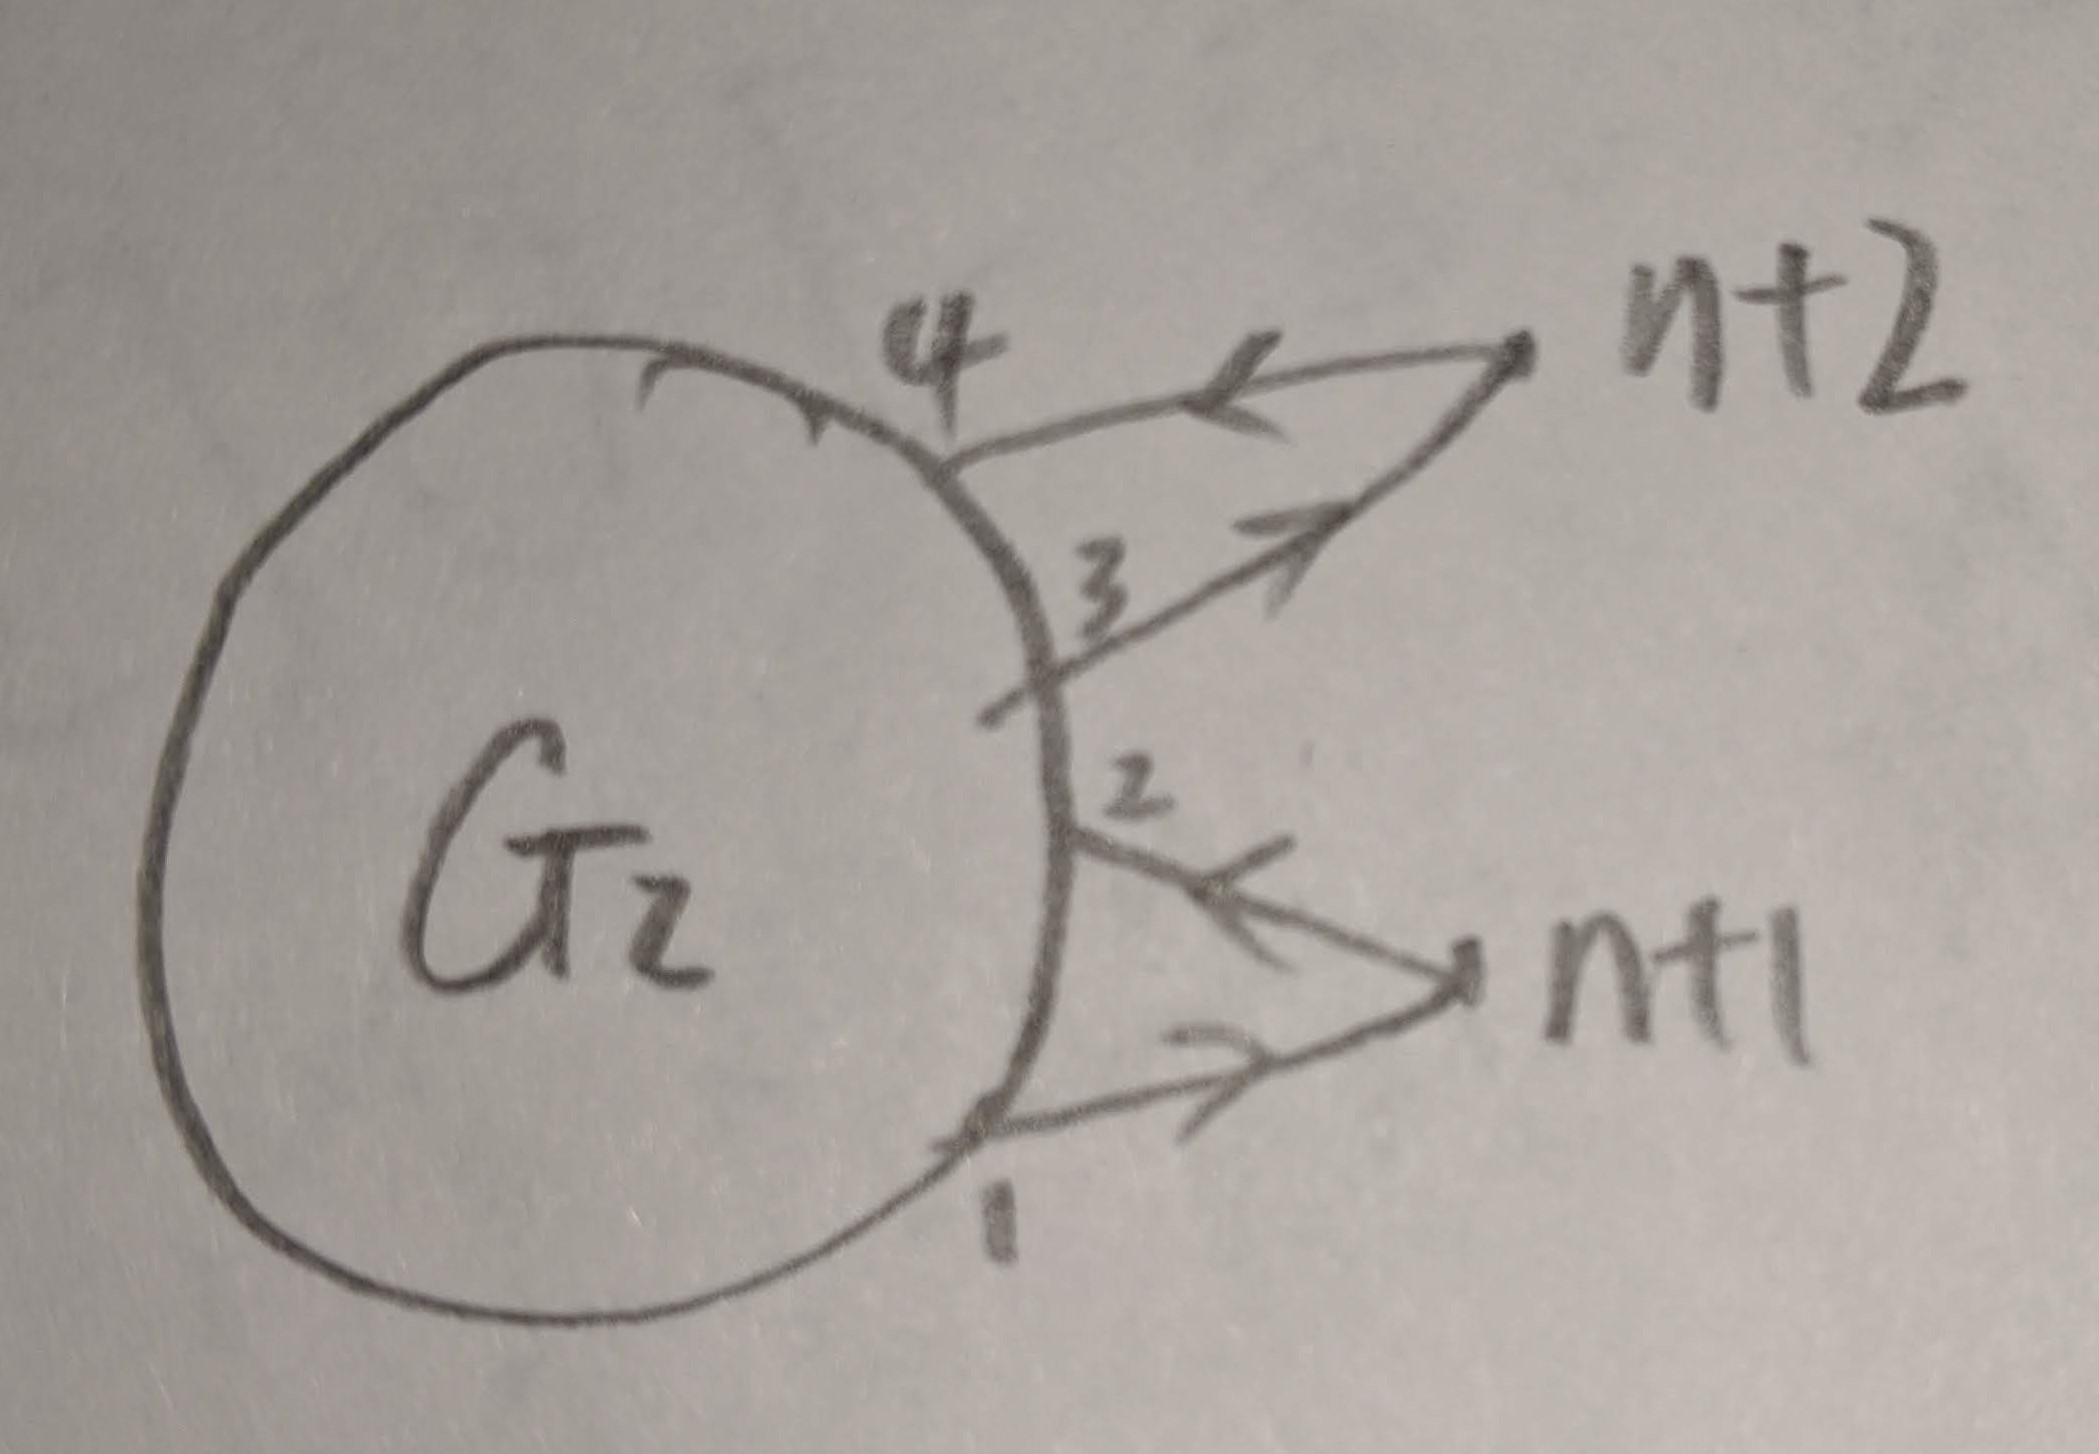
\includegraphics[scale=0.05]{graph2_2.jpg}
\ethm

\bpf
Let $VH_2(G)$ be directed handle graph with 2 handles, and let $T$ be a spanning tree in $VH_2(G)$. Suppose $T$ is rooted at vertex $v_2\in V(G)$. Let the inflow edge to $v_2$ be $e_1$ and the inflow edge to $v_4$ be $e_2$.\\
Case 1. $e_1 \notin T$ and $e_2 \notin T$.\\
Then $\tau(VH_2(G))_2=\tau(G)$ by \Cref{bij_count}.\\
Case 2. $e_1 \in T$.\\
This contradicts with $T$ is rooted at $e_2$.\\
Case 3. $e_1\notin T$ and $e_2 \in T$.\\
By \Cref{symhandle}, there does not exist a path between $v_3$ and $v_4$. Then by \Cref{bij_count}, $\tau(VH_2(G))_2 = \tau_{(3)(4)}(G)$\\
Therefore, the total number of subgraphs of $VH(G)$ is \[
\tau(VH_2(G))_2 = \tau(G) + \tau_{(3)(4)}(G)
\]
\epf

\bthm
{\bf (Rooted at 3)}
Let $VH_2(G)$ be directed handle graph with 2 handles, and let $T$ be a spanning tree in $VH_2(G)$. If $T$ is rooted at vertex $v_3\in V(G)$ as shown in the picture below,
then the total number of subgraphs of $VH_2(G)$ is  
\begin{equation*}
    \begin{split}
        \tau(VH_2(G))_3 &= \tau(G)+\tau_{(1)(2)}(G)+\tau_{(3)(4)}(G)+
 \tau_{(13)(2)(4)}(G)+\tau_{(3)(2)(14)}(G)  \\
 &= \tau(G)+\tau_{(1)(2)}(G)+\tau_{(3)(4)}(G)+
 \tau_{(3)(2)(4)}(G)-\tau_{(3)(12)(4)}(G)
    \end{split}
\end{equation*}

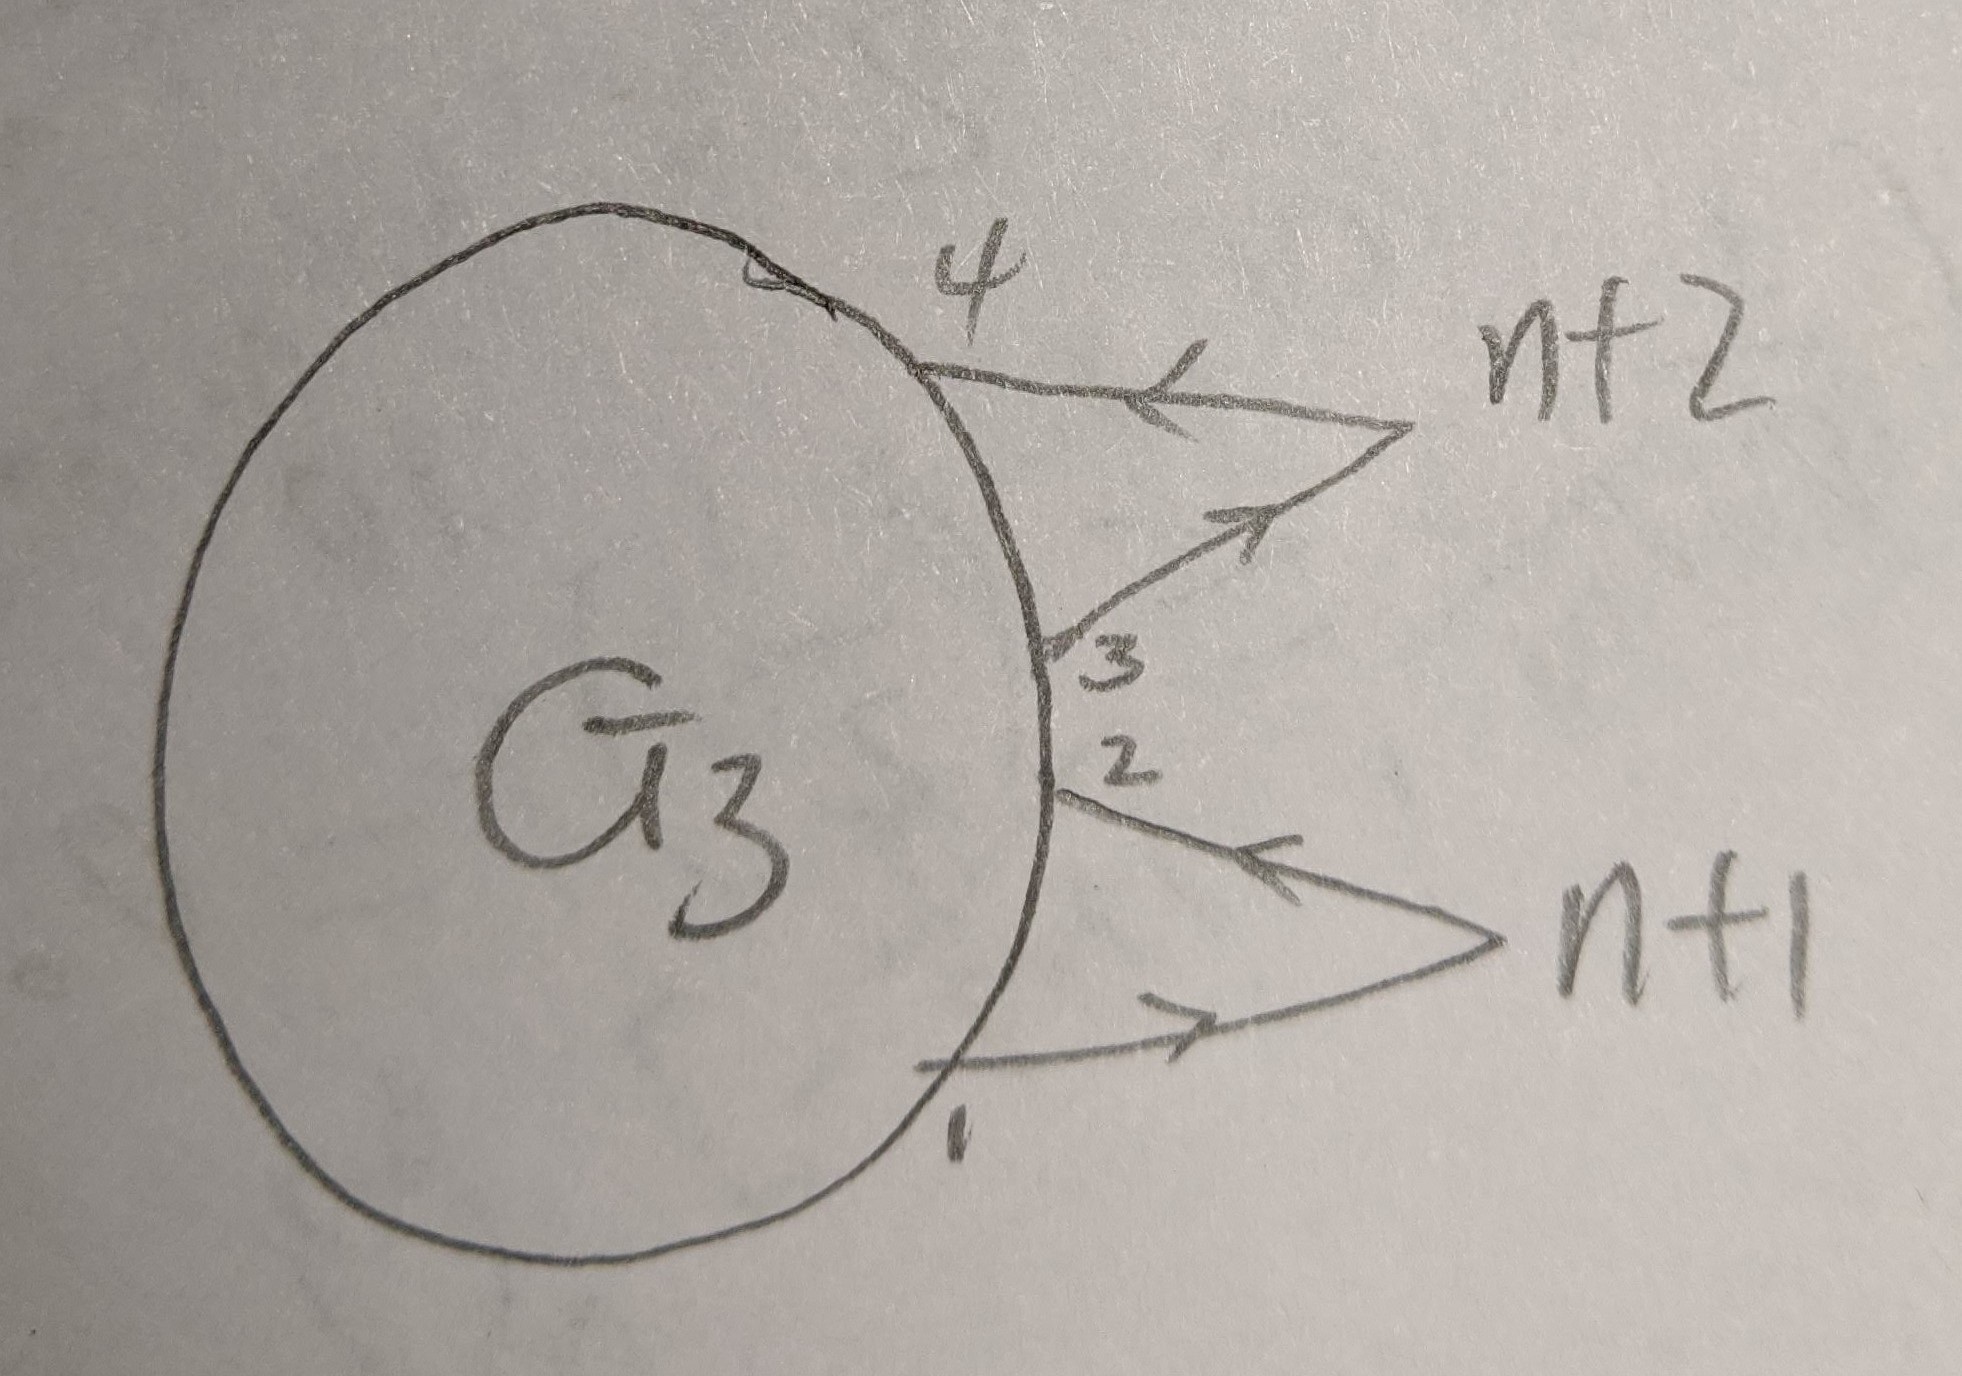
\includegraphics[scale=0.05]{graph2_3.jpg}
\ethm

\bpf
%Let $VH_2(G)$ be directed handle graph with 2 handles, and let $T$ be a spanning tree in $VH_2(G)$. Suppose $T$ is rooted at vertex $v_3\in V(G)$.Let $e_1$ be the inflow edge to node 2, and $e_2$ be the inflow edge to node 4. There are three cases.\\
%Case 1. $e_1\notin VH_2(G)$ and $e_2\notin VH_2(G)$. Then $\tau(VH_2(G))_3=\tau(G)$ by \Cref{bij_count}.\\
%Case 2. $e_1\in VH_2(G)$ and $e_2\notin VH_2(G)$. By \Cref{bij_count} and \Cref{addedW}, $$\tau(VH_2(G))_1 = \tau_{(1)(2)}(G)$$
%Case 3. $e_1\notin VH(G)$ and $e_2\in VH(G)$.Similar to Case 2,  $$\tau(VH_2(G))_3 = \tau_{(3)(4)}(G)$$
%Case 4. $e_1\in VH(G)$ and $e_2\in VH(G)$.\\
%By \Cref{symhandle}, there is not exists a path between $v_1$ and $v_2$, nor a path between  $v_3$ and $v_4$. So, by \Cref{addedW}
%$$\tau(VH_2(G))_3 = \tau_{(13)(2)(4)}(G)+\tau_{(1)(23)(4)}(G) = \tau_{(1)(2)(4)}(G)-\tau_{(1)(2)(34)}(G)$$
%Therefore, the total number of subgraphs of $VH(G)$ is 
%\[\tau(VH_2(G))_3 = \tau(G)+\tau_{(1)(2)}(G)+\tau_{(3)(4)}(G)+\tau_{(1)(2)(4)}(G)-\tau_{(1)(2)(34)}(G)  \]
Since graph rooted at 3 is symmetric to graph rooted at 1, by swapping node 1 and 3, we have  $$\tau(VH_2(G))_3 =\tau(G)+\tau_{(1)(2)}(G)+\tau_{(3)(4)}(G)+
 \tau_{(13)(2)(4)}(G)+\tau_{(3)(2)(14)}(G)   $$
 
\epf

\bthm
{\bf (Rooted at 4)}
Let $VH_2(G)$ be directed handle graph with 2 handles, and let $T$ be a spanning tree in $VH_2(G)$. If $T$ is rooted at vertex $v_4\in V(G)$ as shown in the picture below,
then the total number of subgraphs of $VH(G)$ is  \[
\tau(VH_2(G))_4 = \tau(G) + \tau_{(1)(2)}(G)
\]
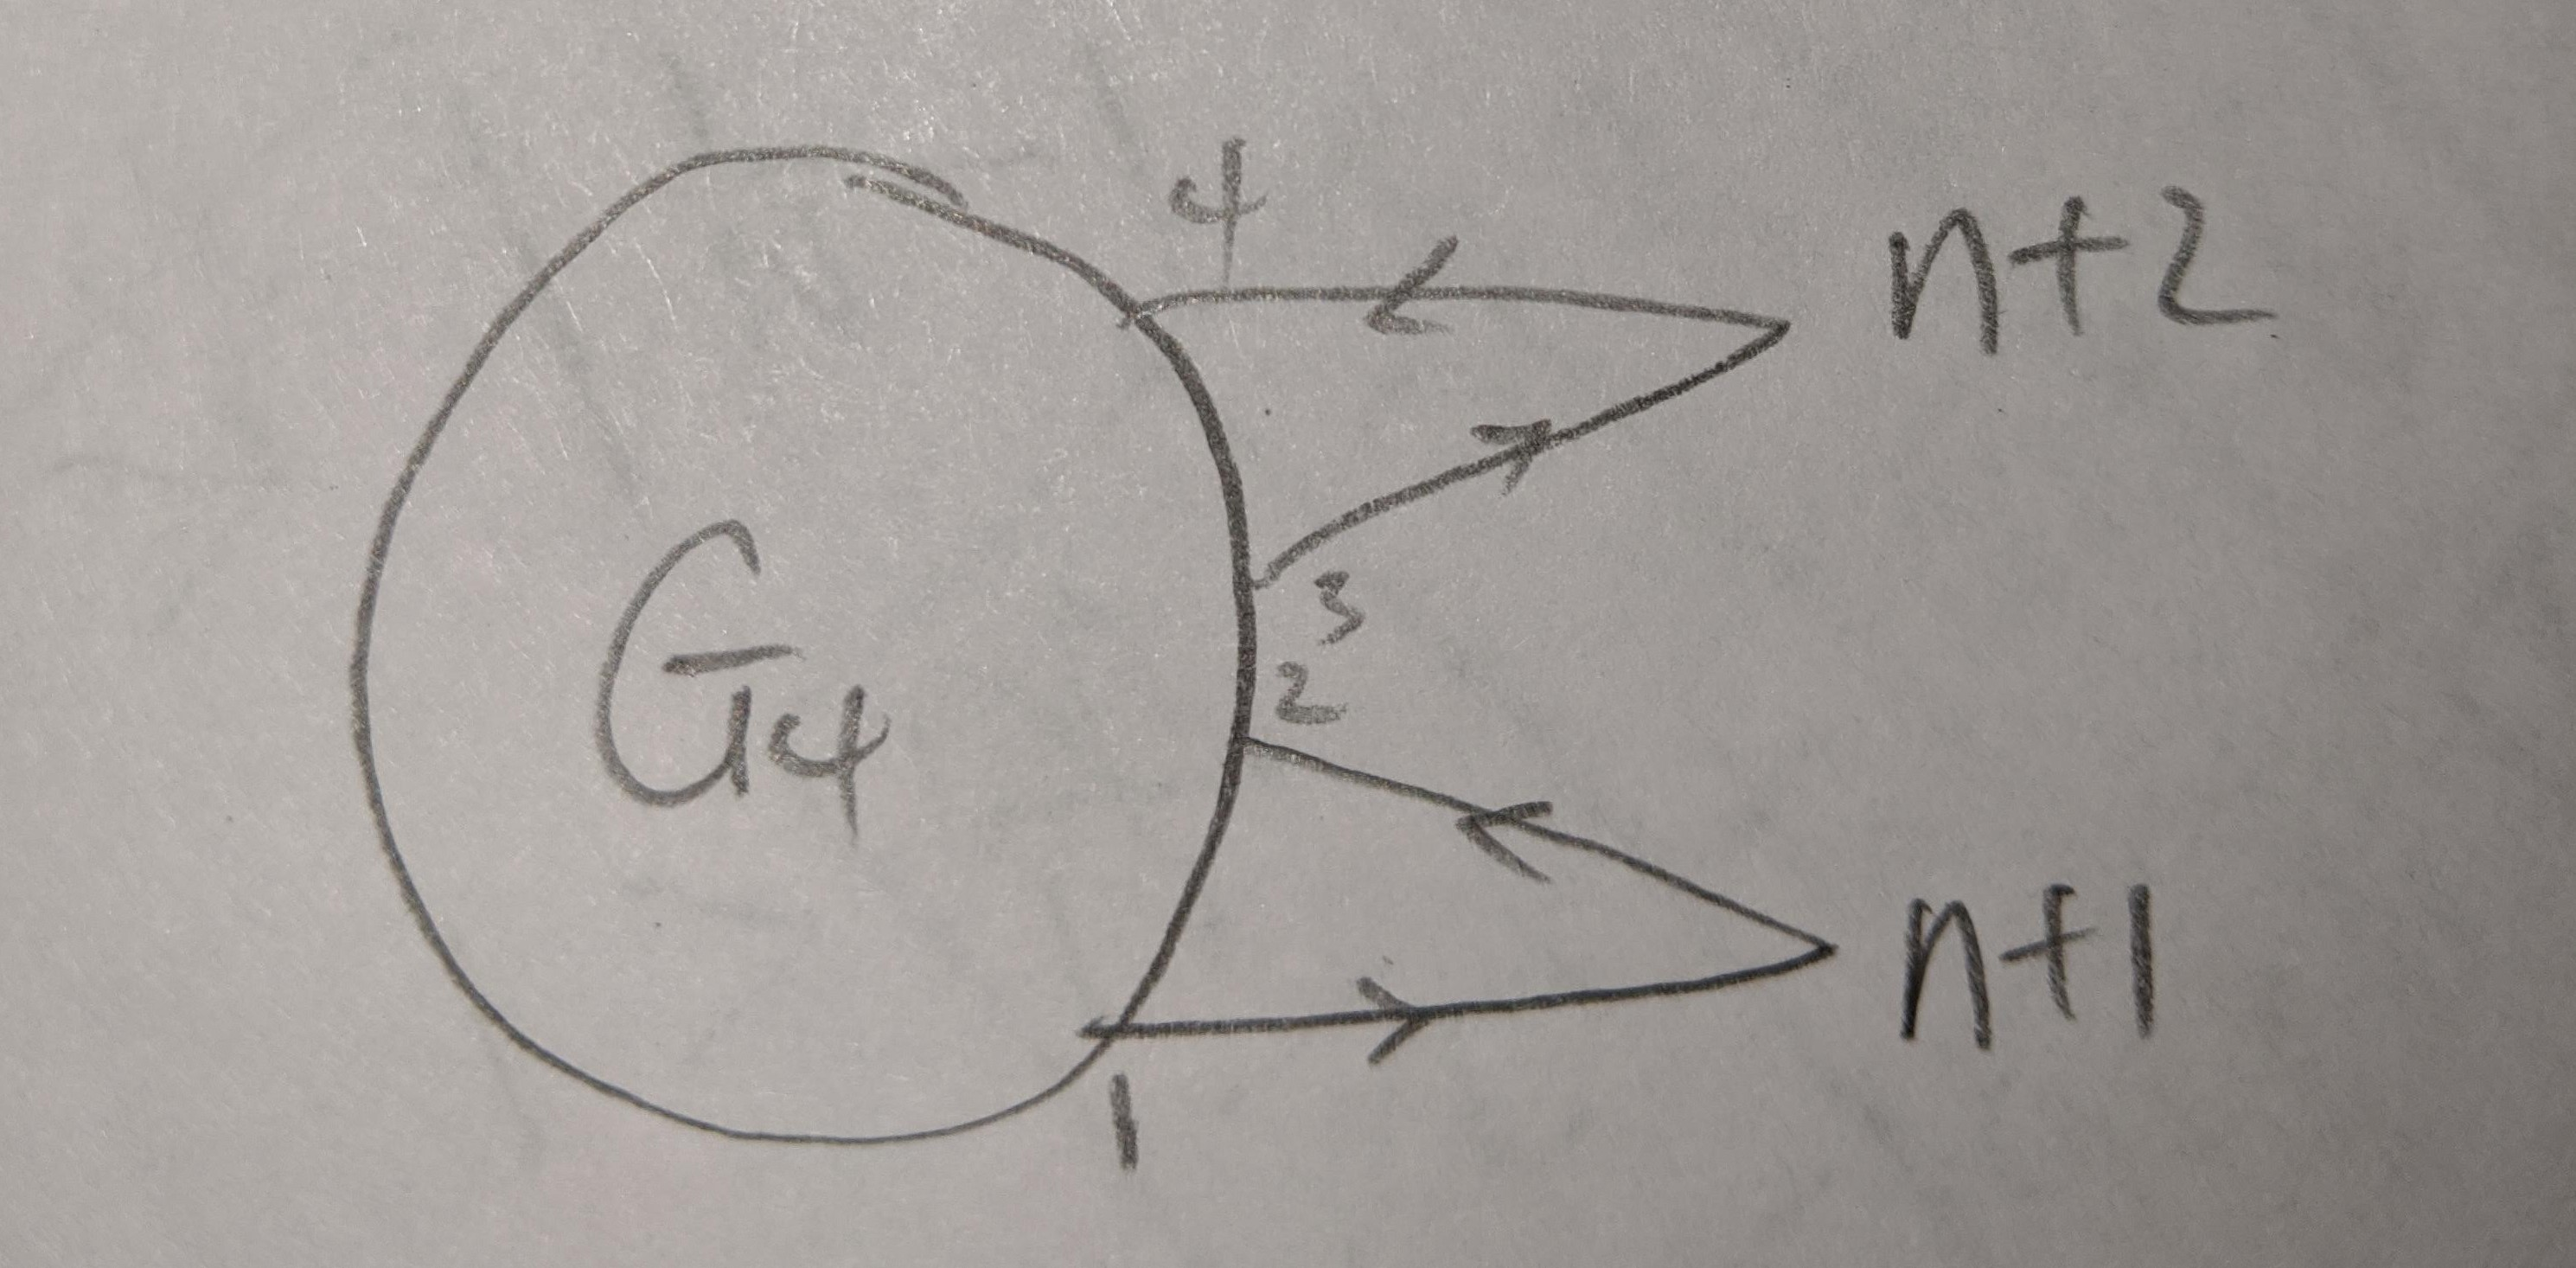
\includegraphics[scale=0.05]{graph2_4.jpg}
\ethm

\bpf
Let $VH_2(G)$ be directed handle graph with 2 handles, and let $T$ be a spanning tree in $VH_2(G)$. Suppose $T$ is rooted at vertex $v_4\in V(G)$. Let the inflow edge to $v_1$ be $e_2$ and the inflow edge to $v_4$ be $e_2$.\\
Case 1. $e_1 \notin T$ and $e_2 \notin T$.\\
Then $\tau(VH_2(G))_4=\tau(G)$ by \Cref{bij_count}.\\
Case 2. $e_2 \in T$.\\
This contradicts with $T$ is rooted at $e_4$.\\
Case 3. $e_1\in T$ and $e_2 \notin T$.\\
By \Cref{symhandle}, there does not exist a path between $v_1$ and $v_2$. Then by \Cref{bij_count}, $\tau(VH_2(G))_4 = \tau_{(1)(2)}(G)$\\
Therefore, the total number of subgraphs of $VH(G)$ is \[
\tau(VH_2(G))_4 = \tau(G) + \tau_{(1)(2)}(G)
\]
\epf

\bthm
{\bf (Rooted at 0)}
Let $VH_2(G)$ be directed handle graph with 2 handles, and let $T$ be a spanning tree in $VH_2(G)$. If $T$ is rooted at vertex $v_0\in V(G)$ as shown in the picture below,
then the total number of subgraphs of $VH_2(G)$ is  
\begin{multline*}
\tau(VH_2(G))_0 = \tau(G) + \tau_{(1)(2)}(G)+ \tau_{(3)(4)}(G)\\ + \tau_{(013)(2)(4)}(G) + \tau_{(01)(23)(4)}(G) + \tau_{(03)(2)(14)}(G)
\end{multline*}
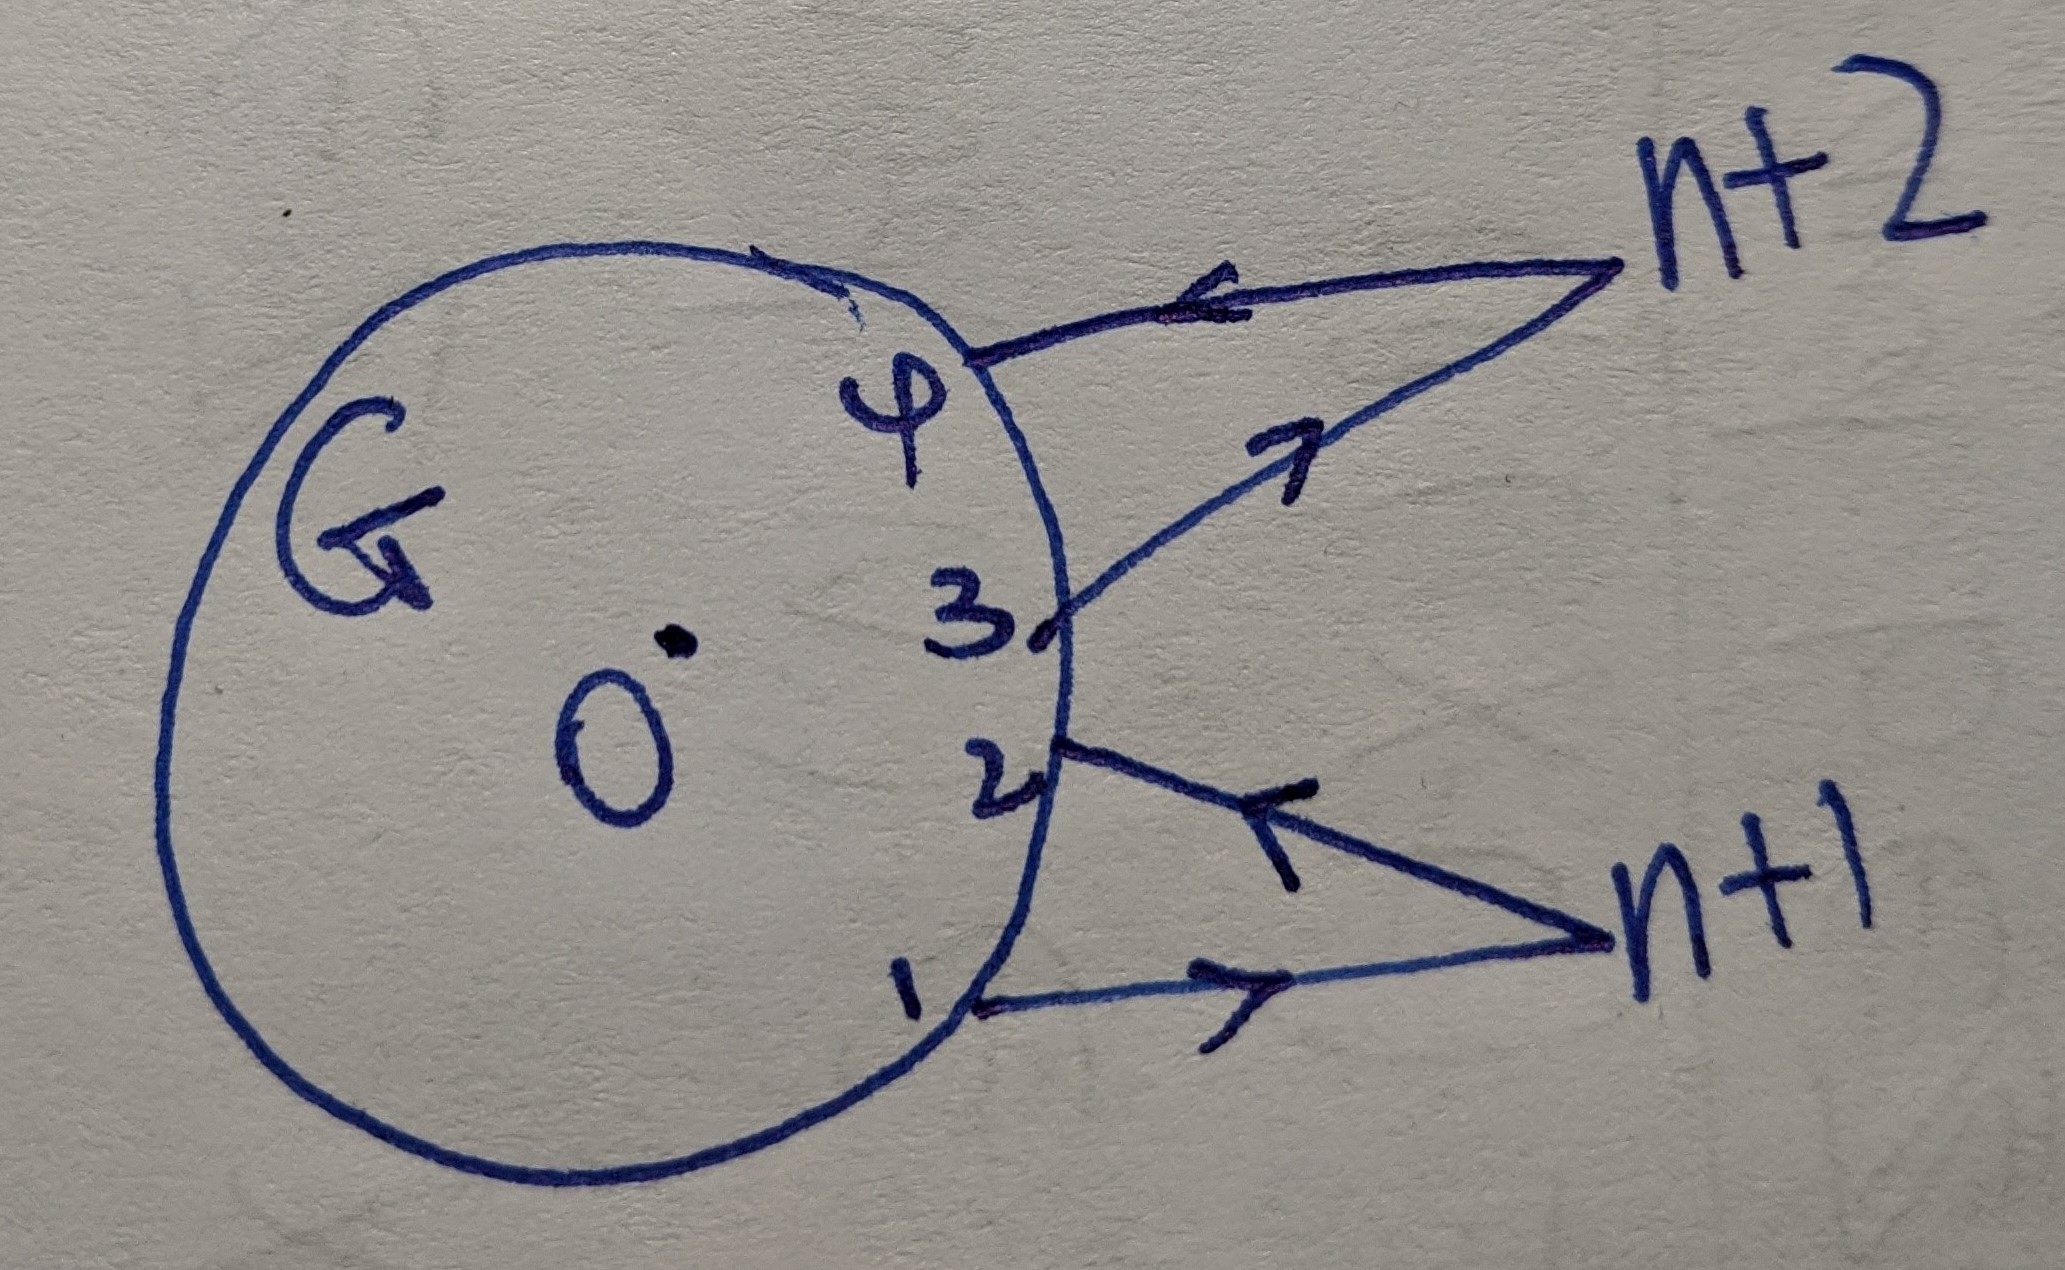
\includegraphics[scale=0.05]{graph2_0.jpg}
\ethm

\bpf
Let $VH_2(G)$ be directed handle graph with 2 handles, and let $T$ be a spanning tree in $VH_2(G)$. Suppose $T$ is rooted at vertex $v_0\in V(G)$. Let the inflow edge to $v_2$ be $e_1$ and the inflow edge to $v_4$ be $e_2$.

Case 1. $e_1 \notin T$ and $e_2 \notin T$.

Then the subgraph rooted at $v_0$ is $\tau(VH_2(G))_0=\tau(G)$ by \Cref{bij_count}.

Case 2. Either $e_1 \in T$ or $e_2 \notin T$

By \Cref{symhandle}, there does not exist a path between $v_1$ and $v_2$ nor between $v_3$ and $v_4$.

So, the subgraph rooted at $v_0$ is $\tau(VH_2(G))_0=\tau_{(1)(2)}(G)+ \tau_{(3)(4)}(G)$ 

Case 4. $e_1\in T$ and $e_2 \in T$.

By \Cref{symhandle}, there does not exist a path between $v_1$ and $v_2$, and there does not exist a path between $v_3$ and $v_4$. So the subgraph rooted at $v_0$ is $\tau_{(013)(2)(4)}(G) + \tau_{(01)(23)(4)}(G) + \tau_{(03)(2)(14)}(G)$

Combining three cases, the total number of subgraphs of $VH(G)$ is \begin{multline*}
\tau(VH_2(G))_0 = \tau(G) + \tau_{(1)(2)}(G)+ \tau_{(3)(4)}(G)\\ + \tau_{(013)(2)(4)}(G) + \tau_{(01)(23)(4)}(G) + \tau_{(03)(2)(14)}(G)
\end{multline*}
\epf

\section{Three Handles.}
\bthm
{\bf (Rooted at 1)}
Let $VH(G)$ be directed handle graph with 3 handles, and let $T$ be a spanning tree in $VH(G)$. If $T$ is rooted at vertex $v_1\in V(G)$ as shown in the picture below,
then the total number of subgraphs of $VH(G)$ is  
\begin{equation*}
    \begin{split}
        \tau(VH_3(G))_1 &= \tau(G) + \tau_{(1)(2)}(G)+ \tau_{(3)(4)}(G) + \tau_{(5)(6)}(G)\\ 
        &+ \tau_{(13)(2)(4)}(G) + \tau_{(1)(23)(4)}(G) + \tau_{(15)(2)(6)}(G) + \tau_{(1)(25)(6)}(G)\\
        &+ \tau_{(135)(4)(6)}(G) + \tau_{(13)(45)(6)}(G) + \tau_{(15)(36)(4)}(G)\\
        &+ \tau_{(135)(2)(4)(6)}(G) + \tau_{(13)(2)(45)(6)}(G) + \tau_{(13)(25)(4)(6)}(G)\\
&+ \tau_{(15)(2)(4)(36)}(G) + \tau_{(15)(23)(4)(6)}(G)
    \end{split}
\end{equation*}
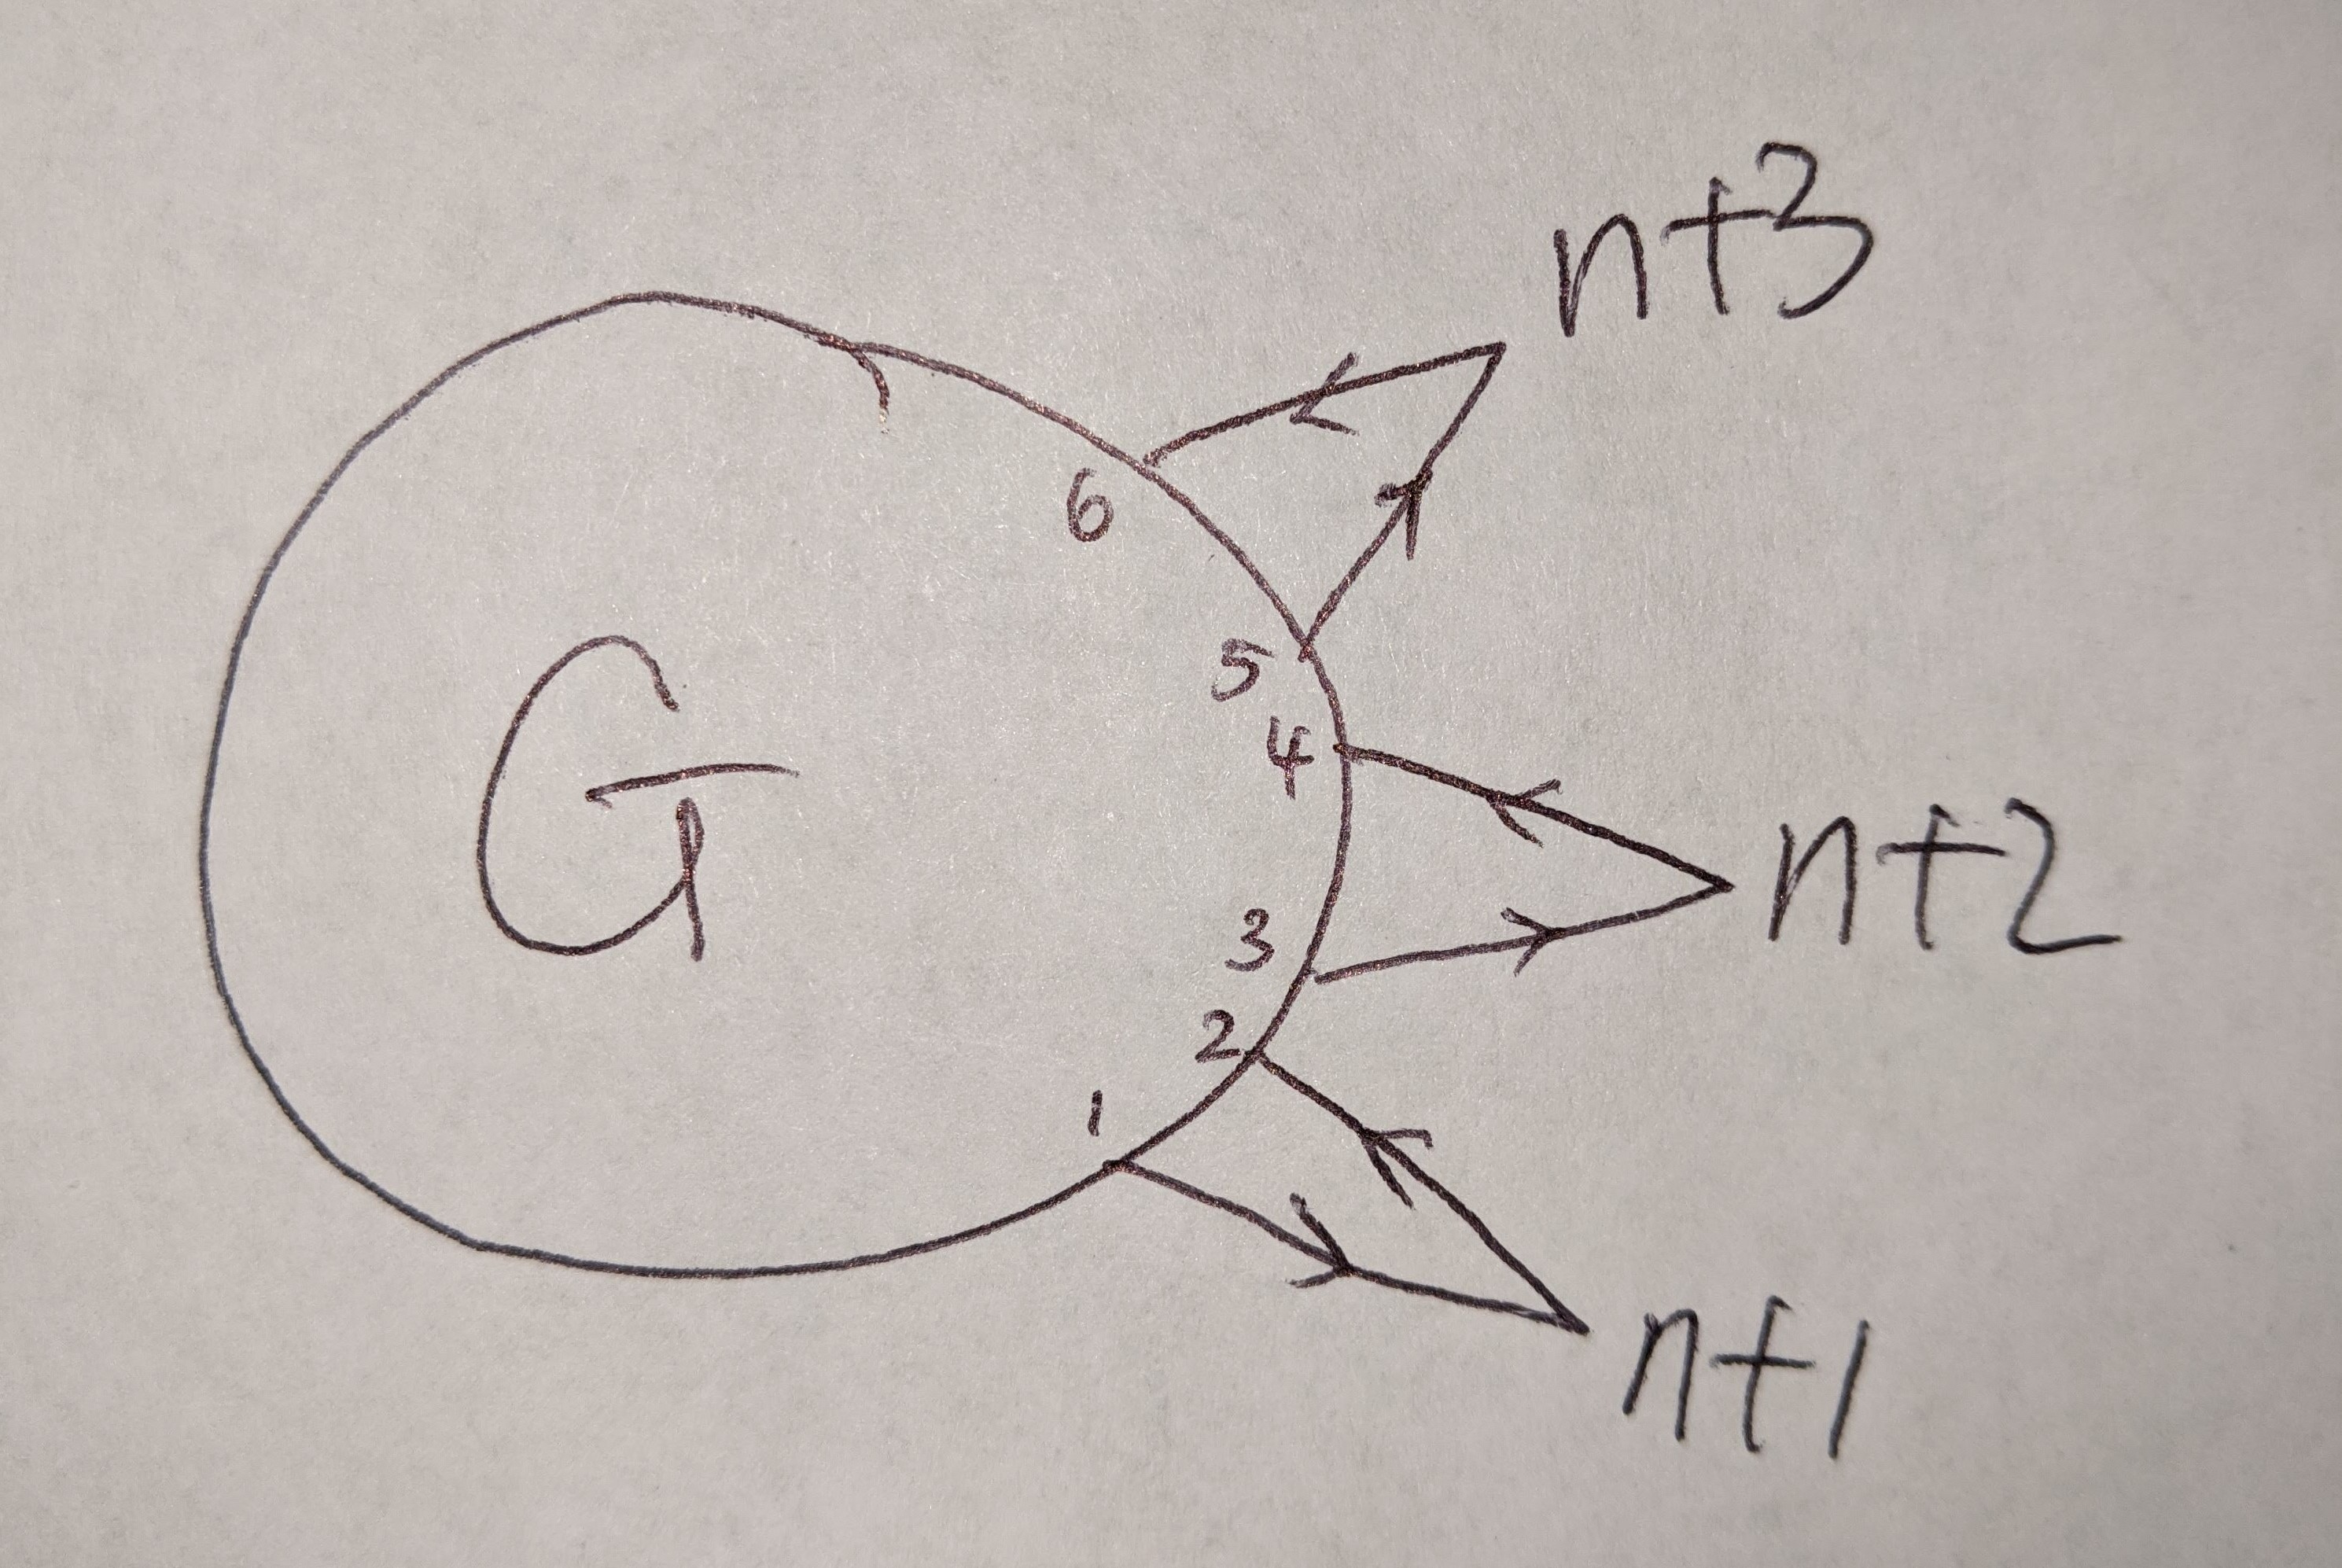
\includegraphics[scale=0.025]{graph3_1.jpg}
\ethm

\bpf
Let $VH(G)$ be directed handle graph with 3 handles, and let $T$ be a spanning tree in $VH(G)$. Suppose $T$ is rooted at vertex $v_1\in V(G)$. Let $e_1$ be the inflow edge to node 2, $e_2$ be the inflow edge to node 4, and $e_3$ be the inflow edge to node 6. Then there are four cases.

Case 1. $e_1\notin VH(G)$, $e_2\notin VH(G)$, and $e_3\notin VH(G)$. Then the number of spanning tree is $\tau(G)$.

Case 2. Only one of $e_1, e_2, e_3$ is in $VH(G)$. 

By \Cref{symhandle}, there does not exist a path between $v_1$ and $v_2$, or between $v_3$ and $v_4$, or between $v_5$ and $v_6$ .

So, the subgraph rooted at node 1 is $\tau_{(1)(2)}(G)+ \tau_{(3)(4)}(G)+ \tau_{(5)(6)}(G)$

Case 3. Two of $e_1, e_2, e_3$ are in $VH(G)$. 
\begin{enumerate}
    \item $e_1\in VH(G)$, $e_2\in VH(G)$, and $e_3\notin VH(G)$.
    
    By \cref{symhandle}, there does not exist path between node 1,2 and node 3,4. Then the number of spanning tree is $\tau_{(13)(2)(4)}(G) + \tau_{(1)(23)(4)}(G)$.
    
    \item $e_1\in VH(G)$, $e_2\notin VH(G)$, and $e_3\in VH(G)$.
    
    By \cref{symhandle}, there does not exist path between node 1,2 and node 5,6. Then the number of spanning tree is $tau_{(15)(2)(6)}(G) + \tau_{(1)(25)(6)}(G)$.
    
    \item $e_1\notin VH(G)$, $e_2\in VH(G)$, and $e_3\in VH(G)$.
    
    By \cref{symhandle}, there does not exist path between node 3,4 and node 5,6. Then the number of spanning tree is $\tau_{(135)(4)(6)}(G) + \tau_{(13)(45)(6)}(G) + \tau_{(15)(36)(4)}(G)$.
\end{enumerate}

Case 4. All of $e_1, e_2, e_3$ are in $VH(G)$. 

By \cref{symhandle}, there does not exist path between node 1,2 and node 3,4 and node 5,6. Then the number of spanning tree is $$\tau_{(135)(2)(4)(6)}(G) + \tau_{(13)(2)(45)(6)}(G) + \tau_{(13)(25)(4)(6)}(G)\\
&+ \tau_{(15)(2)(4)(36)}(G) + \tau_{(15)(23)(4)(6)}(G)$$

Therefore, the total number of subgraphs of $VH(G)$ is  
\begin{equation*}
    \begin{split}
        \tau(VH_3(G))_1 &= \tau(G) + \tau_{(1)(2)}(G)+ \tau_{(3)(4)}(G) + \tau_{(5)(6)}(G)\\ 
        &+ \tau_{(13)(2)(4)}(G) + \tau_{(1)(23)(4)}(G) + \tau_{(15)(2)(6)}(G) + \tau_{(1)(25)(6)}(G)\\
        &+ \tau_{(135)(4)(6)}(G) + \tau_{(13)(45)(6)}(G) + \tau_{(15)(36)(4)}(G)\\
        &+ \tau_{(135)(2)(4)(6)}(G) + \tau_{(13)(2)(45)(6)}(G) + \tau_{(13)(25)(4)(6)}(G)\\
&+ \tau_{(15)(2)(4)(36)}(G) + \tau_{(15)(23)(4)(6)}(G)
    \end{split}
\end{equation*}
\epf

\bthm
{\bf (Rooted at 2)}
Let $VH(G)$ be directed handle graph with 3 handles, and let $T$ be a spanning tree in $VH(G)$. If $T$ is rooted at vertex $v_2\in V(G)$ as shown in the picture below,
then the total number of subgraphs of $VH(G)$ is  
\[
\tau(VH_3(G))_2 = \tau(G) + \tau_{(3)(4)}(G) + \tau_{(5)(6)}(G) + \tau_{(3)(45)(6)}(G)+ \tau_{(35)(4)(6)}(G)
\]
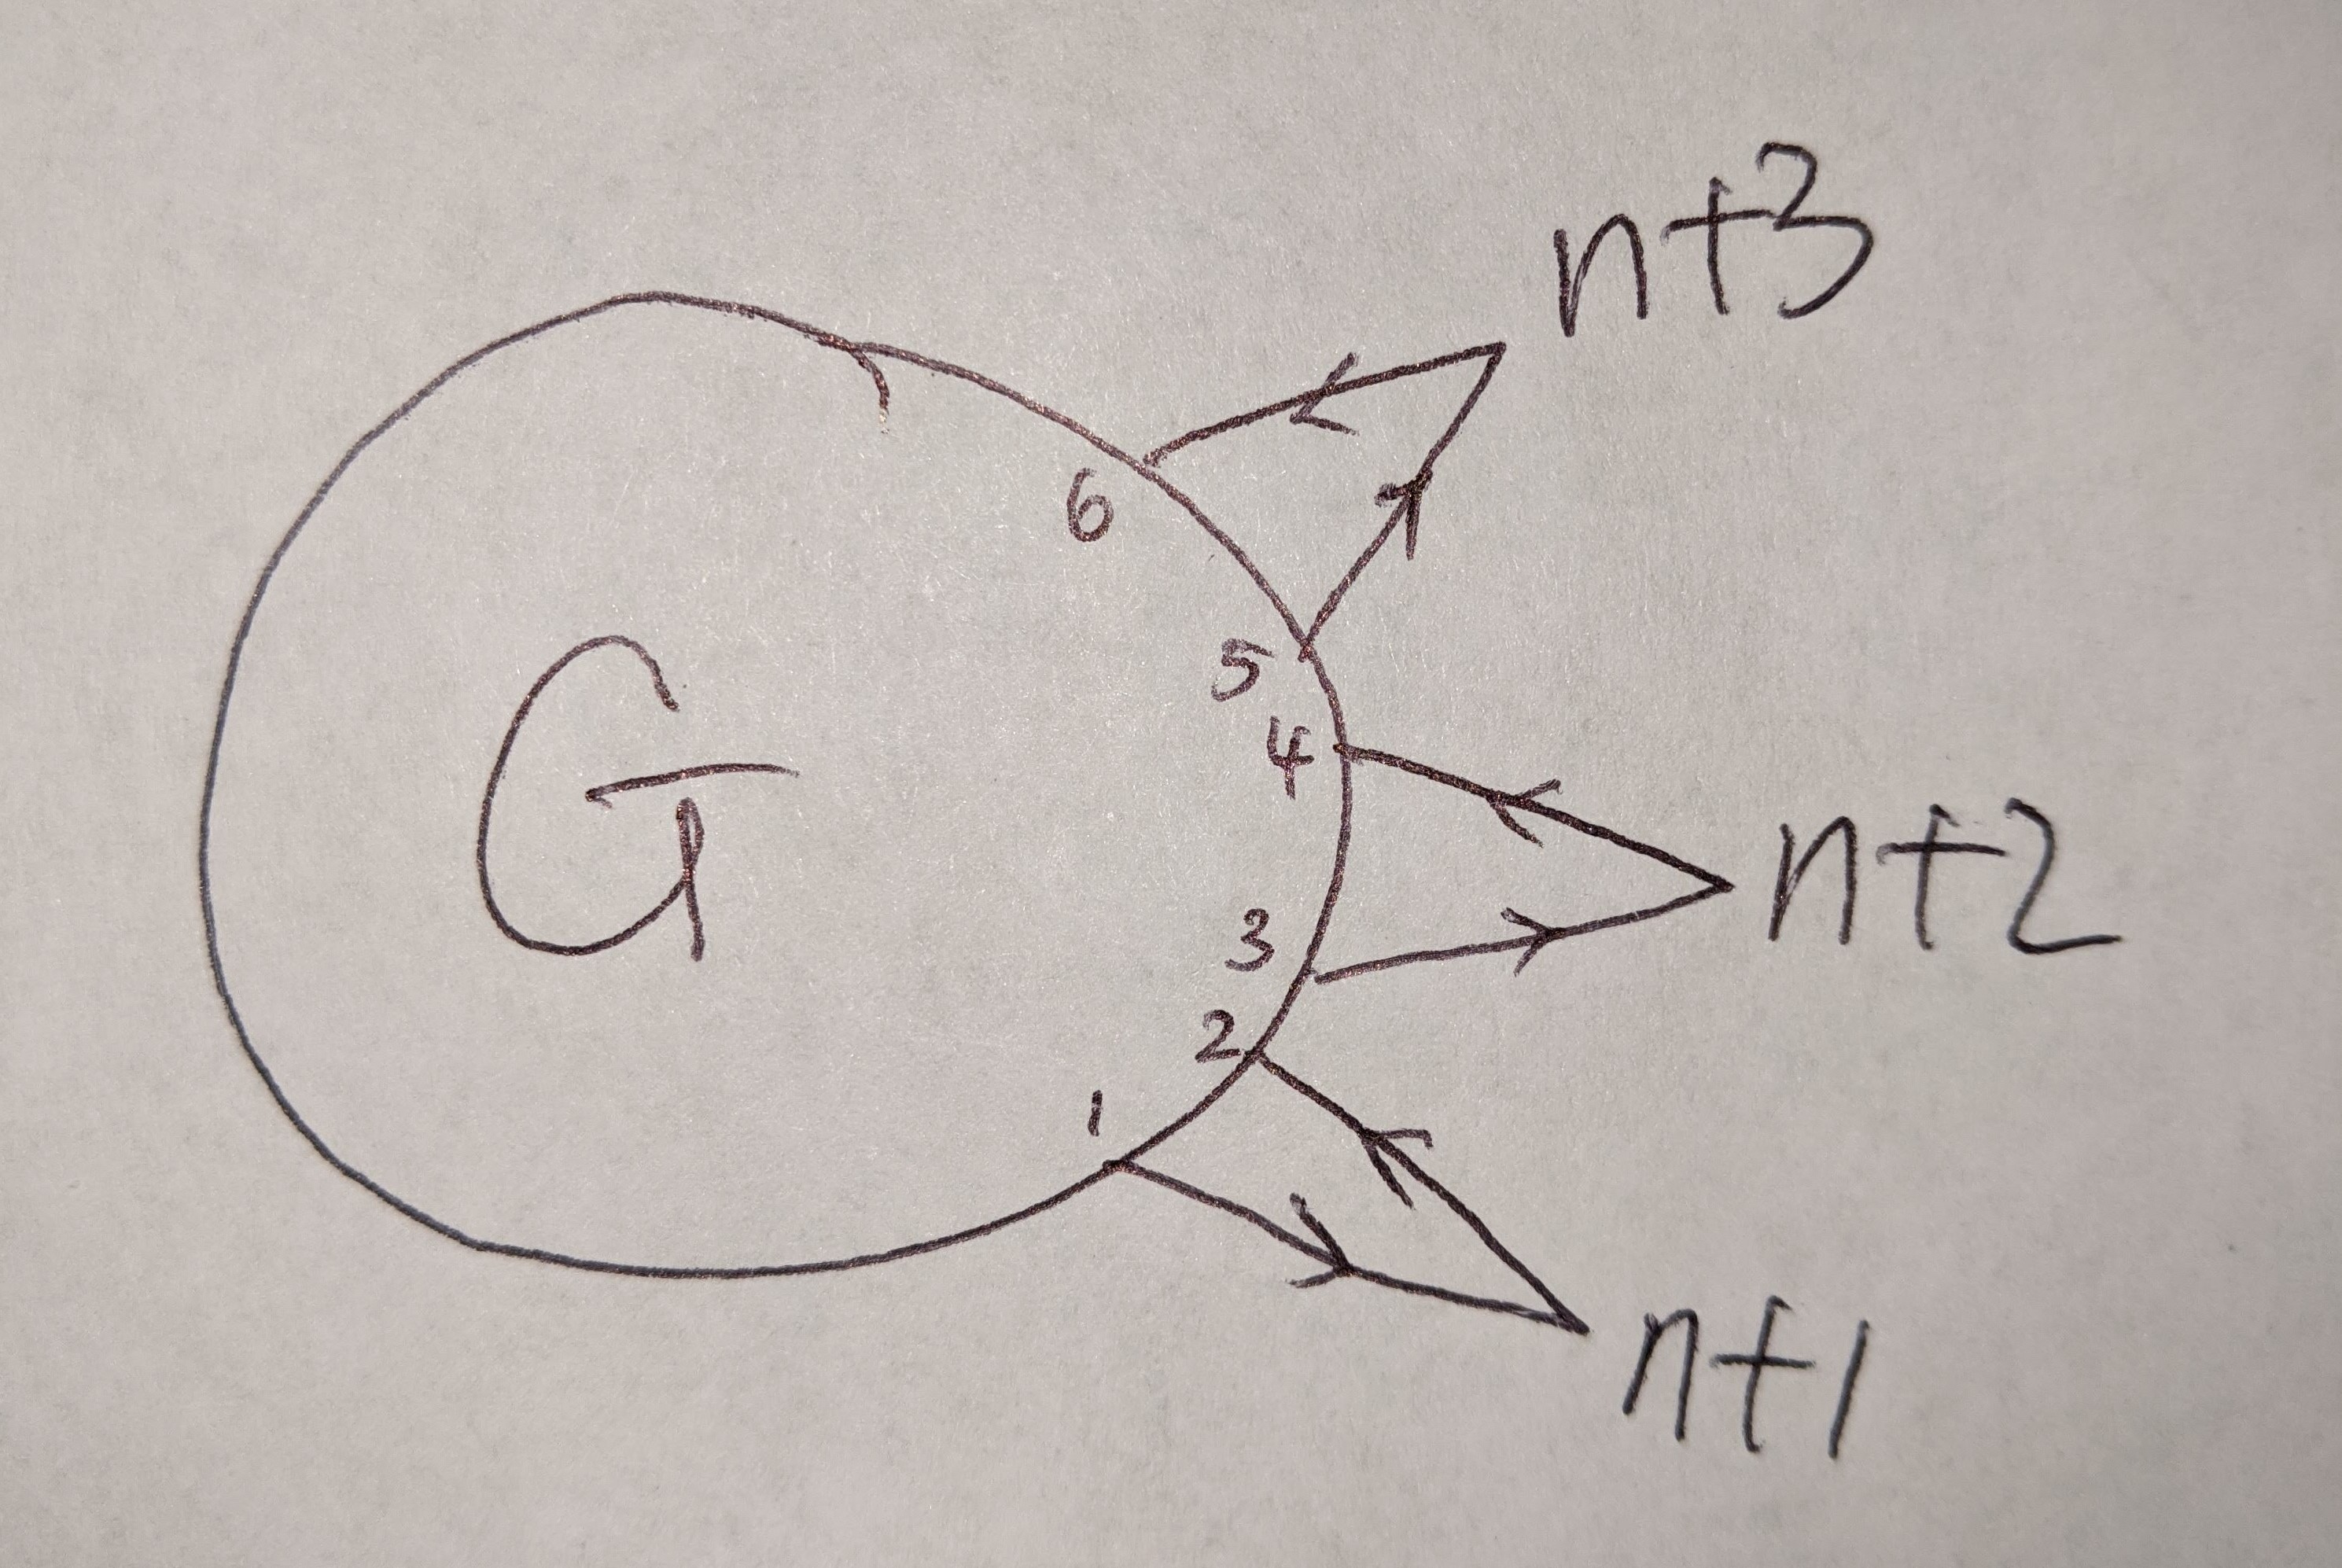
\includegraphics[scale=0.025]{graph3_1.jpg}
\ethm

\bpf
Let $VH(G)$ be directed handle graph with 3 handles, and let $T$ be a spanning tree in $VH(G)$. Suppose $T$ is rooted at vertex $v_2\in V(G)$. Let $e_1$ be the inflow edge to node 2, $e_2$ be the inflow edge to node 4, and $e_3$ be the inflow edge to node 6. Since $T$ is rooted at 2, $e_1 \notin VH(G)$. Therefore, there are three cases.

Case 1. Case 1. $e_2\notin VH(G)$, and $e_3\notin VH(G)$. Then the number of spanning tree is $\tau(G)$.

Case 2. Only one of $e_2, e_3$ is in $VH(G)$. 

By \Cref{symhandle}, there does not exist a path between $v_3$ and $v_4$ or between $v_5$ and $v_6$.

So, the subgraph rooted at node 2 is $\tau_{(3)(4)}(G)+ \tau_{(5)(6)}(G)$

Case 3. Both of $e_2, e_3$ are in $VH(G)$.

By \cref{symhandle}, there does not exist path between node 3,4 and 5,6. Then the number of spanning tree is $\tau_{(3)(45)(6)}(G)+ \tau_{(35)(4)(6)}(G)$.

Therefore, the total number of subgraphs of $VH(G)$ is  \[
\tau(VH_3(G))_2 = \tau(G) + \tau_{(3)(4)}(G) + \tau_{(5)(6)}(G) + \tau_{(3)(45)(6)}(G)+ \tau_{(35)(4)(6)}(G)
\]
\epf

\bthm
{\bf (Rooted at 3)}
Let $VH(G)$ be directed handle graph with 3 handles, and let $T$ be a spanning tree in $VH(G)$. If $T$ is rooted at vertex $v_3\in V(G)$ as shown in the picture below,
then the total number of subgraphs of $VH(G)$ is  
\begin{equation*}
    \begin{split}
        \tau(VH_3(G))_3 &= \tau(G) + \tau_{(1)(2)}(G)+ \tau_{(3)(4)}(G) + \tau_{(5)(6)}(G)\\ 
        &+ \tau_{(35)(4)(6)}(G) + \tau_{(3)(45)(6)}(G) + \tau_{(13)(2)(4)}(G) + \tau_{(3)(14)(2)}(G)\\
        &+ \tau_{(135)(2)(6)}(G) + \tau_{(35)(16)(2)}(G) + \tau_{(13)(25)(6)}(G)\\
        &+ \tau_{(135)(2)(4)(6)}(G) + \tau_{(35)(16)(2)(4)}(G) + \tau_{(35)(14)(2)(6)}(G)\\
&+ \tau_{(13)(25)(6)(4)}(G) + \tau_{(13)(45)(2)(6)}(G)
    \end{split}
\end{equation*}
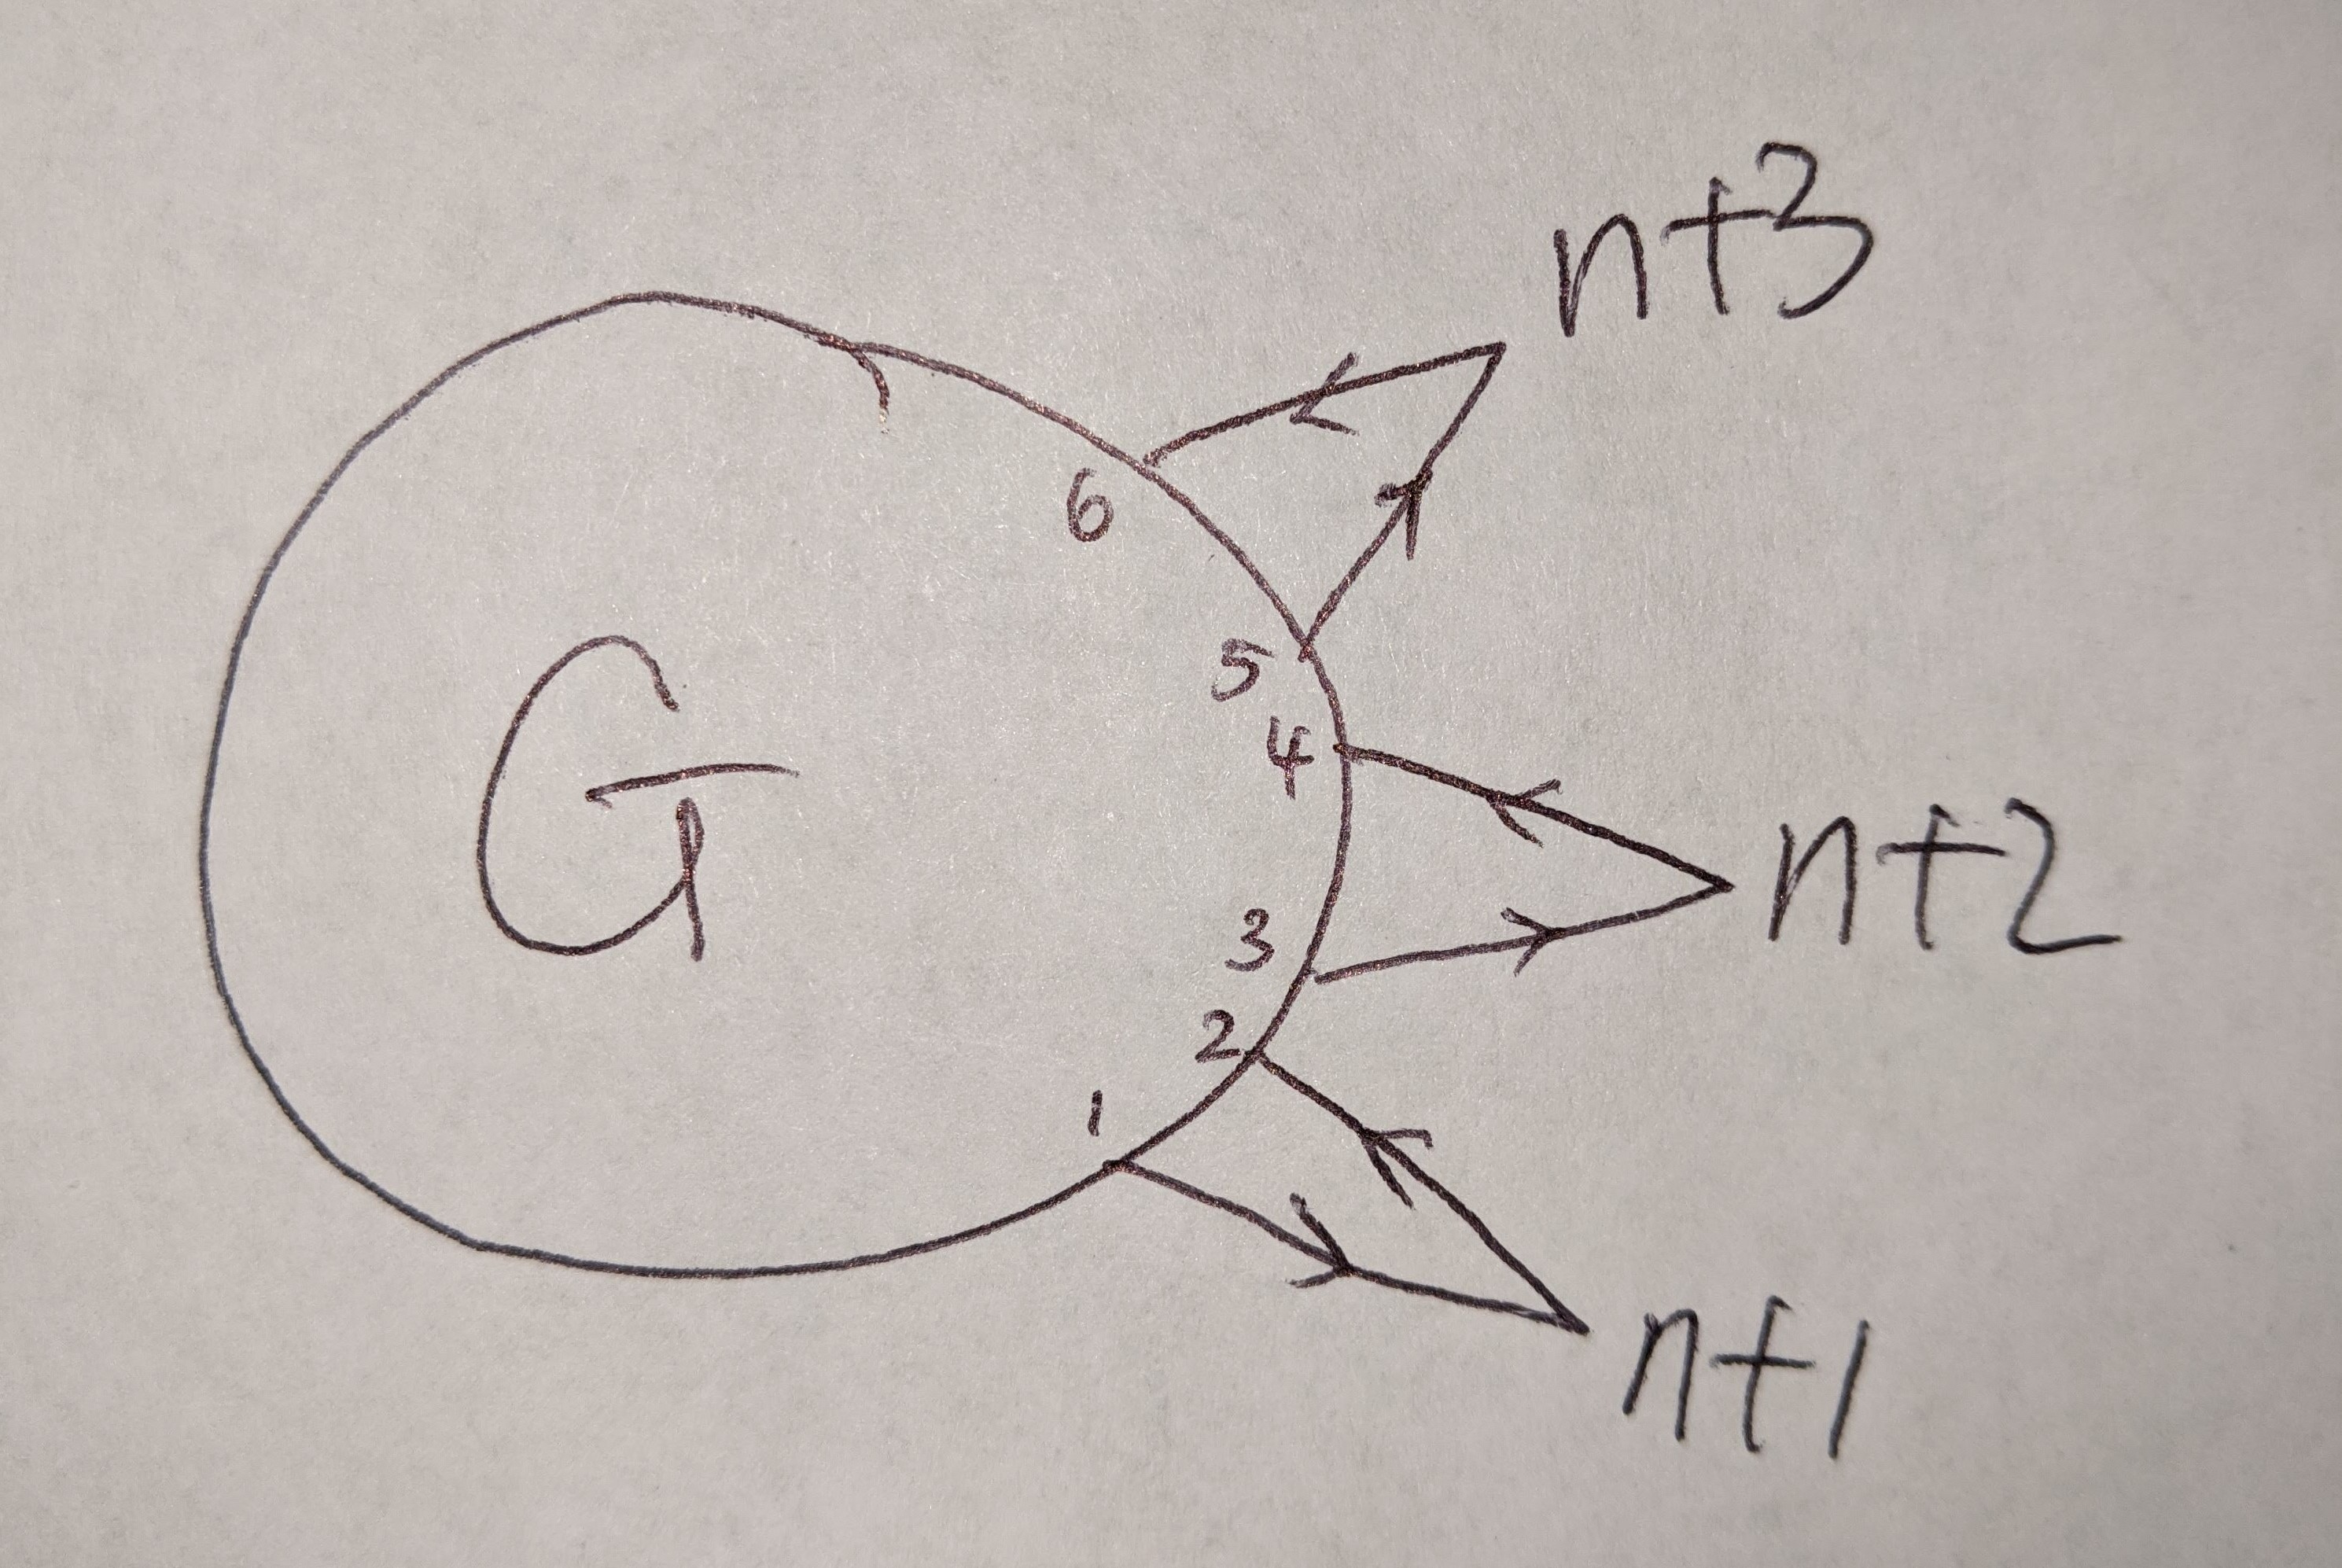
\includegraphics[scale=0.025]{graph3_1.jpg}
\ethm

\bpf
Let $VH(G)$ be directed handle graph with 3 handles, and let $T$ be a spanning tree in $VH(G)$. Suppose $T$ is rooted at vertex $v_3\in V(G)$. Let $e_1$ be the inflow edge to node 2, $e_2$ be the inflow edge to node 4, and $e_3$ be the inflow edge to node 6. Then there are four cases.

Case 1. $e_1\notin VH(G)$, $e_2\notin VH(G)$, and $e_3\notin VH(G)$. Then the number of spanning tree is $T(G)$.

Case 2. Only one of $e_1, e_2, e_3$ is in $VH(G)$. 

By \Cref{symhandle}, there does not exist a path between $v_1$ and $v_2$, or between $v_3$ and $v_4$, or between $v_5$ and $v_6$ .

So, the subgraph rooted at node 1 is $\tau_{(1)(2)}(G)+ \tau_{(3)(4)}(G)+ \tau_{(5)(6)}(G)$

Case 3. Two of $e_1, e_2, e_3$ are in $VH(G)$. 
\begin{enumerate}
    \item $e_1\in VH(G)$, $e_2\in VH(G)$, and $e_3\notin VH(G)$.
    
    By \cref{symhandle}, there does not exist path between node 1,2 and node 3,4. Then the number of spanning tree is $\tau_{(13)(2)(4)}(G) + \tau_{(3)(14)(2)}(G)$.
    
    \item $e_1\in VH(G)$, $e_2\notin VH(G)$, and $e_3\in VH(G)$.
    
    By \cref{symhandle}, there does not exist path between node 1,2 and node 5,6. Then the number of spanning tree is $\tau_{(135)(2)(6)}(G) + \tau_{(35)(16)(2)}(G) + \tau_{(13)(25)(6)}(G)$.
    
    \item $e_1\notin VH(G)$, $e_2\in VH(G)$, and $e_3\in VH(G)$.
    
    By \cref{symhandle}, there does not exist path between node 3,4 and node 5,6. Then the number of spanning tree is $\tau_{(35)(4)(6)}(G) + \tau_{(3)(45)(6)}(G)$.
\end{enumerate}

Case 4. All of $e_1, e_2, e_3$ are in $VH(G)$. 

By \cref{symhandle}, there does not exist path between node 1,2 and node 3,4 and node 5,6. Then the number of spanning tree is\[
\tau_{(135)(2)(4)(6)}(G) + \tau_{(35)(16)(2)(4)}(G) + \tau_{(35)(14)(2)(6)}(G) \tau_{(13)(25)(6)(4)}(G) + \tau_{(13)(45)(2)(6)}(G)
\]

Therefore, the total number of subgraphs of $VH(G)$ is  
\begin{equation*}
    \begin{split}
        \tau(VH_3(G))_3 &= \tau(G) + \tau_{(1)(2)}(G)+ \tau_{(3)(4)}(G) + \tau_{(5)(6)}(G)\\ 
        &+ \tau_{(35)(4)(6)}(G) + \tau_{(3)(45)(6)}(G) + \tau_{(13)(2)(4)}(G) + \tau_{(3)(14)(2)}(G)\\
        &+ \tau_{(135)(2)(6)}(G) + \tau_{(35)(16)(2)}(G) + \tau_{(13)(25)(6)}(G)\\
        &+ \tau_{(135)(2)(4)(6)}(G) + \tau_{(35)(16)(2)(4)}(G) + \tau_{(35)(14)(2)(6)}(G)\\
&+ \tau_{(13)(25)(6)(4)}(G) + \tau_{(13)(45)(2)(6)}(G)
    \end{split}
\end{equation*}
\epf

\bthm
{\bf (Rooted at 4)}
Let $VH(G)$ be directed handle graph with 3 handles, and let $T$ be a spanning tree in $VH(G)$. If $T$ is rooted at vertex $v_4\in V(G)$ as shown in the picture below,
then the total number of subgraphs of $VH(G)$ is  
\[
\tau(VH_3(G))_4 = \tau(G) + \tau_{(1)(2)}(G)+ \tau_{(5)(6)}(G) + \tau_{(1)(25)(6)}(G)+ \tau_{(15)(2)(6)}(G)
\]
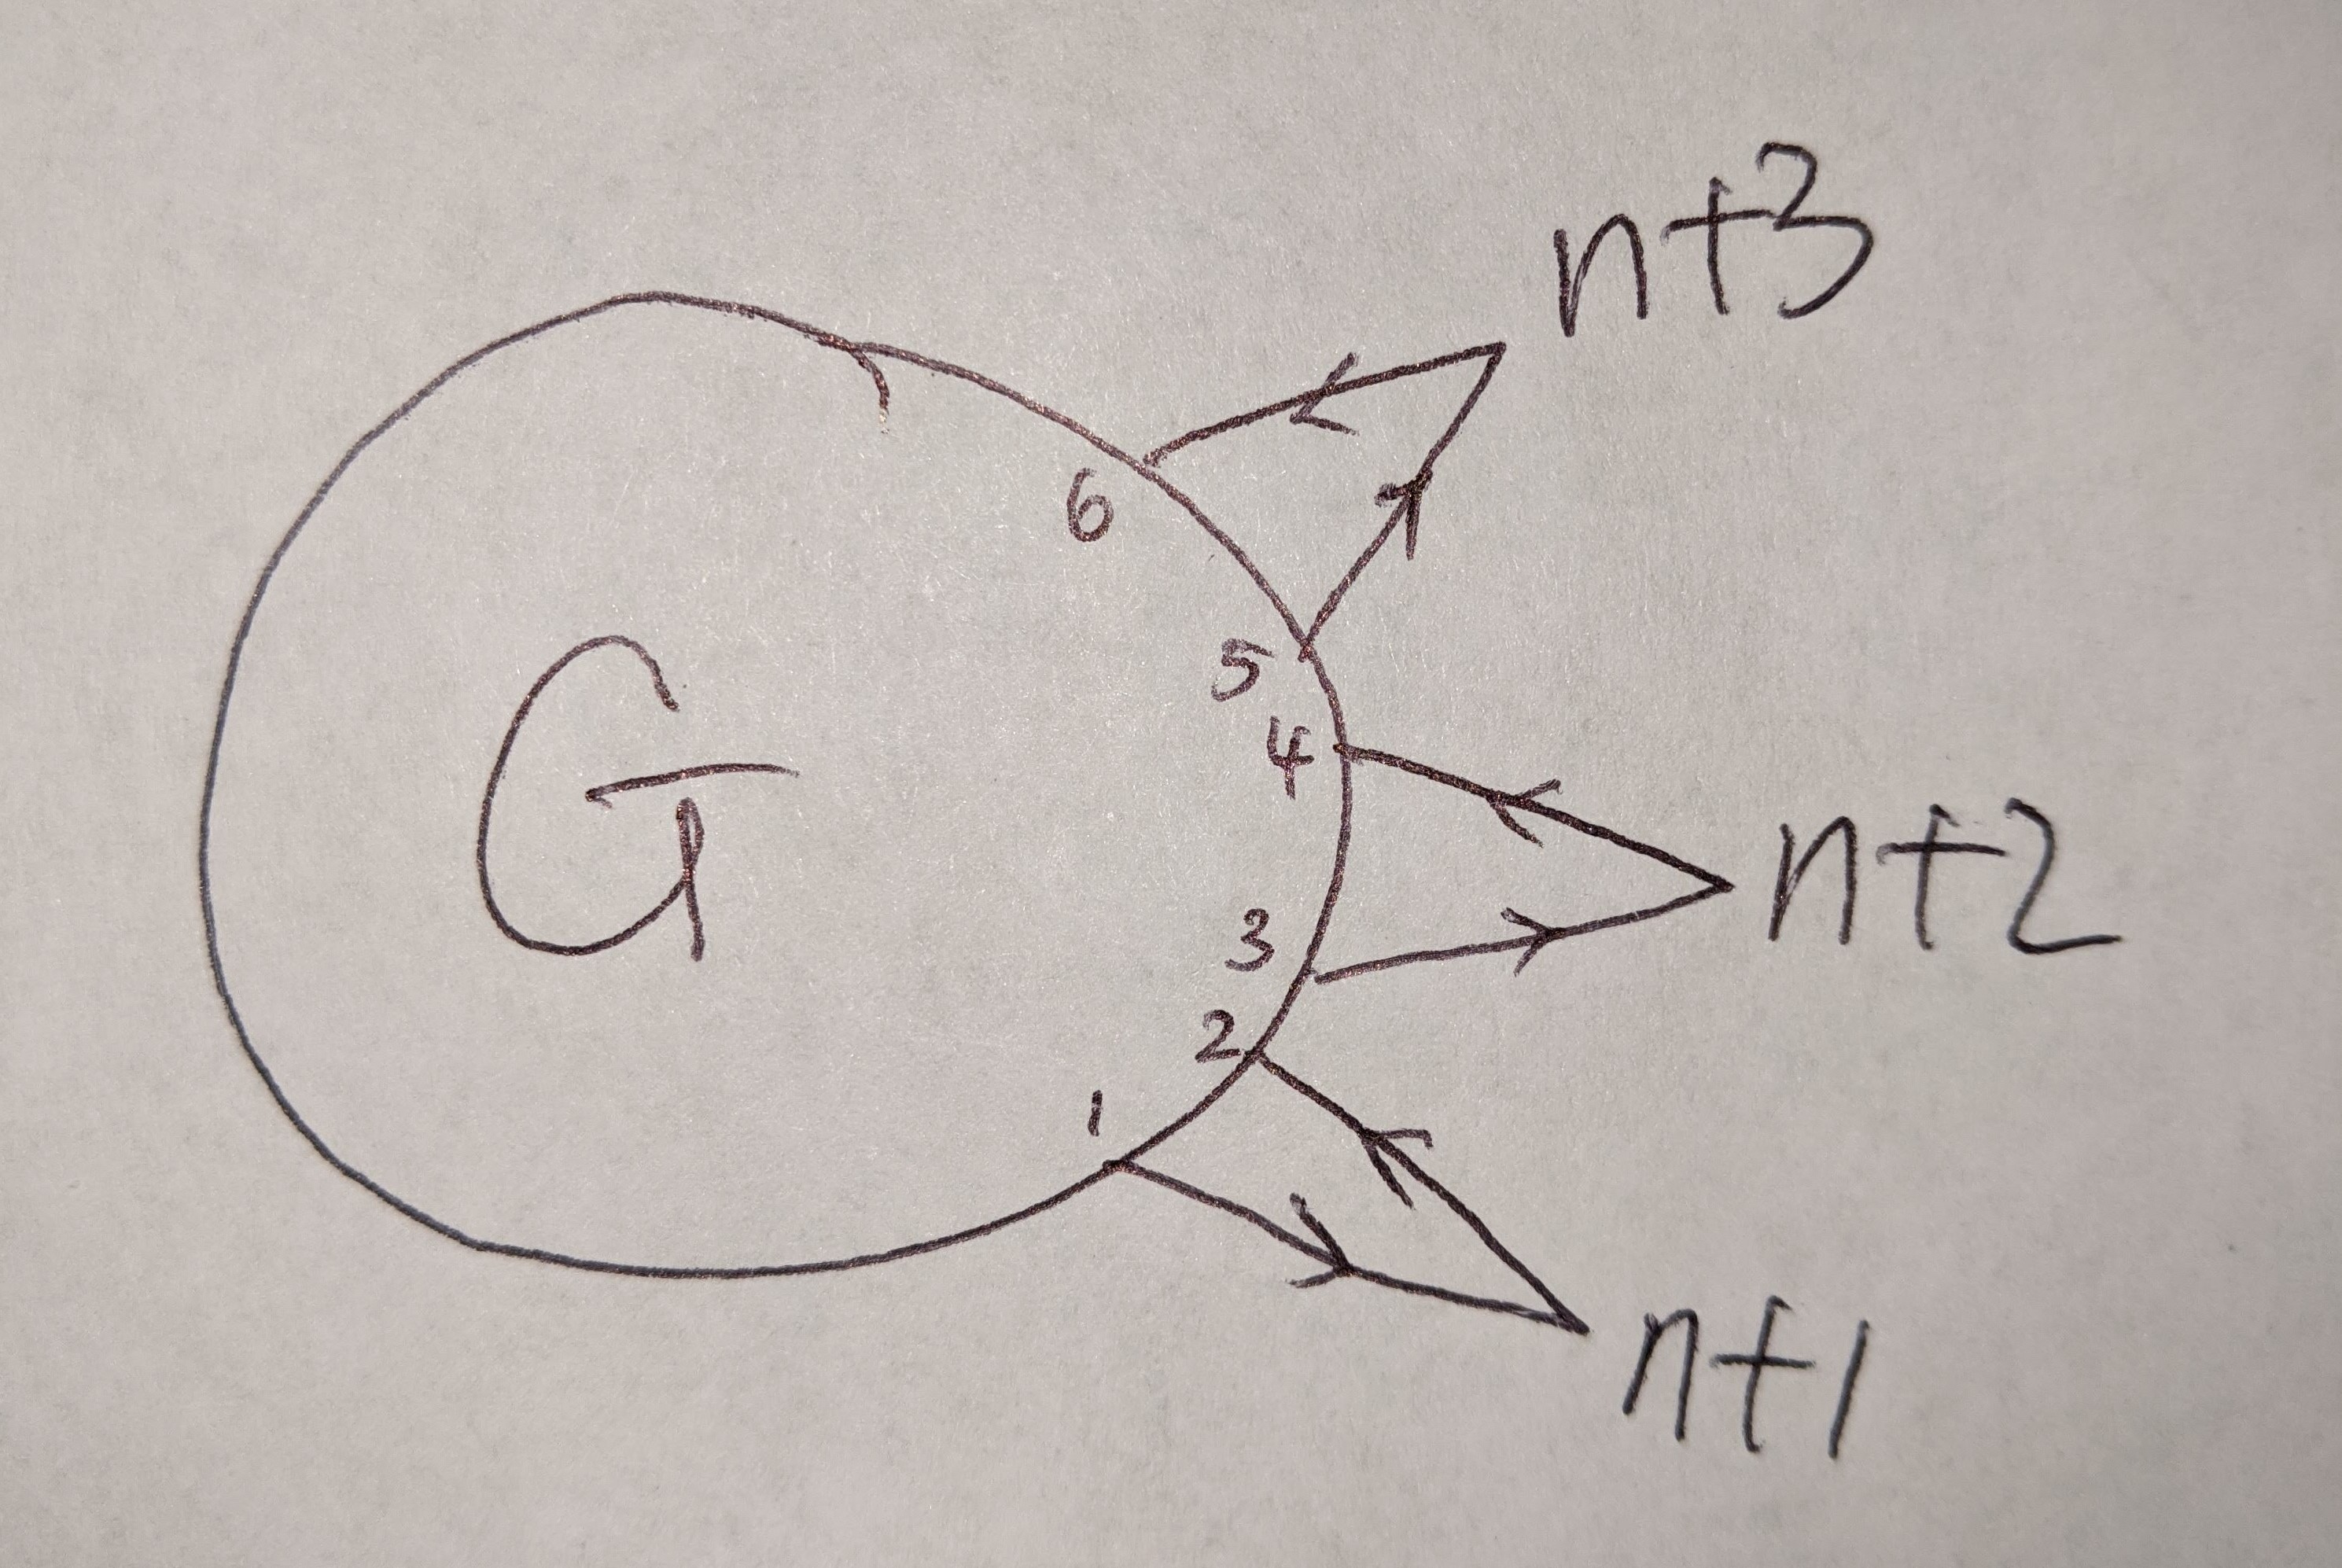
\includegraphics[scale=0.025]{graph3_1.jpg}
\ethm

\bpf
Let $VH(G)$ be directed handle graph with 3 handles, and let $T$ be a spanning tree in $VH(G)$. Suppose $T$ is rooted at vertex $v_4\in V(G)$. Let $e_1$ be the inflow edge to node 2, $e_2$ be the inflow edge to node 4, and $e_3$ be the inflow edge to node 6. Since $T$ is rooted at 4, $e_2 \notin VH(G)$. Therefore, there are three cases.

Case 1. Case 1. $e_1\notin VH(G)$, and $e_3\notin VH(G)$. Then the number of spanning tree is $\tau(G)$.

Case 2. Only one of $e_1, e_3$ is in $VH(G)$. 

By \Cref{symhandle}, there does not exist a path between $v_1$ and $v_2$ or between $v_5$ and $v_6$.

So, the subgraph rooted at node 2 is $\tau_{(1)(2)}(G)+ \tau_{(5)(6)}(G)$

Case 3. Both of $e_2, e_3$ are in $VH(G)$.

By \cref{symhandle}, there does not exist path between node 3,4 and 5,6. Then the number of spanning tree is $\tau_{(1)(25)(6)}(G)+ \tau_{(15)(2)(6)}(G)$.

Therefore, the total number of subgraphs of $VH(G)$ is  \[
\tau(VH_3(G))_4 = \tau(G) + \tau_{(1)(2)}(G)+ \tau_{(5)(6)}(G) + \tau_{(1)(25)(6)}(G)+ \tau_{(15)(2)(6)}(G)
\]
\epf

\bthm
{\bf (Rooted at 5)}
Let $VH(G)$ be directed handle graph with 3 handles, and let $T$ be a spanning tree in $VH(G)$. If $T$ is rooted at vertex $v_5\in V(G)$ as shown in the picture below,
then the total number of subgraphs of $VH(G)$ is  
\begin{equation*}
    \begin{split}
        \tau(VH_3(G))_5 &= \tau(G) + \tau_{(1)(2)}(G)+ \tau_{(3)(4)}(G) + \tau_{(5)(6)}(G)\\ 
        &+ \tau_{(53)(4)(6)}(G) + \tau_{(5)(36)(4)}(G) + \tau_{(15)(2)(6)}(G) + \tau_{(5)(16)(2)}(G)\\
        &+ \tau_{(135)(2)(4)}(G) + \tau_{(15)(23)(4)}(G) + \tau_{(35)(14)(2)}(G)\\
        &+ \tau_{(135)(2)(4)(6)}(G) + \tau_{(15)(23)(4)(6)}(G) + \tau_{(15)(36)(2)(4)}(G)\\
&+ \tau_{(35)(14)(2)(6)}(G) + \tau_{(35)(16)(2)(4)}(G)
    \end{split}
\end{equation*}
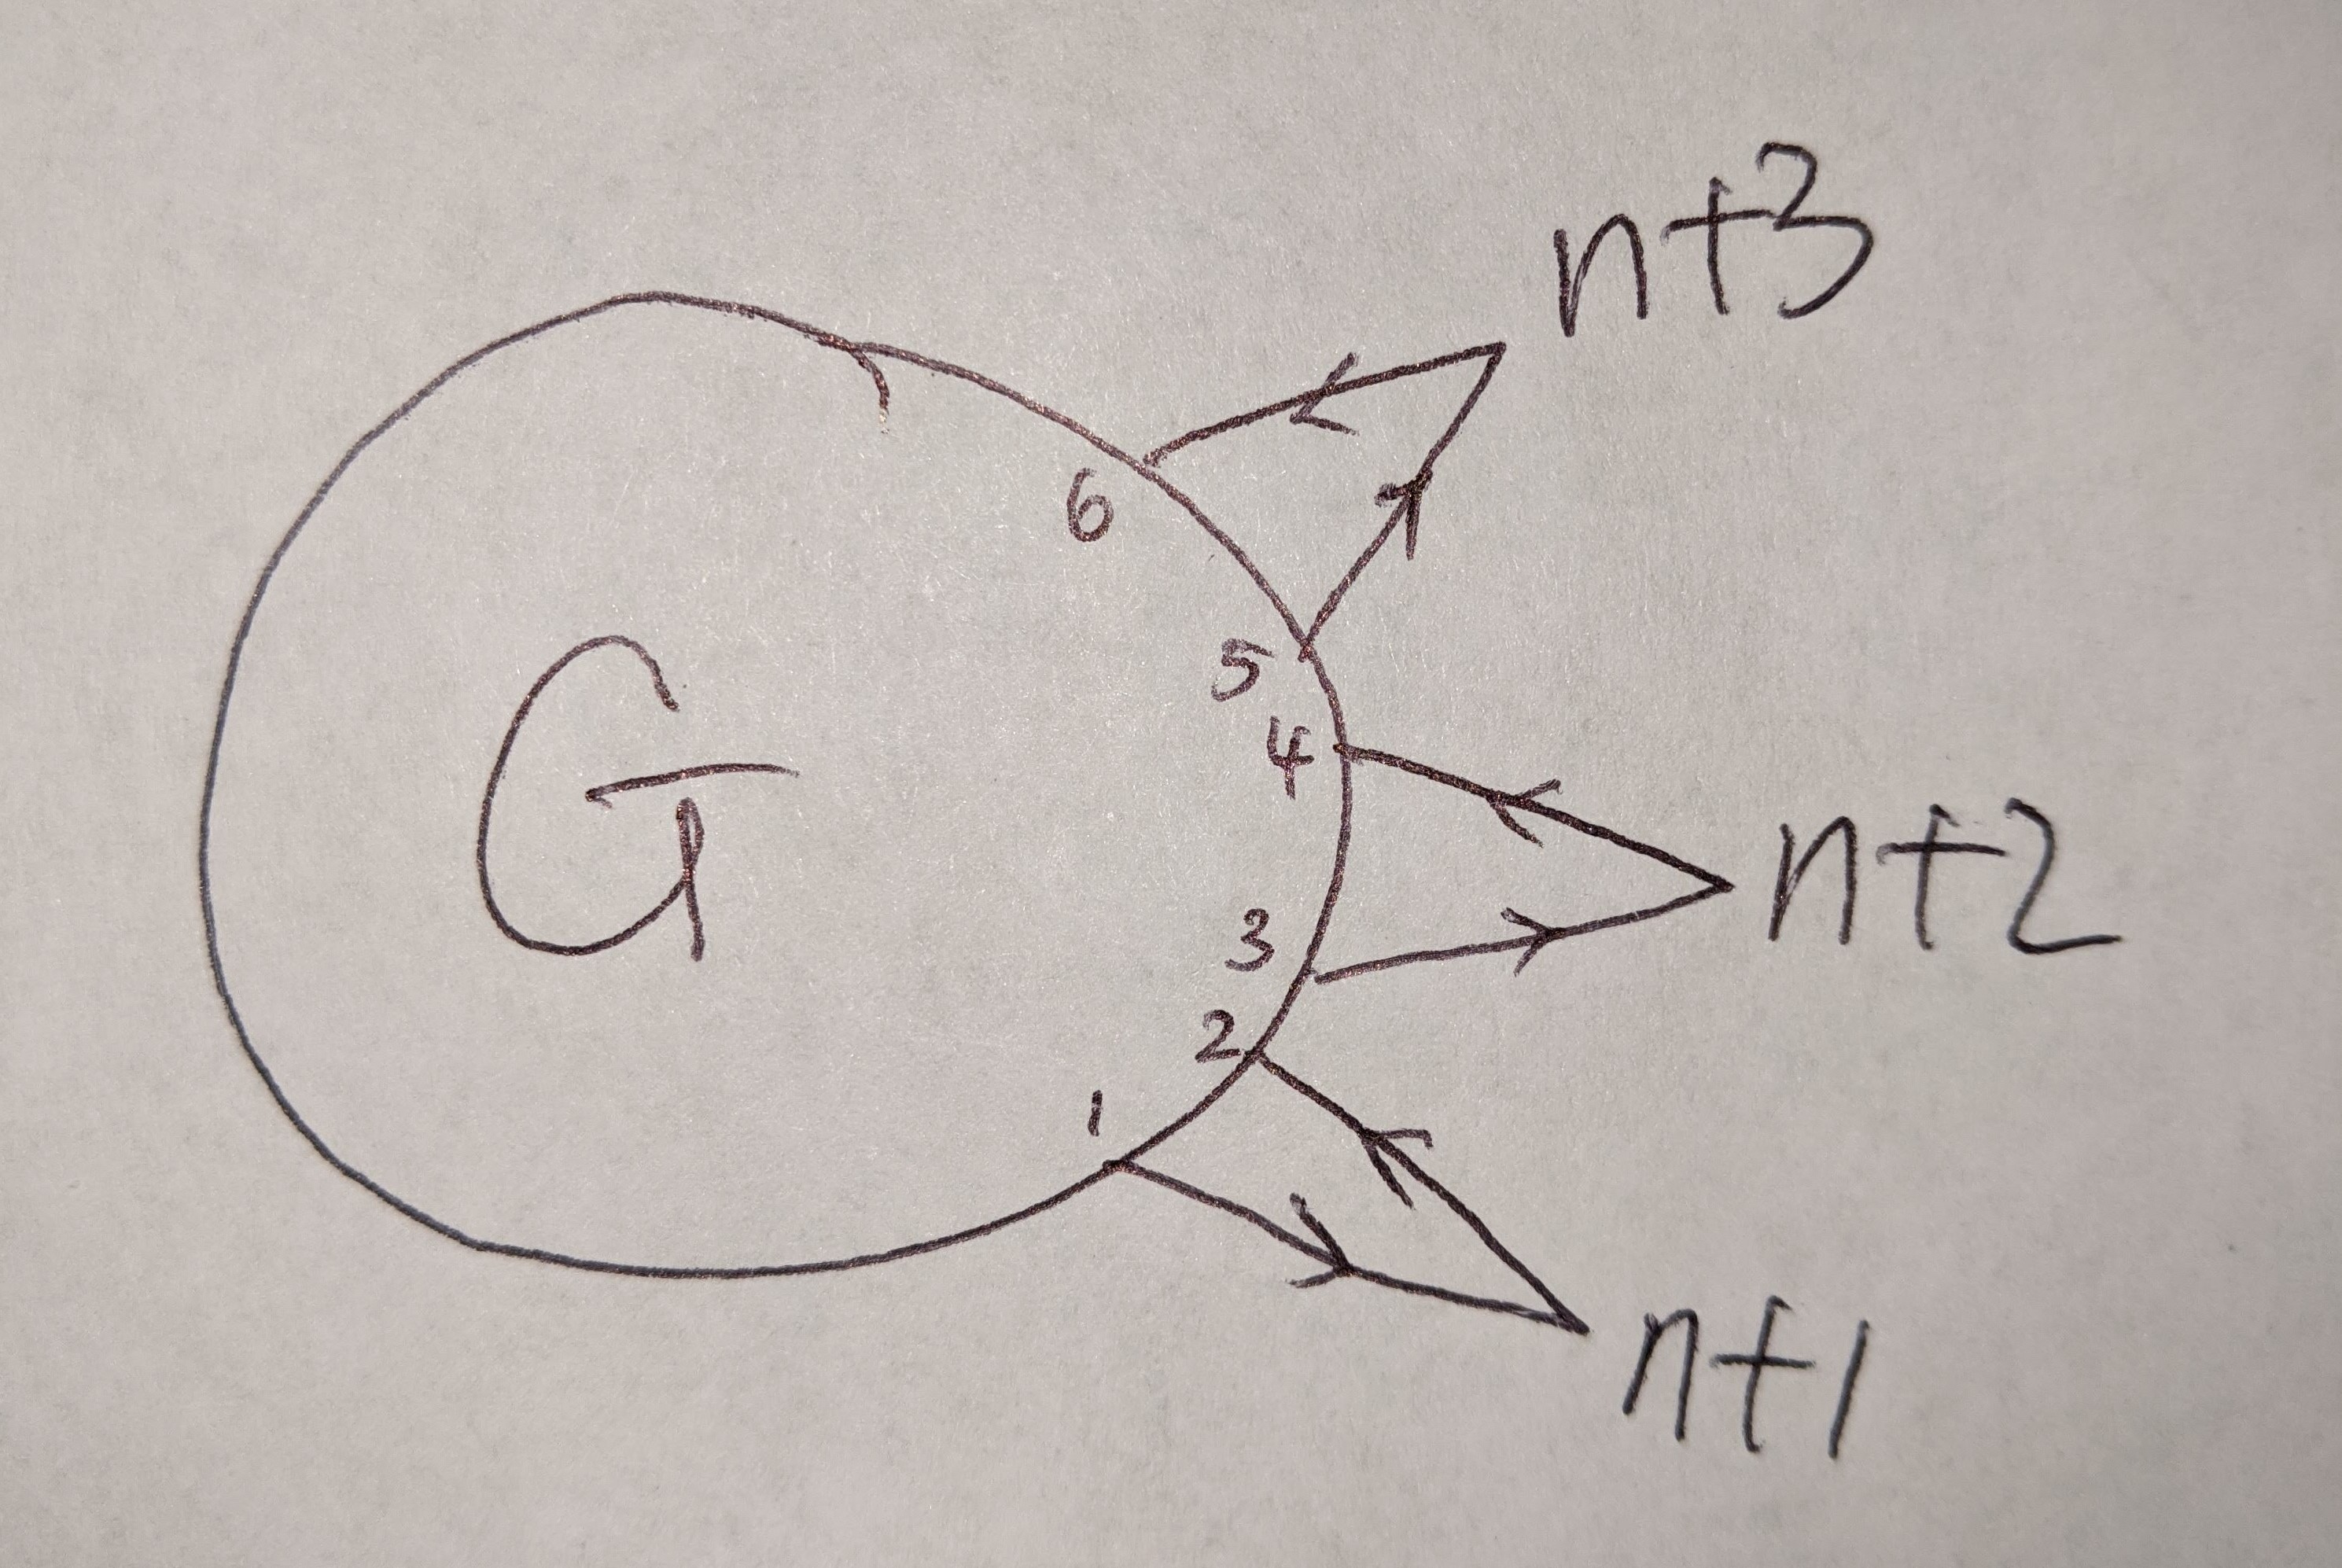
\includegraphics[scale=0.025]{graph3_1.jpg}
\ethm

\bpf
Let $VH(G)$ be directed handle graph with 3 handles, and let $T$ be a spanning tree in $VH(G)$. Suppose $T$ is rooted at vertex $v_5\in V(G)$. Let $e_1$ be the inflow edge to node 2, $e_2$ be the inflow edge to node 4, and $e_3$ be the inflow edge to node 6. Then there are four cases.

Case 1. $e_1\notin VH(G)$, $e_2\notin VH(G)$, and $e_3\notin VH(G)$. Then the number of spanning tree is $\tau(G)$.

Case 2. Only one of $e_1, e_2, e_3$ is in $VH(G)$. 

By \Cref{symhandle}, there does not exist a path between $v_1$ and $v_2$, or between $v_3$ and $v_4$, or between $v_5$ and $v_6$ .

So, the subgraph rooted at node 1 is $\tau_{(1)(2)}(G)+ \tau_{(3)(4)}(G)+ \tau_{(5)(6)}(G)$

Case 3. Two of $e_1, e_2, e_3$ are in $VH(G)$. 
\begin{enumerate}
    \item $e_1\in VH(G)$, $e_2\in VH(G)$, and $e_3\notin VH(G)$.
    
    By \cref{symhandle}, there does not exist path between node 1,2 and node 3,4. Then the number of spanning tree is $\tau_{(135)(2)(4)}(G) + \tau_{(15)(23)(4)}(G) + \tau_{(35)(14)(2)}(G)$.
    
    \item $e_1\in VH(G)$, $e_2\notin VH(G)$, and $e_3\in VH(G)$.
    
    By \cref{symhandle}, there does not exist path between node 1,2 and node 5,6. Then the number of spanning tree is $\tau_{(15)(2)(6)}(G) + \tau_{(5)(16)(2)}(G)$.
    
    \item $e_1\notin VH(G)$, $e_2\in VH(G)$, and $e_3\in VH(G)$.
    
    By \cref{symhandle}, there does not exist path between node 3,4 and node 5,6. Then the number of spanning tree is $\tau_{(53)(4)(6)}(G) + \tau_{(5)(36)(4)}(G)$.
\end{enumerate}

Case 4. All of $e_1, e_2, e_3$ are in $VH(G)$. 

By \cref{symhandle}, there does not exist path between node 1,2 and node 3,4 and node 5,6. Then the number of spanning tree is $$\tau_{(135)(2)(4)(6)}(G) + \tau_{(15)(23)(4)(6)}(G) + \tau_{(15)(36)(2)(4)}(G) + \tau_{(35)(14)(2)(6)}(G) + \tau_{(35)(16)(2)(4)}(G)$$

Therefore, the total number of subgraphs of $VH(G)$ is  
\begin{equation*}
    \begin{split}
        \tau(VH_3(G))_5 &= \tau(G) + \tau_{(1)(2)}(G)+ \tau_{(3)(4)}(G) + \tau_{(5)(6)}(G)\\ 
        &+ \tau_{(53)(4)(6)}(G) + \tau_{(5)(36)(4)}(G) + \tau_{(15)(2)(6)}(G) + \tau_{(5)(16)(2)}(G)\\
        &+ \tau_{(135)(2)(4)}(G) + \tau_{(15)(23)(4)}(G) + \tau_{(35)(14)(2)}(G)\\
        &+ \tau_{(135)(2)(4)(6)}(G) + \tau_{(15)(23)(4)(6)}(G) + \tau_{(15)(36)(2)(4)}(G)\\
&+ \tau_{(35)(14)(2)(6)}(G) + \tau_{(35)(16)(2)(4)}(G)
    \end{split}
\end{equation*}
\epf

\bthm
{\bf (Rooted at 6)}
Let $VH(G)$ be directed handle graph with 3 handles, and let $T$ be a spanning tree in $VH(G)$. If $T$ is rooted at vertex $v_6\in V(G)$ as shown in the picture below,
then the total number of subgraphs of $VH(G)$ is  
\[
\tau(VH_3(G))_6 = \tau(G) + \tau_{(1)(2)}(G)+ \tau_{(3)(4)}(G) + \tau_{(1)(23)(4)}(G)+ \tau_{(13)(2)(4)}(G)
\]
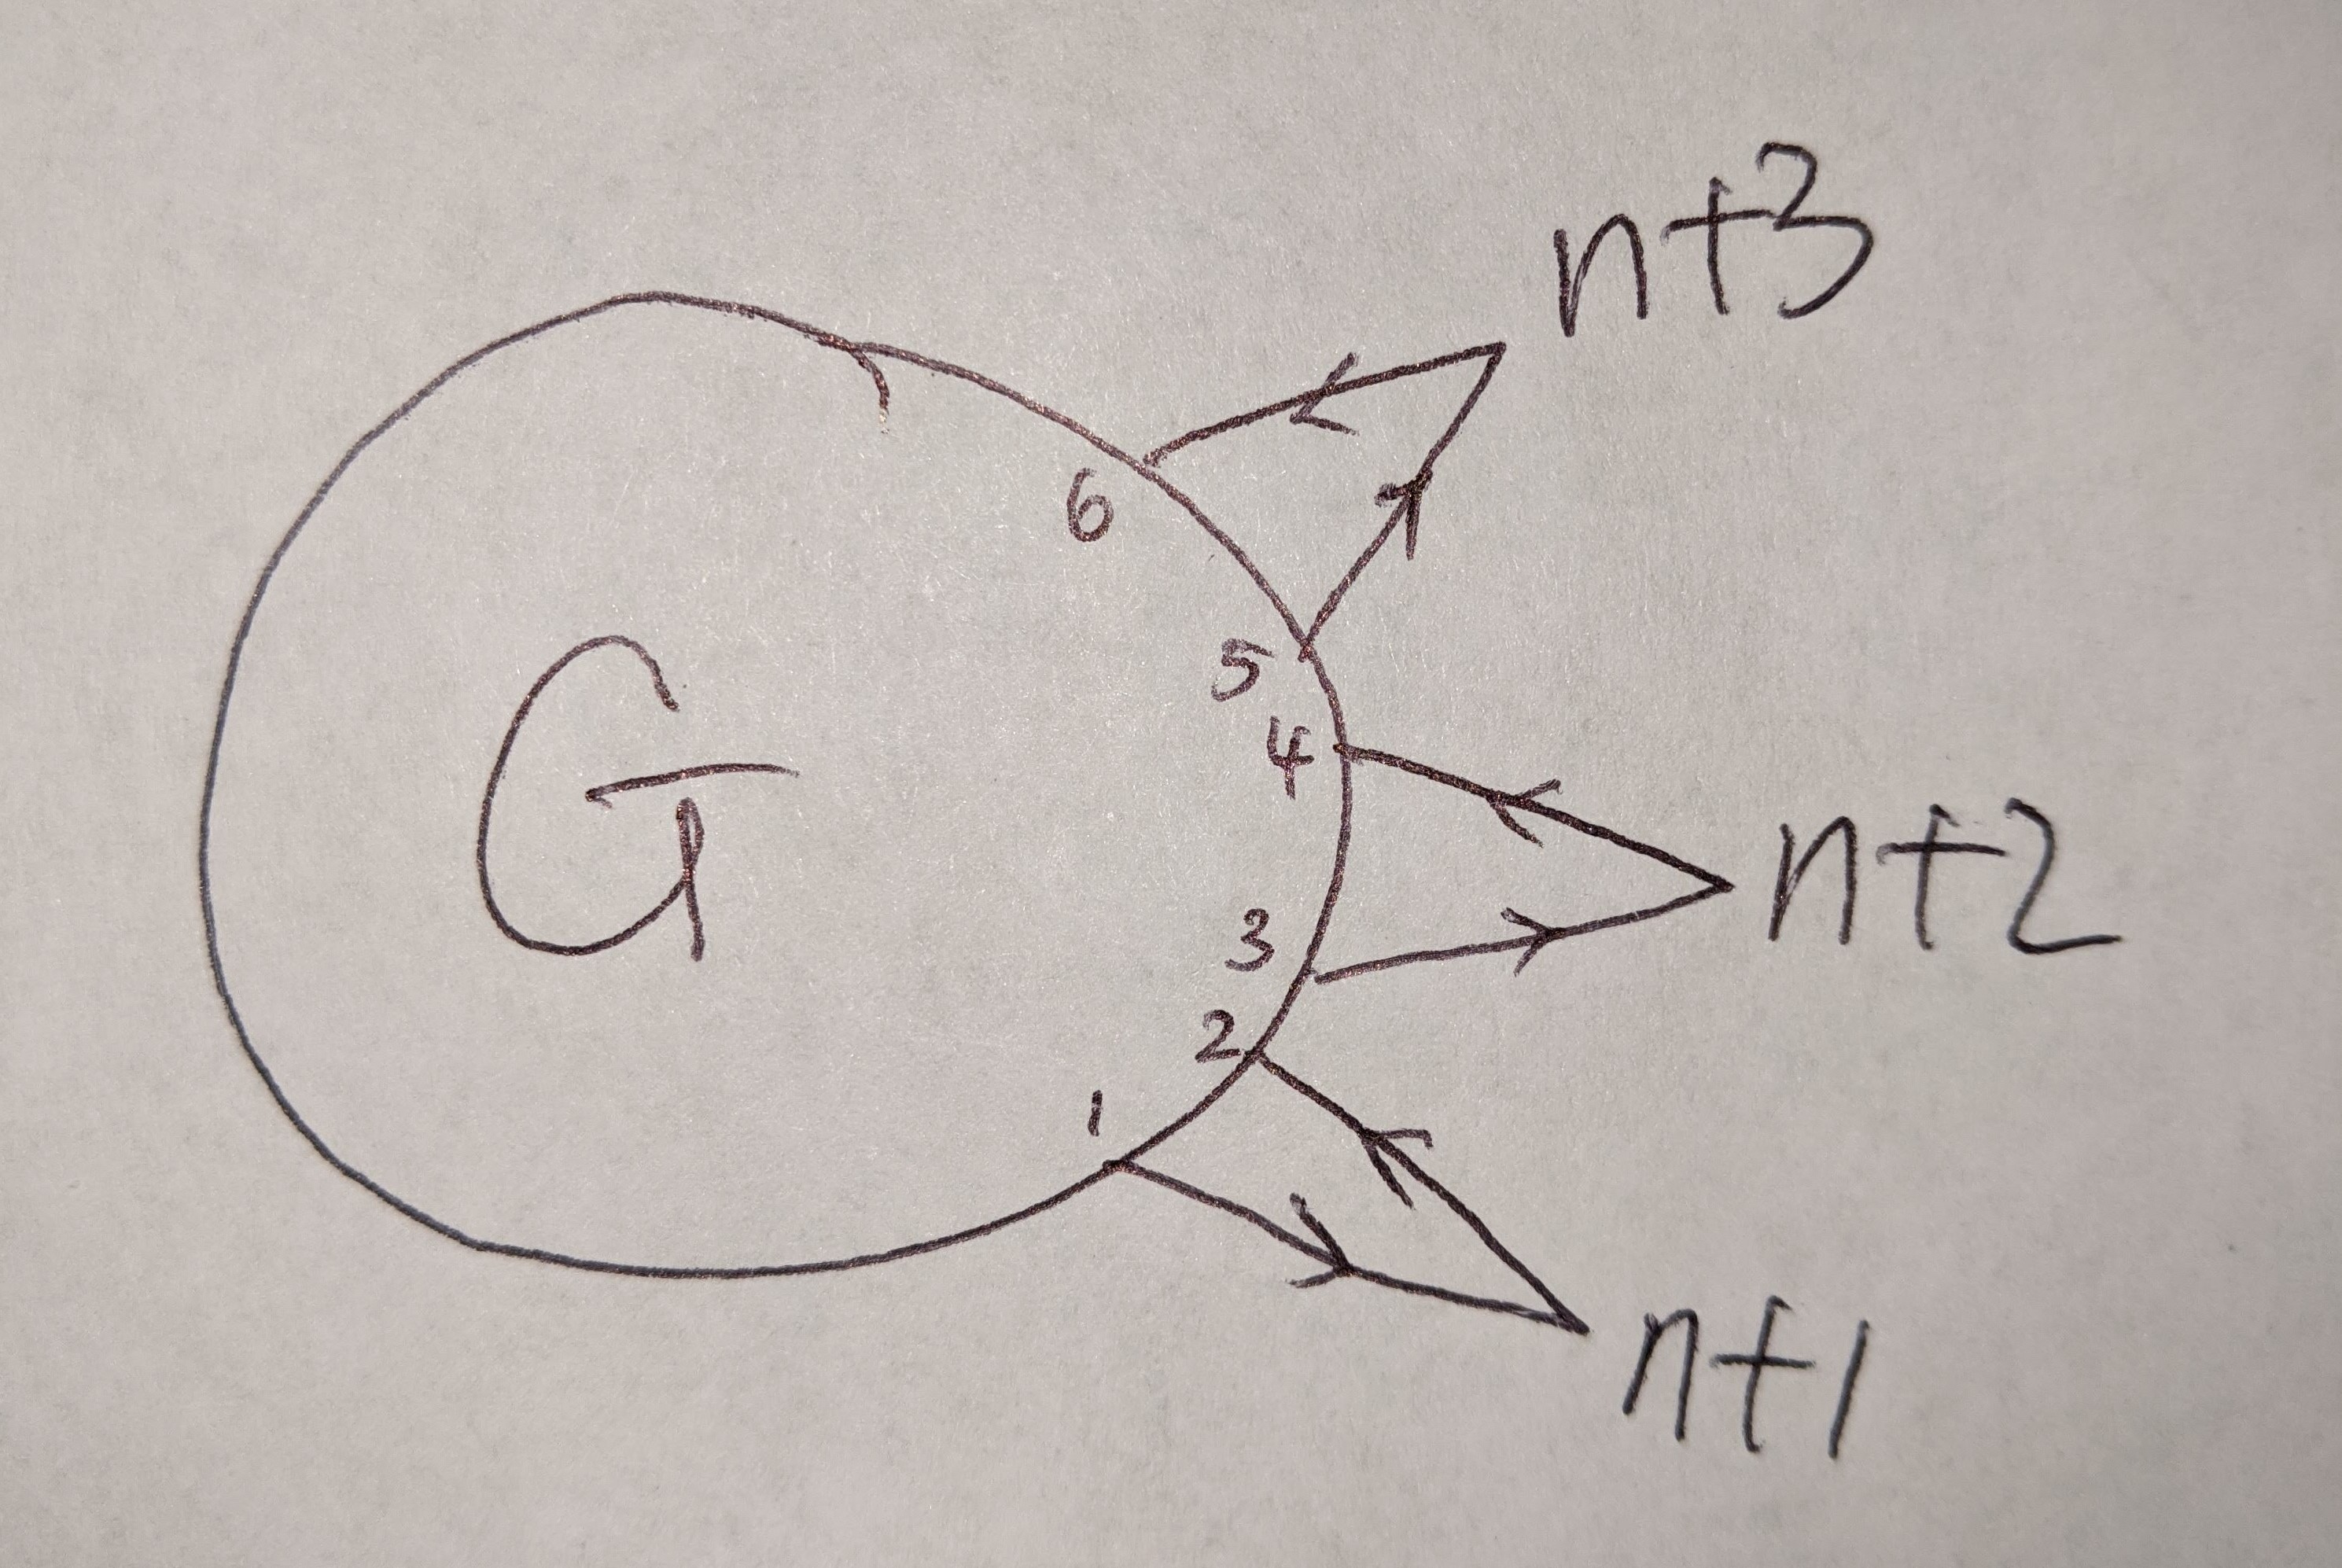
\includegraphics[scale=0.025]{graph3_1.jpg}
\ethm

\bpf
Let $VH(G)$ be directed handle graph with 3 handles, and let $T$ be a spanning tree in $VH(G)$. Suppose $T$ is rooted at vertex $v_6\in V(G)$. Let $e_1$ be the inflow edge to node 2, $e_2$ be the inflow edge to node 4, and $e_3$ be the inflow edge to node 6. Since $T$ is rooted at 6, $e_3 \notin VH(G)$. Therefore, there are three cases.

Case 1. Case 1. $e_1\notin VH(G)$, and $e_3\notin VH(G)$. Then the number of spanning tree is $\tau(G)$.

Case 2. Only one of $e_1, e_2$ is in $VH(G)$. 

By \Cref{symhandle}, there does not exist a path between $v_1$ and $v_2$ or between $v_3$ and $v_4$.

So, the subgraph rooted at node 2 is $\tau_{(1)(2)}(G)+ \tau_{(3)(4)}(G)$

Case 3. Both of $e_2, e_3$ are in $VH(G)$.

By \cref{symhandle}, there does not exist path between node 3,4 and 5,6. Then the number of spanning tree is $\tau_{(1)(23)(4)}(G)+ \tau_{(13)(2)(4)}(G)$.

Therefore, the total number of subgraphs of $VH(G)$ is  \[
\tau(VH_3(G))_6 = \tau(G) + \tau_{(1)(2)}(G)+ \tau_{(3)(4)}(G) + \tau_{(1)(23)(4)}(G)+ \tau_{(13)(2)(4)}(G)
\]
\epf

\bthm
{\bf (Rooted at 0)}
Let $VH(G)$ be directed handle graph with 3 handles, and let $T$ be a spanning tree such that $T\in VH(G)$. If $T$ is rooted at vertex $v_0\in V(G)$ as shown in the picture below,
then the total number of subgraphs of $VH(G)$ is  
\begin{equation*}
    \begin{split}
        \tau(VH_3(G))_0 &= \tau(G) + \tau_{(1)(2)}(G)+ \tau_{(3)(4)}(G) + \tau_{(5)(6)}(G)\\ 
        &+ \tau_{(01)(23)(4)}(G) + \tau_{(03)(14)(2)}(G) + \tau_{(013)(2)(4)}(G)\\
        &+ \tau_{(03)(24)(6)}(G) + \tau_{(05)(4)(36)}(G) + \tau_{(035)(4)(6)}(G)\\
        &+ \tau_{(01)(25)(6)}(G) + \tau_{(05)(2)(16)}(G) + \tau_{(015)(2)(6)}(G)\\
        &+ \tau_{(0135)(2)(4)(6)}(G) + \tau_{(013)(25)(4)(6)}(G) + \tau_{(013)(45)(2)(6)}(G)\\
        &+ \tau_{(015)(23)(4)(6)}(G) + \tau_{(015)(36)(2)(4)}(G) + \tau_{(035)(41)(2)(6)}(G) + \tau_{(035)(61)(2)(4)}(G)\\
        &+ \tau_{(01)(23)(45)(6)}(G) + \tau_{(01)(25)(36)(4)}(G) + \tau_{(01)(235)(4)(6)}(G)\\
        &+ \tau_{(03)(45)(16)(2)}(G) + \tau_{(03)(14)(25)(6)}(G) + \tau_{(03)(145)(2)(6)}(G)\\
        &+ \tau_{(05)(16)(23)(4)}(G) + \tau_{(05)(36)(14)(2)}(G) + \tau_{(05)(163)(2)(4)}(G)
    \end{split}
\end{equation*}
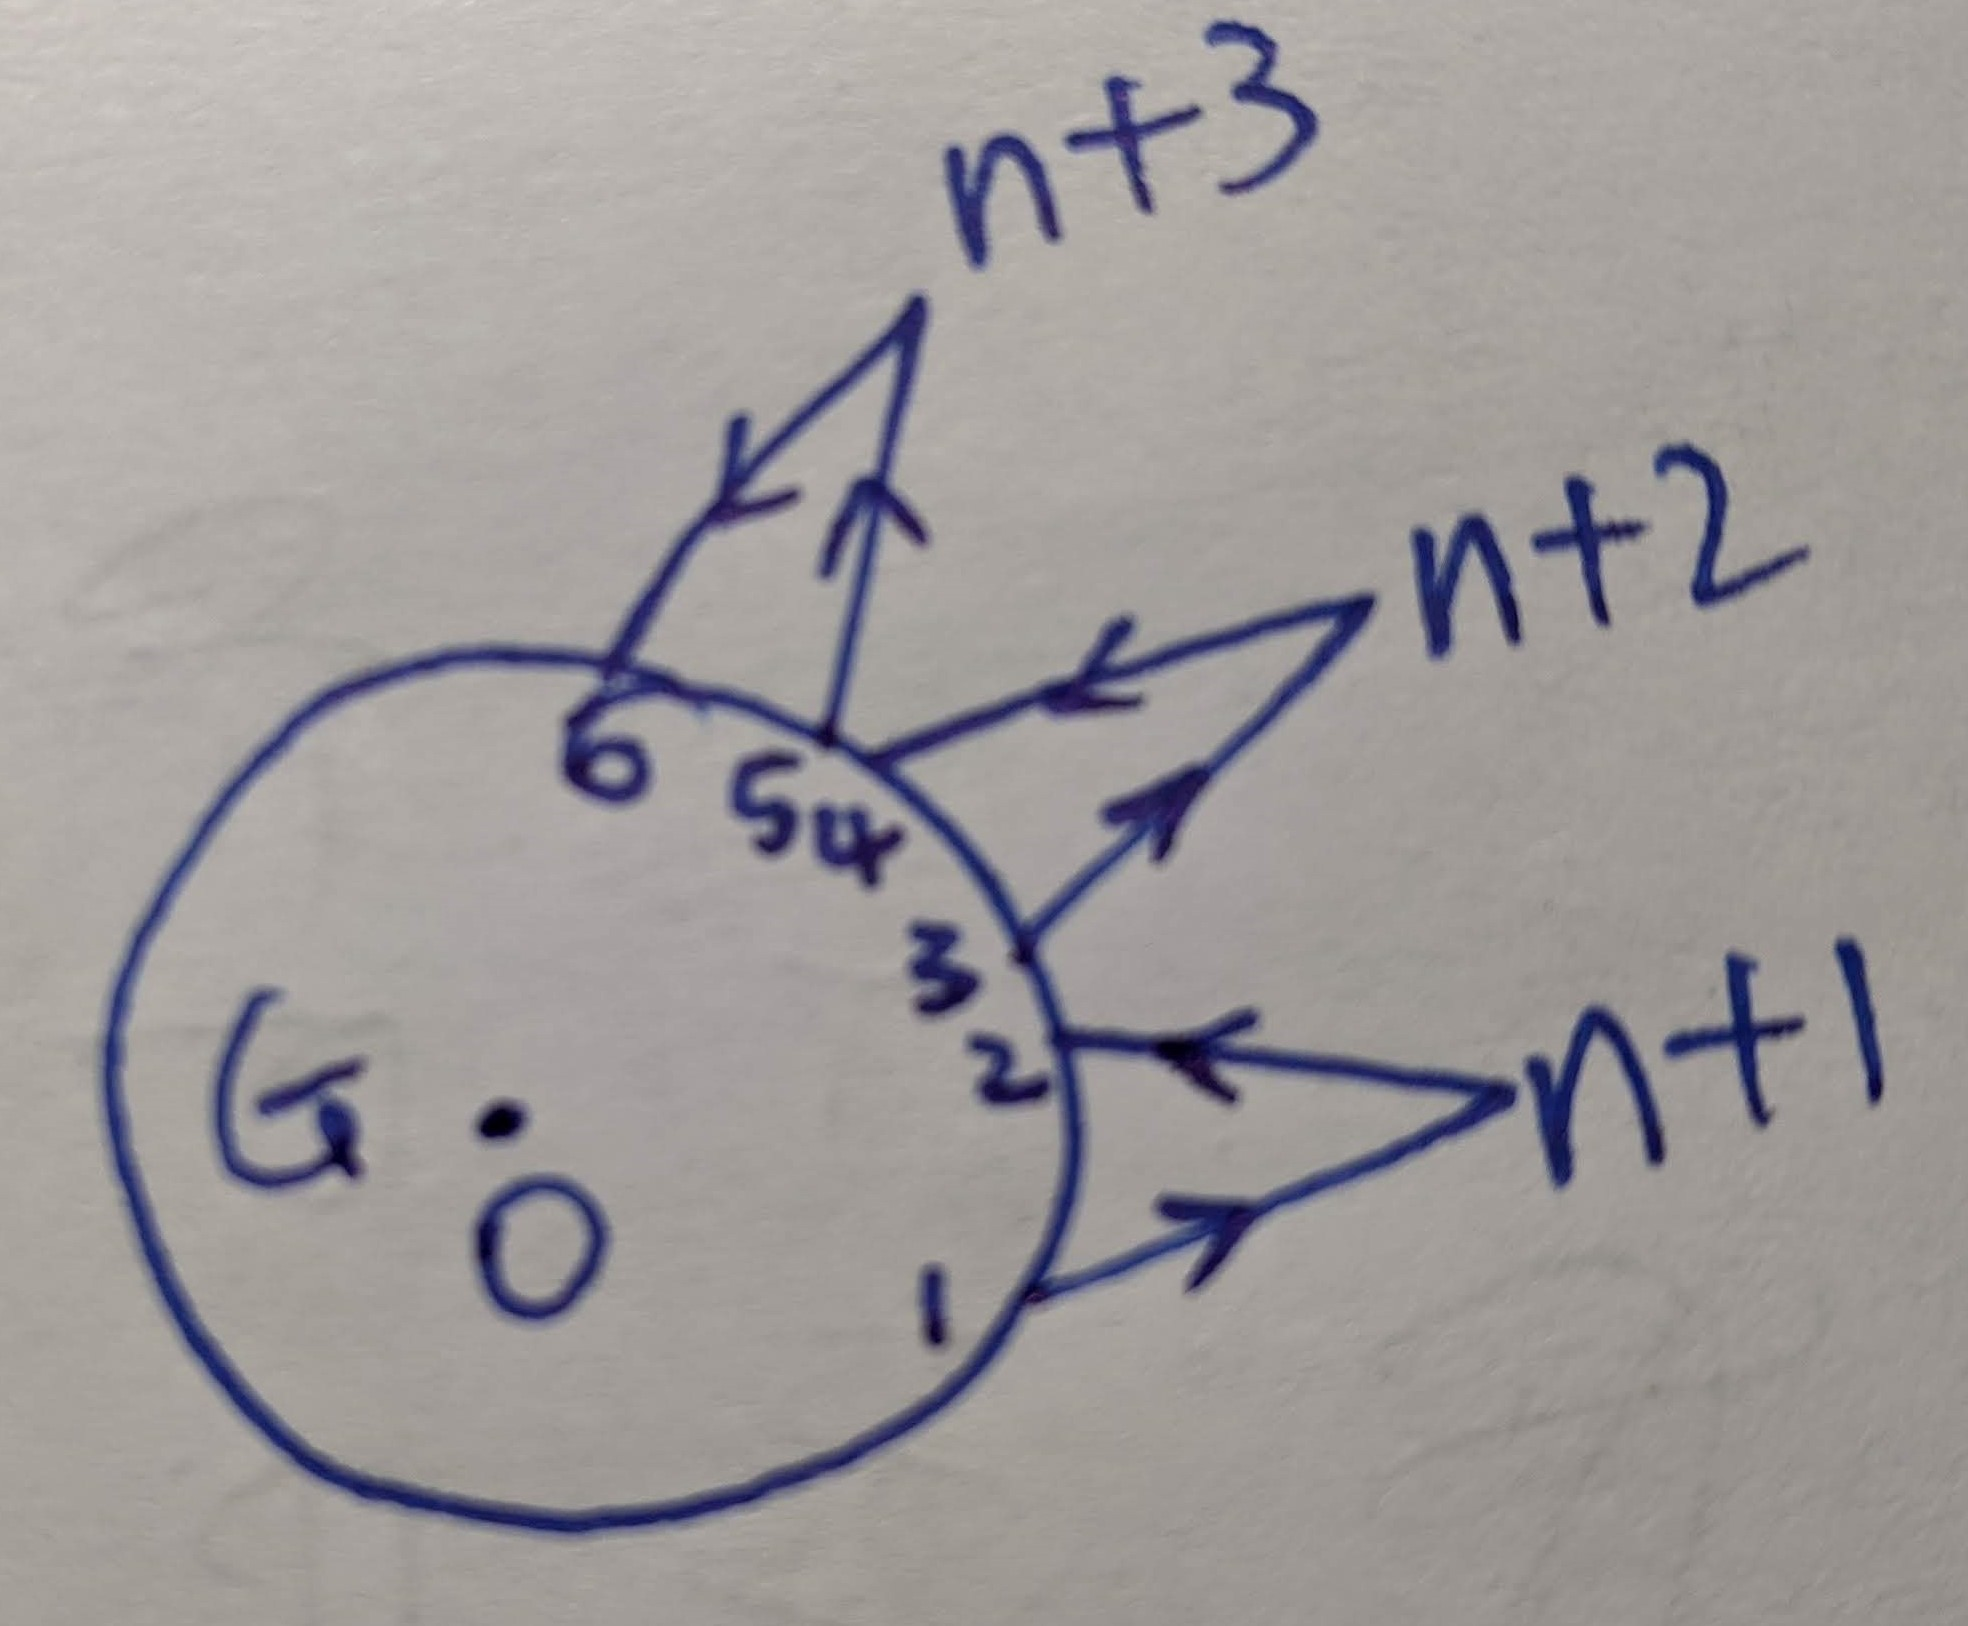
\includegraphics[scale=0.025]{graph3_0.jpg}
\ethm

\bpf
Let $VH(G)$ be directed handle graph with 3 handles, and let $T$ be a spanning tree such that $T\in VH(G)$. Suppose $T$ is rooted at vertex $v_0\in V(G)$. Let $e_1$ be the inflow edge to node 2, $e_2$ be the inflow edge to node 4, and $e_3$ be the inflow edge to node 6. Then there are four cases.

Case 1. $e_1\notin VH(G)$, $e_2\notin VH(G)$, and $e_3\notin VH(G)$. Then the number of spanning tree is $\tau(G)$.

Case 2. Only one of $e_1, e_2, e_3$ is in $VH(G)$. 

By \Cref{symhandle}, there does not exist a path between $v_1$ and $v_2$, or between $v_3$ and $v_4$, or between $v_5$ and $v_6$ .

So, the subgraph rooted at node 1 is $\tau_{(1)(2)}(G)+ \tau_{(3)(4)}(G)+ \tau_{(5)(6)}(G)$

Case 3. Two of $e_1, e_2, e_3$ are in $VH(G)$. 
\begin{enumerate}
    \item $e_1\notin VH(G)$, $e_2\in VH(G)$, and $e_3\in VH(G)$.
    
    By \cref{symhandle}, there does not exist path between node 3,4 and node 5,6. Then the number of spanning tree is \\$\tau_{(03)(24)(6)}(G) + \tau_{(05)(4)(36)}(G) + \tau_{(035)(4)(6)}(G)$.
    
    \item $e_1\in VH(G)$, $e_2\notin VH(G)$, and $e_3\in VH(G)$.
    
    By \cref{symhandle}, there does not exist path between node 1,2 and node 5,6. Then the number of spanning tree is \\$\tau_{(01)(25)(6)}(G) + \tau_{(05)(2)(16)}(G) + \tau_{(015)(2)(6)}(G)$.
    
    \item $e_1\in VH(G)$, $e_2\in VH(G)$, and $e_3\notin VH(G)$.
    By \cref{symhandle}, there does not exist path between node 1,2 and node 3,4. Then the number of spanning tree is $\tau_{(01)(23)(4)}(G) + \tau_{(03)(14)(2)}(G) + \tau_{(013)(2)(4)}(G)$.
\end{enumerate}

Case 4. All of $e_1, e_2, e_3$ are in $VH(G)$. 

By \cref{symhandle}, there does not exist path between node 1,2 and node 3,4 and node 5,6. Then the number of spanning tree is $\tau_{(0135)(2)(4)(6)}(G) + \tau_{(013)(25)(4)(6)}(G) + \tau_{(013)(45)(2)(6)}(G) + \tau_{(015)(23)(4)(6)}(G) + \tau_{(015)(36)(2)(4)}(G) + \tau_{(035)(41)(2)(6)}(G) + \tau_{(035)(61)(2)(4)}(G) + \tau_{(01)(23)(45)(6)}(G) + \tau_{(01)(25)(36)(4)}(G) + \tau_{(01)(235)(4)(6)}(G) + \tau_{(03)(45)(16)(2)}(G) + \tau_{(03)(14)(25)(6)}(G) + \tau_{(03)(145)(2)(6)}(G) + \tau_{(05)(16)(23)(4)}(G) + \tau_{(05)(36)(14)(2)}(G) + \tau_{(05)(163)(2)(4)}(G)$.
\\

Therefore, the total number of subgraphs of $VH(G)$ is  
\begin{equation*}
    \begin{split}
        \tau(VH_3(G))_0 &= \tau(G) + \tau_{(1)(2)}(G)+ \tau_{(3)(4)}(G) + \tau_{(5)(6)}(G)\\ 
        &+ \tau_{(01)(23)(4)}(G) + \tau_{(03)(14)(2)}(G) + \tau_{(013)(2)(4)}(G)\\
        &+ \tau_{(03)(24)(6)}(G) + \tau_{(05)(4)(36)}(G) + \tau_{(035)(4)(6)}(G)\\
        &+ \tau_{(01)(25)(6)}(G) + \tau_{(05)(2)(16)}(G) + \tau_{(015)(2)(6)}(G)\\
        &+ \tau_{(0135)(2)(4)(6)}(G) + \tau_{(013)(25)(4)(6)}(G) + \tau_{(013)(45)(2)(6)}(G)\\
        &+ \tau_{(015)(23)(4)(6)}(G) + \tau_{(015)(36)(2)(4)}(G) + \tau_{(035)(41)(2)(6)}(G) + \tau_{(035)(61)(2)(4)}(G)\\
        &+ \tau_{(01)(23)(45)(6)}(G) + \tau_{(01)(25)(36)(4)}(G) + \tau_{(01)(235)(4)(6)}(G)\\
        &+ \tau_{(03)(45)(16)(2)}(G) + \tau_{(03)(14)(25)(6)}(G) + \tau_{(03)(145)(2)(6)}(G)\\
        &+ \tau_{(05)(16)(23)(4)}(G) + \tau_{(05)(36)(14)(2)}(G) + \tau_{(05)(163)(2)(4)}(G)
    \end{split}
\end{equation*}
\epf

\end{document}
